\documentclass{article}
\usepackage[fleqn]{amsmath}
\usepackage{amssymb,graphicx,color,graphicx,slashed, microtype, parskip, enumitem, extarrows, needspace}
%\usepackage[utf8x]{inputenc}
\usepackage[top=1.5cm, bottom=1.5cm, right=6cm, left=1.5cm, heightrounded, marginparwidth=5cm, marginparsep=0.5cm]{geometry}

\hbadness = 10000
\hfuzz=100pt 
    
\usepackage{marginnote}
\renewcommand*{\marginfont}{\footnotesize}

\usepackage{hyperref}
\hypersetup{colorlinks=true, urlcolor=NavyBlue, bookmarksdepth=3}

\makeatletter\newcommand{\@minipagerestore}{\setlength{\parskip}{\medskipamount}}\makeatother

% =============== Index ===========================

\usepackage[nonewpage]{imakeidx}
\makeindex

% =============== Color Definitions ===============
    
\usepackage[svgnames]{xcolor}
\colorlet{ColorTitle}{Black}
\colorlet{ColorSectionName}{Black}
\colorlet{ColorBoxFG}{Gray}
\colorlet{ColorBoxText}{Black}
\colorlet{ColorBoxBG}{White}


% =============== Title Style ===============
    
\usepackage{titling} % Allows custom title configuration
    
\newcommand{\HorRule}{\color{ColorTitle}\rule{\linewidth}{1pt}} % Defines the gold horizontal rule around the title
    
\pretitle{
    \vspace{-50pt} % Move the entire title section up
    \HorRule\vspace{9pt} % Horizontal rule before the title
    \fontsize{27}{36}\usefont{OT1}{phv}{b}{n}\selectfont
    \color{ColorTitle} % Text colour for the title and author(s)
}
    
\posttitle{\par\vskip 15pt} % Whitespace under the title
    
\preauthor{\fontsize{17}{0}\usefont{OT1}{phv}{m}{n}\selectfont\color{ColorTitle}} % Anything that will appear before \author is printed
    
\postauthor{\par\HorRule}

\newcommand{\COURSENAME}{\href{http://phyw.people.ust.hk/teaching/PHYS2022-2015/}{\textcolor{black}{PHYS 2022}}}
\newcommand{\YW}{\href{http://phyw.people.ust.hk/}{\textcolor{black}{Yi Wang}}}
\newcommand{\PHYS}{\href{http://physics.ust.hk}{\textcolor{black}{Department of Physics}}}
\newcommand{\HKUST}{\href{http://www.ust.hk/}{\textcolor{black}{HKUST}}}
\author{\COURSENAME, \YW, \PHYS, \HKUST}

\date{}

% =============== Section Name Style ===============
    
\usepackage{titlesec}
    
\titleformat{\section}
    {\fontsize{15}{20}\usefont{OT1}{phv}{b}{n}\color{ColorSectionName}}
    {\thesection}{1em}{}
    %[{\vspace{0.2cm}\titlerule[0.8pt]}]
    
\titleformat{\subsection}
    {\fontsize{14}{20}\usefont{OT1}{phv}{m}{n}\color{ColorSectionName}}
    {\thesubsection}{1em}{}
    
\titleformat{\subsubsection}
    {\fontsize{12}{20}\usefont{OT1}{phv}{m}{n}\color{ColorSectionName}}
    {}{0em}{}
      
\setcounter{secnumdepth}{4}
        
% =============== Box Style ===============
    
\usepackage[most]{tcolorbox}
    
\newtcolorbox{tbox}[1]{
    colback=ColorBoxBG, colframe=ColorBoxFG, coltext=ColorBoxText,
    sharp corners, enhanced, breakable, parbox=false,
    before skip=1em, after skip=1em,
    title={#1}, fonttitle=\usefont{OT1}{phv}{b}{n}, 
    attach boxed title to top left={yshift=-0.1mm}, boxed title style={sharp corners, colback=ColorBoxFG, left=0.405cm},
    rightrule=-1pt,toprule=-1pt, bottomrule=-1pt
}

\newtcolorbox{mtbox}[1]{
    colback=ColorBoxBG, colframe=ColorBoxFG, coltext=ColorBoxText,
    sharp corners, enhanced, breakable, parbox=false,
    before skip=1em, after skip=1em,
    title={#1}, fonttitle=\usefont{OT1}{phv}{b}{n},
    attach boxed title to top left={yshift=-0.1mm}, boxed title style={sharp corners, colback=ColorBoxFG, left=0.15cm},
    rightrule=-1pt,toprule=-1pt, bottomrule=-1pt, 
    left=0.5em
}

% =============== tikz has to be loaded after xcolor
\usepackage{tikz}

\newcommand*\enumlabel[1]{\tikz[baseline=(char.base)]{
			\node[shape=rectangle,inner sep=2pt,fill=ColorBoxFG] (char) 
			{\fontsize{7}{20}\usefont{OT1}{phv}{b}{n}{\textcolor{ColorBoxBG}{#1}}};}}

% =============== Useful shortcuts ===============

\newcommand\wref[1]{{\hypersetup{linkcolor=white}\ref{#1}}}  

\newcommand{\textbox}[2]{
    \begin{tbox}{#1}
        #2
    \end{tbox}
}

\newcommand{\mtextbox}[2]{\marginnote{
    \begin{mtbox}{#1}
        #2
    \end{mtbox}}
}

\newcommand{\mnewline}{\vspace{0.5em}\newline}

\newcommand{\titem}[1]{
    \begin{itemize}[label=\color{ColorBoxFG}$\blacktriangleright$, leftmargin=0mm, labelsep=0.27cm, topsep=0.5em
        %, itemsep=1ex
        ]
        #1
    \end{itemize}
}

\newcommand{\mtitem}[1]{
    \begin{itemize}[label={\color{ColorBoxFG}$\blacktriangleright$}, leftmargin=0mm, labelsep=1mm, topsep=0.5em
        %, itemsep=1ex
        ]
        #1
    \end{itemize}
}

\newcommand{\itembox}[3]{
    \begin{tbox}{#1}
        #2
        \titem{#3}
    \end{tbox}
}

\newcommand{\mitembox}[3]{
    \marginnote{
    \begin{mtbox}{#1}
        #2
        \mtitem{#3}
	\end{mtbox}
    }
}

\newcommand{\tenum}[1]{
    \begin{enumerate}[label=\protect\enumlabel{\arabic*}, leftmargin=0mm, labelsep=0.265cm, topsep=0.5em
        %, itemsep=1ex
        ]
        #1
    \end{enumerate}
}

\newcommand{\enumbox}[3]{
    \begin{tbox}{#1}
        #2
        \tenum{#3}
    \end{tbox}
}

\newcommand{\twocol}[5]{
    \begin{minipage}[t][][b]
        {#1\textwidth}
        #4        
    \end{minipage}
    \hspace{#2\textwidth}
    \begin{minipage}[t][][b]
        {#3\textwidth}
        #5
    \end{minipage}
}

\newcommand{\cg}[2]{
    \begin{center}
        \includegraphics[width=#1\textwidth]{#2}
    \end{center}
}

\newcommand{\tbar}{
    ~\newline
    {\color{ColorBoxFG}
    \hbox to 0.15\textwidth{\leaders\hbox to 5pt{\hss  \hss}\hfil} 
    \hbox to 0.7\textwidth{\leaders\hbox to 5pt{\hss . \hss}\hfil}}
    \mnewline
}

% =============== Filter unwanted warnings
\usepackage{silence}
\WarningsOff[tcolorbox]
\hbadness=1000000


\usepackage{wasysym}
\graphicspath{{1_fig/}}
\title{第一章\ 狭义相对论}

\usepackage{ctex}


\begin{document}

\maketitle

让我们从一个思想实验开始我们探索物理的奇妙旅程——王二乘坐宇宙飞船前往距离我们5光年远的一颗恒星,他到达后将立即返回地球。王三送他走并等他回来。假设宇宙飞船的运行速度几乎与光速 $c$ 一样快,例如 $v=0.995c$
\cg{0.7}{spaceship5}

令人惊讶的是,在 $v\sim c$ 处,事物的行为与我们的日常经验(也就是牛顿力学)截然不同。让我们看看他们发现的一些神奇的事实:

\mitembox{对于时空的理解}{
	随着我们对自然更好的了解,我们对时空也有了更深入的理解。到目前为止,科学家们依然在努力的探索。
	}{
	\item 牛顿力学: 空间和时间对于物质来说是绝对独立的。
	\item 狭义相对论:空间和时间是统一的,并且取决于观察者的运动(就像物体的相对方向会随着观察者的转动而改变)。
	\item 广义相对论: 空间和时间可以被物体弯曲。
	\item 量子引力(推测):空间和时间可能是从全息和量子纠缠中演生出来的。我们还没有完全理解它,但是我们从中得到的这些线索是深刻的。

}

\itembox{王三对王二旅行的观察}{}{
	\item 王三给王二写了一封信,王二大约在同一时间也给王三写了一封信。王三认为他的信写的更早,同时王二也坚持认为他自己的信写得更早。他们考虑到了光需要时间才能传播,但即使如此,他们也无法解决这个纷争。

	\item 王三发现当 $v\sim c$ 时,飞船变得更重了,王二需要越来越多的能量来使飞船加速。
	\item 当王二回来时,王三已经过去了 10 年。但对于王二来说,他的时钟,他的感觉,关于他的一切都表明,仅仅过去了一年。
} 

这里发生了什么?学完这部分内容,你就会发现,还有更多神奇的事情。事实上,我们必须以一种与我们天真的想法截然不同的方式来思考空间和时间。

\section{相对性原理}\label{sec:principles-relativity}

\subsection{伽利略变换}

想象一下:
\marginnote{“向外看”指的是通过任何方式与汽车外部的连接,比如使用光、声、引力波等。我们忽略地球的自转,从而我们可以认为王二和王三处于惯性坐标系(也就是他们的运动是匀速的)。
}
在图~\ref{fig:grel}中,王二在一辆封闭的汽车中以恒定速度 $\mathbf{v}$ 相对于地面移动。如果王二不看车外,他怎么会发现他在地面上移动呢?


答案是如果王二不看车外,无论他尝试什么活动/实验,他都发现与汽车没有移动时没有区别。用物理学的语言来说,他这时探索到的自然界的定律与他不动时探索到的定律是完全相同的。

在1632年,伽利略说这对所有物理定律和所有惯性系都是正确的。这被称为伽利略相对性原理。令人惊叹的是,据我们所知,这一拥有近 400 年历史的原理在现在仍然适用。
 
\begin{figure}[htbp] 
	\centering
	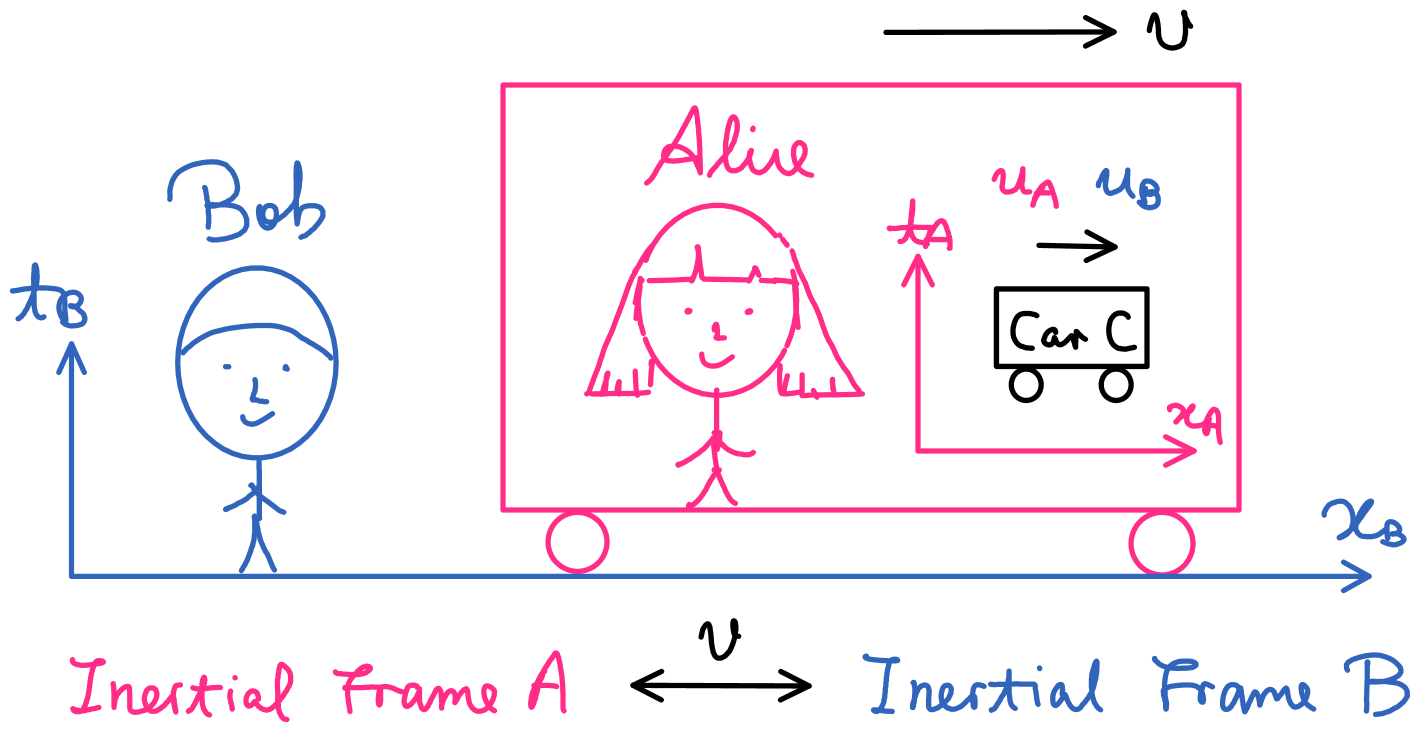
\includegraphics[width=0.7\textwidth]{galileo_relativity}
	\caption{\label{fig:grel} 王二有他的时间 $t_A$ 和空间 $x_A$;王三也有他的时间 $t_B$ 和空间坐标$x_B$。 王三和王二的相对速度为 $v$(因为王二站在一辆移动的大车上)。一辆小型汽车 C 的速度相对于王二为 $u_A$ ,相比于王三为 $u_B$。为简单起见,我们只展示$x$方向上的运动,而不考虑其他空间维度 $y$ 和 $z$ 的运动。}
\end{figure} 

\mtextbox{伽利略的理论是简单而微不足道的吗?}{
		现在$(\mathbb{R})$看起来很简单。 这是因为我们已经学习了牛顿力学。 
		\mnewline
	但在伽利略(1564-1642)时代,人们还没有加速度的概念,他靠肉眼来进行天文学的探索。当时的人们更相信地心模型而不是日心说(地球围绕太阳运动)。 地心模型的一个论点是,如果地球移动得很快,我们就会从地球上掉下来,而 $(\mathbb{R})$ 表明它不会发生。
		\mnewline
此外,现在我们还知道 $(\mathbb{R})$在牛顿力学不成立的情况下仍然成立,包括在狭义相对论成立的时候以及其他的一些情况。}
\textbox{伽利略的相对性原理}{
	物理定律在所有惯性系中都是相同的 \index{伽利略的相对性原理}
	\tcblower
因为会多次提到伽利略的相对性原理,所以在此让我们把伽利略的相对性原理简写为 $(\mathbb{R})$ 。这里有一些和$(\mathbb{R})$等效的语句:
	\titem{
		\item 运动是相对的。
		\item 没有绝对意义上的“运动”。
	}
我们把从一个惯性系到另一个惯性系通过相对运动的变化,称为“推动”变换。因此我们也可以说
\titem{
		\item 定律不会因“推动”变换,即惯性系的不同而改变。
	}
}

\textbox{牛顿力学和伽利略相对论的一致性}{
在 图~\ref{fig:grel} 中,牛顿第二定律(物理定律)对于王三和王二是否是相同的? 要证明这一点,请注意参考系之间的关系是	\begin{align}\label{eq:newtontx}
		t_B = t_A~, \qquad
		x_B = x_A + v t_A~.
	\end{align}
	王二参考系中的牛二定律是 $F = m a_A$。 那么在王三的参考系中呢?王三选取王二 的方程并将其转换为用王三参考系中的物理量表示:\marginnote{符号表示: $\dot x \equiv dx/dt$, $\ddot x \equiv d^2x/dt^2$. 
	\mnewline
你能尝试验证牛顿第一定律和第三定律吗?}
	\begin{align}
		F = m a_A = m \ddot{x}_A = m \ddot{x}_B = m a_B~.
	\end{align}
因此,王二在他的坐标系中确实具有相同的牛二定律。

以便以后的使用,我们总结出牛顿力学中的速度相加规则可以从同一个坐标系变换 \eqref{eq:newtontx} 导出:	\begin{align}
		\label{eq:vel_add_newton} 
		u_A = \dot x_A~,
		\qquad
		u_B = \dot x_B = u_A + v~. 	  
	\end{align}
}

从上文中,我们发现: $(\mathbb{R})$ 和牛顿力学可以得出相同的结果。 然而,牛顿力学并不是唯一满足 $(\mathbb{R})$ 的体系。 为了更好的说明这一点,并引出爱因斯坦的相对论,让我们先来介绍另一个基本的物理现象。

\subsection{光的速度}

\mtextbox{(拓展内容) 对于光速有限的观测}{
	早在 1676 年,R{\o}mer 就注意到实际观测到的木星卫星 Io 的日食在发生在地球L、K、G 和 F 位置时与计算的时间存在差异。这被解释为 : 光需要时间穿过 LK 和 GF 区间。
	\newline
	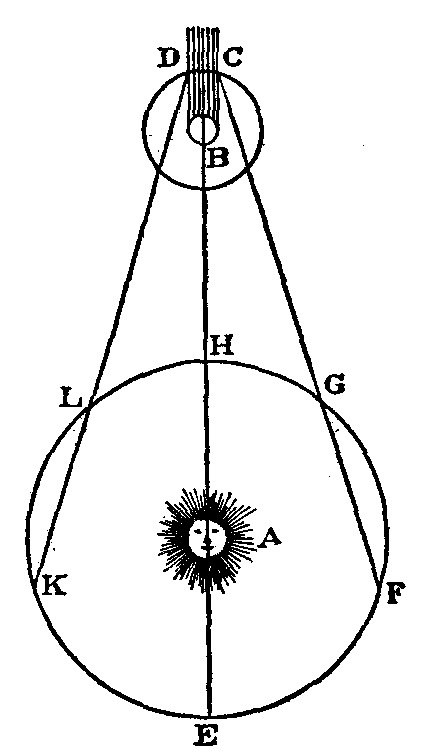
\includegraphics[width=\textwidth]{Romer_light}
} 

当我们打开灯时,光线“立即”充满了整个房间。在我们的日常生活中,光速是如此之快,以至于我们通常会忽略光所需的传播时间。 然而,光速是究竟是无限的,还是有限的呢?

科学家们设计了很多精细的实验来证明光速实际上是有限的,光的速度大约是 $c\simeq 3\times 10^8 $m/s。 右侧方框概述了天文学的第一个观察结果。 如今,光速的有限性不仅成为了现代物理的事实,而且在未来的应用中也有着巨大的前景。

\textbox{光速的精确值}{ \index{光速}
	光速 $c$ 有一个精确的值: $c = 299,792,458\mbox{m/s}$. 
	
这个事实是不是让你感到了惊讶? 通常,物理常数是通过测量确定的。 测量总是有误差的。 那么,$c$ 怎么会有一个准确的值呢?	
	\tcblower
	
米的现代定义(自 1983 年以来)是光在 1 秒内传播的距离(也就是$c$ 的值)。 事实上,在历史上(1889-1960)米是由一个被称为“国际原型米”的真实物体定义的。 但是使用真实物体定义仪表有很多缺点,包括	\titem{
		\item 人们必须与原型(或它的副本)进行比较以确定长度。
		\item 副本的准确性受到当时技术的限制。
		\item 原型的长度随时间略有变化。 甚至它可能会损坏。
	}
通过使用自然常数 $c$ 来定义米的概念,所有人都可以得到一米的长度。 误差仅受他/她实验精度的限制。 此外,时间和质量的现代定义也使用了量子力学的基本性质,它们是通过原子频率和普朗克常数定义的。}

现在,让我们来到这一节的重点,也就是爱因斯坦狭义相对论的基石。

\marginnote{我们已经说过光速是在现代定义长度的一种方式。 但是现在,让我们先回到 1900 年代初期,人们仍然考虑以单位时间内移动的距离来衡量的光速,以及距离和时间符合常识的定义。}
\textbox{来自移动光源的光的速度是多少?}{
	王三拿着蜡烛。 王三蜡烛发出的光相对于王三的速度是 $c_3 = c$ 。 
	王二在一辆车里以相对于王三 $v$ 的速度运动。 王二也拿着一个蜡烛,我们来思考:
	\titem{
		\item 王二蜡烛发出的光相对于王二的速度$c_2$ 是多少?
		\item 王二蜡烛发出的光相对于王三的速度$c_3$ 是多少?(注:此处 $c_3$ 与上文 $c_3$ 代表的是不同光源相对于王三的速度)
	}

	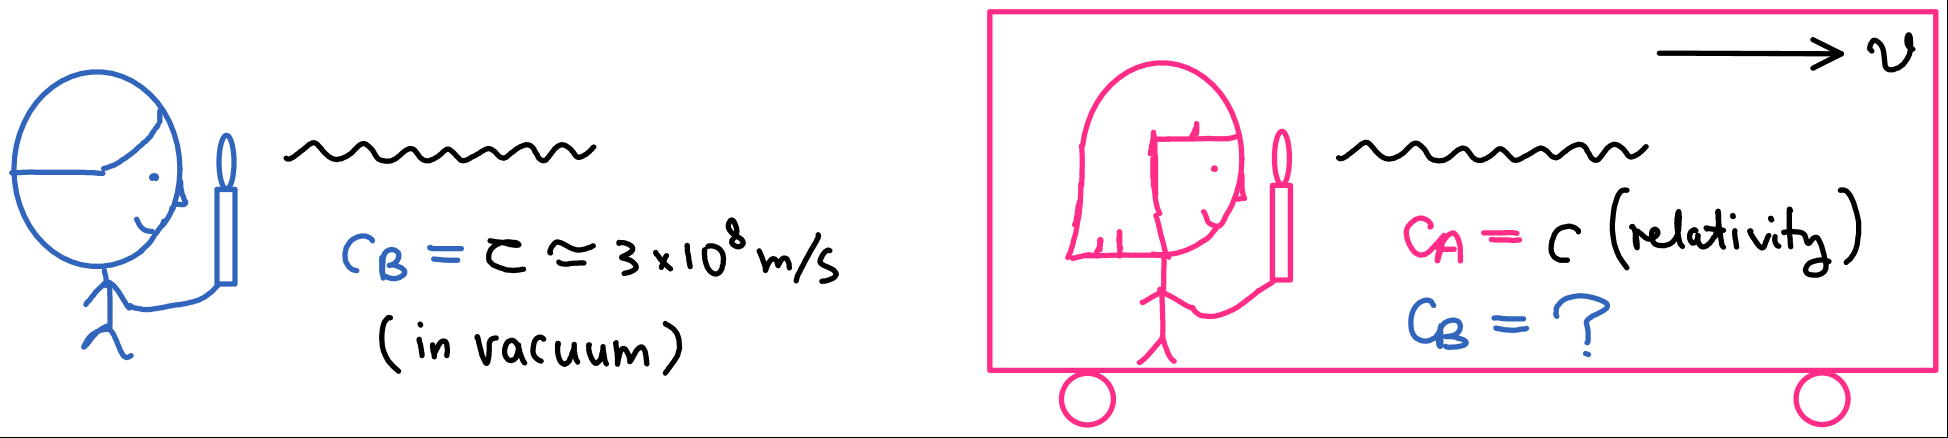
\includegraphics[width=0.6\textwidth, trim={0 3pt 3pt 0}, clip]{light}

	\tcblower

我们可以立即从 $(\mathbb{R})$ 得到 $c_A=c$。 否则王二就会通过测量到不同的光速值且不与汽车外部互动来知道他正在移动。 那么 $c_B$ 相对于王二的速度又是多少呢?}

我们可能会天真地得到 $c_B = c_A + v = c + v$ 通过牛顿力学中计算相对速度的原理。 \eqref{eq:vel_add_newton}. 而且这些看起来非常的正常 -- 在我们的日常生活中 (速度远小于光速): 如果王二在一辆相对于王三以速度 $v\ll c$ 运动的车里, 并相对王二自己以速度 $u_A$ 扔了一个球, 那么球相对于王三的速度就是 $u_B = v+u_A$.

然而,光传播的速度是由麦克斯韦方程推导出来的。 经过计算得到$c_B = c$! 下面的方框为您推导出了这个令人惊讶的事实。 推导需要使用多变量微积分,需要一些数学基础,因此,如果读者看不懂这些推导,您完全可以选择跳过它。

\mtextbox{麦克斯韦和相对论}{
事实上,隐藏在麦克斯韦方程组中的对称性已经暗示了爱因斯坦的狭义相对论。 光速不变只是其结果。 这种对称性被称为洛伦兹变换,是在爱因斯坦建立狭义相对论之前的 1887-1905 年间由 Voigt、Lorentz、Larmor 和 Poincare 提出的。 我们将在 \ref{sec:lorentz} 部分从机械的角度来讨论洛伦兹变换。}

\textbox{(拓展内容)由麦克斯韦方程组得出光速}{\index{speed of light from Maxwell equations}

	让我们来看王三的参考系。具有真空磁导率 $\mu_0$ 和介电常数 $\epsilon_0$ 的麦克斯韦方程为:

	\begin{minipage}{0.4\textwidth}
		\begin{align}
			\label{eq:mnde} \nabla \cdot  \mathbf{E} & = \frac{\rho}{\epsilon_0} ~,
		\end{align}
	\end{minipage}\hspace{0.1\textwidth}
	\begin{minipage}{0.45\textwidth}
		\begin{align}
			\label{eq:mndb}  \nabla \cdot  \mathbf{B} & = 0 ~,
		\end{align}
	\end{minipage}
	
	\begin{minipage}
		{0.4\textwidth}
		\begin{align}
			\label{eq:mnte} \nabla \times \mathbf{E} &= -\frac{\partial \mathbf{B}}{\partial t} ~,
		\end{align}
	\end{minipage}\hspace{0.1\textwidth}
	\begin{minipage}
		{0.45\textwidth}
		\begin{align}
			\label{eq:mntb} \nabla \times \mathbf{B} &= \mu_0 \left [ \mathbf{J} + \epsilon_0 \frac{\partial \mathbf{E}}{\partial t} \right ]~.
		\end{align}
	\end{minipage}\medskip

当我们研究光的传播时,我们考虑真空环境下的麦克斯韦方程。 因此电荷密度$\rho=0$,电流$\mathbf{J}=0$。 为了消除 $\mathbf{E}$ 并仅获得 $\mathbf{B}$ 的方程,我们使用以下技巧:让我们将\eqref{eq:mntb}的左边和右边同时进行$\nabla\times (\cdots)$ 的运算 ,得到:

	\begin{align} \nonumber
		\nabla\times\mbox{LHS} = \nabla\times(\nabla\times \mathbf{B})
		\xlongequal{\mbox{math identity}} \nabla (\nabla\cdot \mathbf{B}) - \nabla^2 \mathbf{B} \xlongequal{\mbox{using Eq.~\eqref{eq:mndb}}}
		- \nabla^2 \mathbf{B} ~,
	\end{align} 
	\begin{align} \nonumber
		\nabla\times\mbox{RHS} =  \mu_0\epsilon_0 \frac{\partial}{\partial t} (\nabla \times \mathbf{E}) 
		\xlongequal{\mbox{using Eq.~\eqref{eq:mnte}}} -\mu_0\epsilon_0 \frac{\partial^2}{\partial t^2} \mathbf{B} ~.
	\end{align}
	\mtextbox{相速度}{相速度可以从 \eqref{eq:maxwell_wave} 中的相位因子 $\cos[k(x-ct)]$ 得到。 这可以通过分析下图中的一个振荡周期来完成,我们来看看它是如何进行的。
		\\
		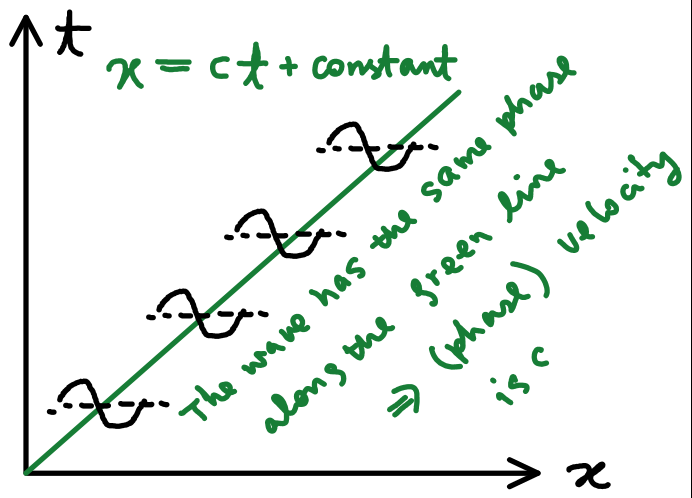
\includegraphics[width=\textwidth, trim={0 2pt 2pt 0}, clip]{phase_velocity}
		\\
	我们将在本课程后面的量子力学中遇到类似的波动方程,并使用复数解 $\exp[ik(x-ct)]$。 因此,一定要明白为什么 \eqref{eq:maxwell_wave} 描述的是一个移动的波。
		\mnewline
如果从更深层次思考,上述相速度实际上并不是描述信息传播速度的方式。 然后我们需要更谨慎地求解麦克斯韦方程组,并找到一个由加速源产生的解,然而这超出了当前讨论的范围。}
	因此, 左边=右边是一个波动方程:
	\begin{align}
		\label{eq:maxwell_wave}
		\frac{\partial^2}{\partial t^2} \mathbf{B} 
		- \frac{1}{\mu_0\epsilon_0} \nabla^2 \mathbf{B} = 0~. 
	\end{align}
	
	
	在数学物理方法的课程中, 我们会研究如何系统地求解这个方程。 但在这里我们不会这样做,相反的,我们可以给出一个解并检查它是否确实满足了 Eq.~\eqref{eq:maxwell_wave} 而无需运用更多数学知识。 我们可以检查一下以下的电磁 波是否是方程的解:
	\begin{align}
		\label{eq:sol_maxwell_wave}	B_z = B_0 \cos [k (x - ct) ]~,
		\qquad \mbox{where~} c \equiv \frac{1}{\sqrt{\mu_0\epsilon_0}} ~.
	\end{align}
计算得出的结论是:一旦发射一束电磁波,它就可以在真空中传播而无需发射器的参考,即发射器的运动信息被“遗忘”。 光速由自然常数 $\mu_0$ 和 $\epsilon_0$ 计算,与发射器(或观察者)的速度无关。 因此我们得出结论,答案是 $c_3=c$,与王二观察到的速度相同(即 $c_3=c_2$)!}

此刻一定有什么大错特错了:速度相加规则\eqref{eq:vel_add_newton}与独立于观察者的光速\eqref{eq:sol_maxwell_wave}不一致。 在这种情况下,我们需要通过实验来判断谁是对的。 迈克尔逊-莫雷干涉仪实验(1887 年)表明麦克斯韦是正确的。 牛顿力学的速度相加法则不适用于光!
\needspace{.1\textheight}
\mtextbox{近代的干涉仪}{
迈克尔逊-莫雷干涉仪旨在测量光速的变化。现在我们知道(至少可以假设)光速确实是一个常数,一个干涉仪可以通过调节干涉臂长度来实现精确测量。它在近代物理和近代计量技术中都有着重要的应用。}

\textbox{迈克尔逊-莫雷实验}{\index{迈克尔逊-莫雷干涉仪}
	\begin{minipage}
		{0.45\textwidth}
		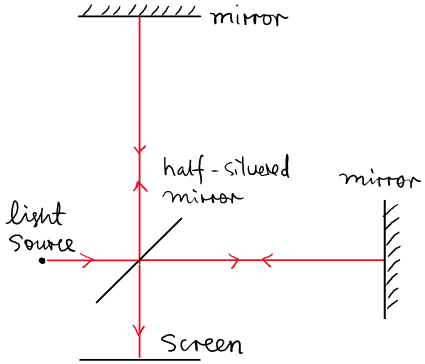
\includegraphics[width=\textwidth]{mm-experiment}
	\end{minipage}\hspace{0.04\textwidth}
	\begin{minipage}
		{0.5\textwidth} 一束光从光源发出,通过半镀银镜(分光镜),光束被分成两束,分别被两个镜子反射到屏幕上。由于光程不同,会产生干涉条纹。
		
请注意,该实验是在地球上进行的。 地球以 $v\sim 30 $km/s 的速度围绕太阳运动。 因此,如果牛顿力学的速度相加规则适用,迈克尔逊-莫雷干涉仪中的光速应该随着旋转而变化,然后干涉条纹应该移动。 但是没有观察到这种变换,因此速度没有增加。 因此麦克斯韦的理论战胜了牛顿的理论。	\end{minipage}
}

\mtextbox{是牛顿错了吗?}{
既然速度加法(在牛顿力学的核心)对光无效,牛顿错了吗? 我们应该放弃牛顿力学吗?	\mnewline
在现代物理学中,我们认为大多数理论都是“有效的”理论——它们适用于某些近似值。 当 $v\ll c$ 时,牛顿力学仍然有用,因为它非常精确,而且比狭义相对论更简单、更直观。	\mnewline
因此,学习狭义相对论并不是要我们要放弃牛顿力学。 相反,在现代,牛顿力学仍然比狭义相对论使用的更广泛(因为我们通常不以 $v\sim c$ 移动或考虑受 $v/c$ 影响的修正)。
\mnewline
事实上,狭义相对论也有类似的命运——它是经典的。 当考虑非常小的粒子时,必须考虑量子力学,我们得出了量子场论。 而考虑到引力的量子效应,量子场论又是远远不够的……}
\textbox{选读的历史内容: 以太的故事}{\index{aether}
	事实上,我们在这里介绍的不是研究人员在 100 年前做出这些发现时的想法。

在麦克斯韦时代,人们认为电磁波在称为以太的介质中传播,类似于在空气中传播的声波。 因此,光速 $c=1/\sqrt{\mu_0\epsilon_0}$ 也是相对于以太而言。 参数 $\mu_0$ 和 $\epsilon_0$ 被认为是以太的属性,而不是真空的属性。	
既然如此,速度相加规则就没有问题了——就像风的速度和声波在风中传播的速度相加一样。
现在的问题是:当地球绕太阳公转时,地球周围的以太是与地球一起运动的,还是保持静止的?
对恒星畸变(1600s - 1700s)的观察表明,以太不与地球一起运动。 在以太的背景下,迈克尔逊-莫雷实验表明以太确实与地球一起移动。 这是100年前困扰物理学家的问题。 而爱因斯坦的贡献是用他的相对论消除了对以太的需要。
由于以太的理论被废弃,现在我们学习电磁波时,我们不再介绍以太,我们选择用更接近现代思维的介绍方式,而不是历史思维,因此我们只在这个这里留下一个关于以太的评论。}

\subsection{爱因斯坦的相对论}

我们如何化解麦克斯韦独立于观察者的$c$与速度加法规则之间的矛盾呢? 这是20世纪初物理学的两大难题之一。 

爱因斯坦 16 岁时,就已经对光产生了深深的困惑:如果我跑得像光一样快怎么办? 光会静止吗? 10年后,他找到了解决办法。

以下是爱因斯坦在 1905 年解决这个问题的方法:他将 $c$ 相对于观察者的独立性作为他理论的基本假设。于是问题解决了:
)

每个人都可以做出假设,但真正具有革命性的是假设的含义以及如何在此基础上获得统一的理论。为了更清晰的理解爱因斯坦的理论,我们在这里总结了假设,并进行更深入的研究。
 
\mtextbox{Remarks about ($\mathbb{C}$)}{
	\mtitem{
		\item 光的速率与观察者无关,但并不是说与速度无关。换句话说,光的方向可以取决于观察者。稍后我们将在讲到“光钟”时清楚地看到这一点。

		\item 光的频率取决于观察者(相对论多普勒效应)。当你向光移动时,光频率会变高(蓝移)。当你远离光时,光频率变低(红移)。

		\item 在非真空情况下,光速将取决于介质的运动。稍后可以使用相对论速度相加规则来获得介质中移动坐标系的光速。
 
	}
}
\itembox{狭义相对论的基本假设}{}{\index{狭义相对论的基本假设}
	\item ($\mathbb{R}$) 相对性原理:物理定律在所有惯性系中都是相同的。

	\item ($\mathbb{C}$) 在在所有惯性系中,真空光速为 $c$。

} 

 ($\mathbb{R}$) 和 ($\mathbb{C}$)是狭义相对论中的基本假设。但要明确的是,还必须假设事件观察者的独立性才能满足狭义相对论理论的基本要求:


\textbox{独立于观察者的事件假设}{\index{事件}
	($\mathbb{E}$) 
	让我们考虑一个在特定时刻发生在一个特定小物体上的事件 (在时空坐标中确定的一点),事件发生(或不发生)与观察者无关。如果一个观察者发现事件 E 发生了,那么所有看到该事件的观察者都必须观察到(同意)此事件发生了,无论他们是如何移动的。

	
	\tcblower
	
	尽管这个假设看起来非常的微不足道,但还是让我们把事情说清楚。

例如,以下是所有(诚实的)观察者必须同意的事件:

	\titem{
		\item ``一束光被镜子反射''
		\item ``王一和王二见面了。见面的时候,他们的手表都指向了上午10点。''
	}
以下这些就不是事件:
	\mtextbox{不是一个事件,而是两个事件的情况}{在王二和王三相隔5光年的例子中,这句话不是一个事件,但可以把它分成两个事件:当王二看她的手表时,她的手表显示上午10点。当王三看他的手表时,他的手表显示的是上午10点。这同样适用于标尺示例的比较。讨论相对论中事件的关系是有道理的,我们将在后面看到。}
	\titem{
		\item ``王二和王三相距5 光年。当王二的手表指向上午 10 点时,王三的手表也指向了上午 10 点。''
	}
这不是事件,因为 Alice 和 Bob 在不同的位置。因此,观察者查理可能会认为上述陈述是正确的;而另一个运动的观察者却认为上述说法是错误的。

同样,以下内容也不是事件,或许所有的观察者都不认可这种陈述:
	\titem{
		\item ``移动的尺子与静态的尺子具有相同的长度,因为两个端点同时重合。''
	}
}

\textbox{注:事件相对于某个参考系发生的时间}{
由于光速有限,我们需要讲清楚事件发生的时间。例如,事件发生在距离鲍勃一定距离的地方。在谈到事件的时间时,它可以指:

	\marginnote{
		我们说在每一个空间点上的钟指的是: 钟相对于bob静止并且和bob的坐标系是完全同步的, (他坐标系中的时间). 同步时钟可以通过比较光信号, 并减去用于光传播的时间来完成。
		\\
		“观察”或者“记录”的意思是假设 Bob在他的参考系中的每个点都有一个助手。一旦发生任何事件,助手可以立即记下 Bob 的时间和事件的空间坐标。这将由事件 $(t_B, x_B)$相对于Bob的坐标表示。}
	\titem{ 
		\item Bob 参考系中的时间。想象一下,鲍勃在他的框架中的每个空间点都放了一个时钟,它“观察”到了事件发生的时间。

		\item Bob 实际“看到”事件的时间。这需要占用事件和 Bob 之间的光传播时间。
	}
	在本课程中,当谈论 Bob 的时间时,除非另外强调,否则我们将默认使用 Bob 参考系中的时间,而不是 Bob 实际看到到达他的事件的光信号的时间。

}

有了这三个假设,我们现在准备开始狭义相对论的旅程。


\section{时间膨胀(钟慢效应)}\label{sec:time-dilation}

在这部分的开头,我们承诺了读者会在后文解释为什么太空旅行者爱丽丝回来时比鲍勃年轻(如果她在太空旅行前最初与鲍勃年龄相同)。探寻清楚这个问题这就是本节的目标。

为此,我们必须提及到物理学中最基本的概念——时间。首先,让我们回顾一下牛顿是如何评论时间的。

    \mtextbox{我们可以相信的什么?}{
    现在我们要超越牛顿,你可能想知道,我们能相信牛顿理论的什么。我们当然想站在牛顿的肩膀上把他的一些遗产物尽其用。
	\tcblower
    几乎所有低速运动($v\ll c$),牛顿力学的结果都是可信的(除了静止能量,我们将在后面讨论)。对于高速运动 ($v\sim c$),我们只相信 $(\mathbb R)$、$(\mathbb C)$、$(\mathbb E)$ 。

	\mnewline
    例如,在讨论时间时:我们相信爱丽丝的机械表(静态的爱丽丝)很好地定义了爱丽丝的时间,因为机械表的时间是低速机械运动的结果。但是我们不能相信牛顿理论中关于爱丽丝的时间(由她的机械表的转动来定义)如何在鲍勃身上流逝的结论,如果鲍勃相对于爱丽丝有 $v\sim c$ 的相对运动。在讨论长度时:我们相信爱丽丝的尺子(静态的爱丽丝)定义了爱丽丝的长度,但我们不能相信鲍勃如何观察爱丽丝的尺子的长度。
}
\textbox{牛顿理论中的时间}{\index{牛顿理论中的时间}
	``绝对的、真实的和数学的时间,它本身,从它的本性出发,平等地流动,不考虑任何外部的东西,另外一个名字叫做持续时间:相对的、明显的和普通的时间,是一些合理的和外部的(无论是准确的还是不公平的) ) 通过运动来测量持续时间,通常用于代替真实时间'' 
	-- 牛顿《自然哲学的数学原理》
	\tcblower

因此,牛顿相信“真实时间”独立于任何其他事物而存在。如果是这样,怎样才可以测量真实时间呢?

	\titem{
		\item 如果我们无法得到它, 那我们为什么要耗费精力去定义“真实时间”呢? 我们为什么不直接摒弃这个概念呢?
		\item 如果它可以被一个设备测量出来,那为什么它不能被这个设备改变呢?我们想一想牛顿第三定律,当真实时间对装置产生某种作用时,为什么装置不能对真实时间进行反向的作用并改变它呢?

	}
}

我们是物理学家。我们可以做些什么来摆脱关于时间的形而上学思维呢?我们来做一件实际的事情——通过实际制作一个最简单的时钟来定义时间:光钟。

\textbox{制作光钟}{\index{光钟}
	\begin{minipage}
		{0.45\textwidth}
		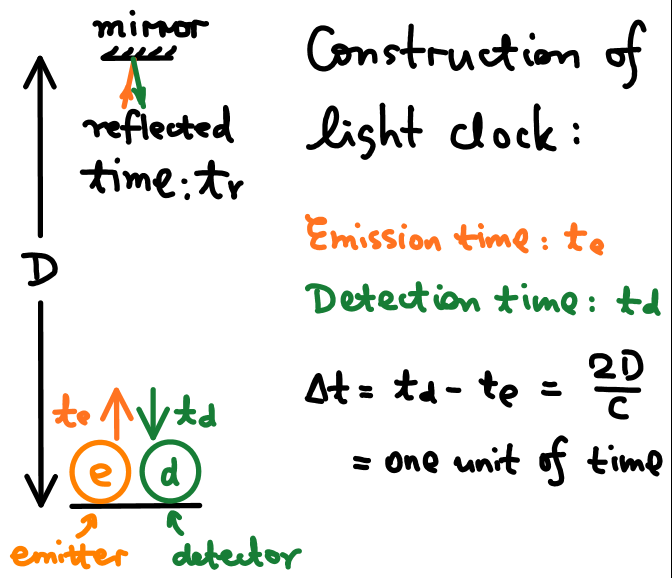
\includegraphics[width=\textwidth, trim={0 3pt 3pt 0}, clip]{light_clock}
	\end{minipage}\hspace{0.04\textwidth}
	\begin{minipage}
		{0.51\textwidth}我们用光钟的滴答声来定义时间间隔。 滴答时间间隔 $\Delta t$ 是发射器发射光(时间 $t_e$)和检测器检测到光(时间 $t_d$)之间的时间。在过程中,光被镜子反射(在时间 $t_r$)。
对于光钟,“标准时间间隔”可以定义为 \marginnote{发射器和检测器放在一起,它们非常接近,我们可以认为在同一点上(在图中它们分开绘制只是为了表示清楚)。}
		\begin{align}
			\label{eq:time_interval}
			\Delta t \equiv t_d - t_e = \frac{2D}{c}~. 
		\end{align}

		于是我们就可以通过两个事件之间的“标准时间间隔”的数量来测量时间了。
	\end{minipage}
}

为了了解旅行者的时间相比于静态观察者如何,我们把光钟放到爱丽丝的车上。

\textbox{把光钟放到爱丽丝的车上}{
	\begin{minipage} 
		{0.6\textwidth}
		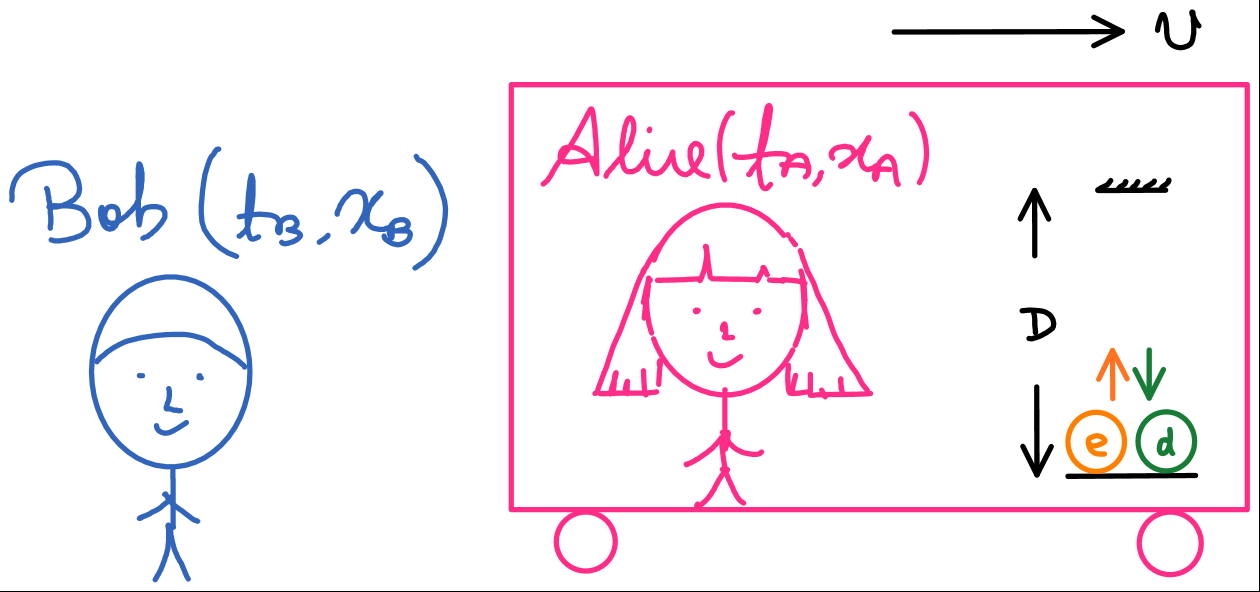
\includegraphics[width=\textwidth, trim={0 3pt 3pt 0}, clip]{light_clock_car}
	\end{minipage}\hspace{0.04\textwidth}
	\begin{minipage}
		{0.36\textwidth} 
		To 
		\marginnote{这里我们假设光钟离爱丽丝足够近,在爱丽丝的参考下,她自己和时钟的空间坐标都是 $x_A=0$。}
        现在让我们与爱丽丝一起将光钟装入汽车,看看旅行者的时间流逝与静态观察者相比如何。根据 ($\mathbb{R}$),Alice 发现光钟的间隔是 $\Delta t_A = 2D/c$。

现在我们需要找出 $\Delta t_B$ 并将其与 $\Delta t_A$ 进行比较。
	\end{minipage}	
}

\needspace{.25\textheight}
\mtextbox{相同的垂直长度}{
	此时你可能有一个很好的问题:当光钟在移动时,我们怎么知道光钟的长度相比于Bob仍然是 $D$ ?

	\tcblower
	考虑一个思想实验:火车在轨道上。列车静止时,其车轮的间距与轨道宽度相同。现在火车开得很快。与轨道相比,它的轮子的宽度是更大还是更小?两者都不。否则就会发生与 ($\mathbb{E}$) 矛盾的事故。

}
\textbox{鲍勃测量的爱丽丝光钟的时间间隔}{
	\begin{minipage}
		{0.55\textwidth}
		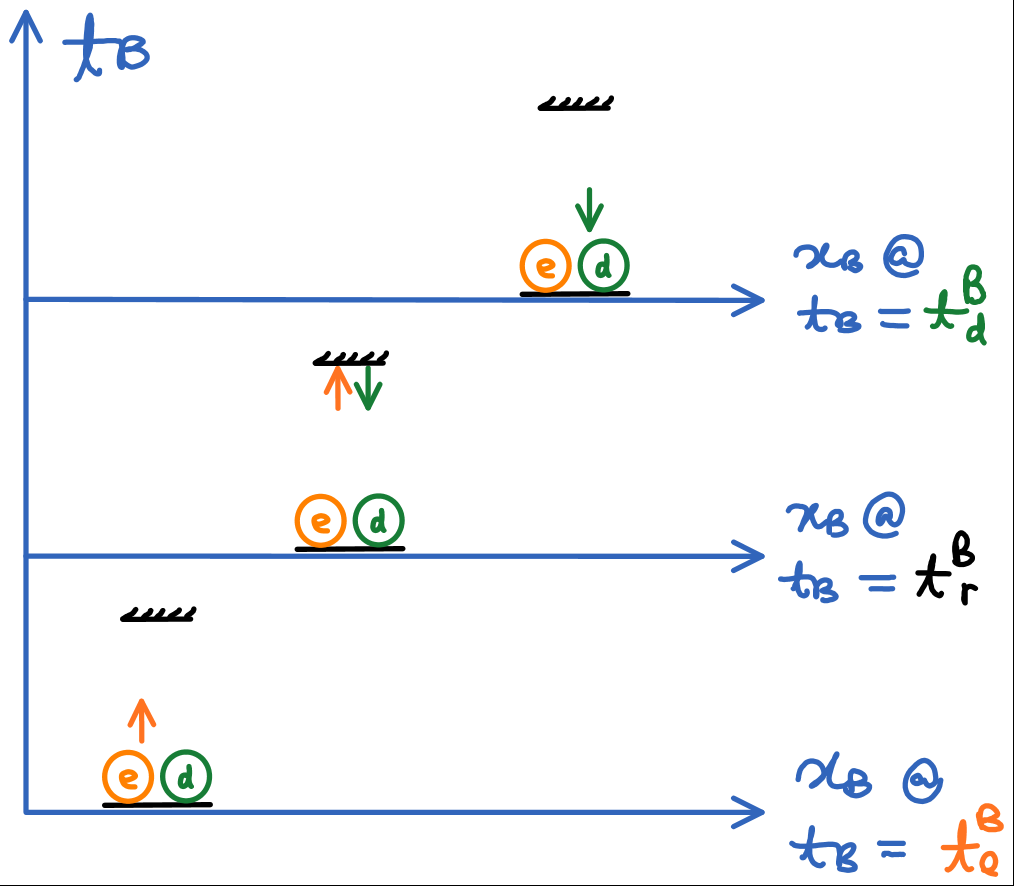
\includegraphics[width=\textwidth, trim={0 2pt 2pt 0}, clip]{light_clock_B}
	\end{minipage}
	\hspace{0.05\textwidth}
	\begin{minipage}
		{0.4\textwidth}
		左图是鲍勃对移动时钟的看法。这里 $x_B$ 和 $t_B$ 分别是鲍勃的空间和时间。
		
		我们拍摄了三个时间快照:在 $t_B = t_d^B$ 处的信号发射,光被镜子反射的时间 $t_B = t_r^B$,以及光被接收器接收的时间 $ t_B=t_d^B$。

        光钟的位置和状态如图。
	\end{minipage}

	\bigskip

	\begin{minipage}
		{0.35\textwidth}
		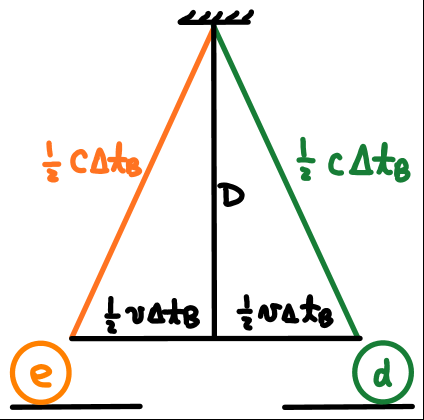
\includegraphics[width=\textwidth, trim={0 2pt 2pt 0}, clip]{light_clock_B1}
	\end{minipage}
	\hspace{0.05\textwidth}
	\begin{minipage}
		{0.6\textwidth}
		在左图中,我们绘制了 Bob 的移动光钟中的光轨迹。鲍勃一定认可光线击中了镜子 ($\mathbb{E}$)。因此光的方向必须不再是垂直的。并且从($\mathbb{C}$),从发射器到镜子的光速仍然是$c$。

		
		根据勾股定理,我们有
		\begin{align}
			\label{eq:lcb}
			\left ( \frac{1}{2} c \Delta t_B \right )^2 = \left ( \frac{1}{2} v \Delta t_B \right )^2 + D^2 ~,
		\end{align}
	\end{minipage}

	\bigskip

	\tcblower
	
	因此,我们可以求解 $\Delta t_B$ -- Bob测量的Alice的时间间隔:

	\begin{align}
		\label{eq:dtb}
		\Delta t_B = \frac{2D}{c} \frac{1}{\sqrt{1-\frac{v^2}{c^2} }} = \gamma \Delta t_A ~,
		\qquad
		\gamma \equiv \frac{1}{\sqrt{1-\frac{v^2}{c^2} }} > 1~.
	\end{align}
	因此,在王三的参考系中,王二的光钟变慢了。这也被称为移动时钟的“时间膨胀”(也就是动钟变慢)。
}

\textbox{不仅是王二的光钟,整个王二参考系相对于王三都变慢了
}{
	在这时, 
	\marginnote{``你的钟如何与我无关。我在乎的是你呀。'' -- 王三}
	我们说王二的一切相对于王三都减慢了是不够有说服力的。 因为我们只是说明了她的光钟变慢了。 那么她的闹钟,手机,心率又是怎么样的呢?

	\mtextbox{和绝对时间说再见吧}{通过“动钟变慢”,人们注意到牛顿的“绝对时间”概念随着速度而消失。 不同的搬运工有不同的时间; 没有绝对的推动者,因此也没有绝对的时间。
	\\
	我们在稍后以及在学习到广义相对论章节时还会回到}

	\tcblower

	事实上,根据 ($\mathbb{R}$),上述的一切都变慢了。

	假如 Alice 有一个手机,它可以定义单位时间间隔。 她把光钟和手机放在非常靠近的地方。 如果手机和光钟在静止参考系中具有相同的 $\Delta t$,则它们必须具有与 Alice ($\mathbb{R}$) 相同的 $\Delta t_A$。 他们的共识是一个事件,Bob 必须同意 ($\mathbb{E}$)。 因此鲍勃必须同意手机与光时钟定义的 $\Delta t_B$ 是相同的。
}

\textbox{狭义相对论中的总结和四步推理}{\index{时间膨胀}\index{四步推理}
	我希望现在你已经明白为什么太空旅行者爱丽丝回来时比鲍勃年轻——作为一个移动的观察者,她相对于鲍勃变慢了。

	\mtextbox{ $\Delta t_B$的意义}{这里注意,$\Delta t_B$ 并不是 Bob 光钟的时间间隔,而是 Alice 的光钟(即与 Alice 一起移动)在 Bob 的参考系中的时间间隔。 所以说相对于鲍勃(静态观察者),爱丽丝的时间变慢了。}
	\tcblower

	推理的4个关键步骤很重要,我们将重复使用类似的方法。 因此,让我们在这里总结一下:
	\tenum{
		\item 在静静止参考系中构建仪器。 仪器应该尽可能简单,以便我们计算仪器内部实际发生的情况。 这里的装置是标准时间间隔$\Delta t = 2D/c$的光钟。
		\item 将装置放入爱丽丝的移动汽车。 根据 ($\mathbb{R}$) ,Alice的观察结果一定是设备运动与静止时的工作方式是相同的。 这里 Alice 发现 $\Delta t_A = \Delta t$。
		\item 计算鲍勃得到的结果,将结果与 Alice 得到的结果进行比较。 我们已经计算出 $\Delta t_B = \gamma \Delta t_A$。 因此,移动的光钟变慢了。
		\item 虽然结果是由一个特定的仪器获得的,但 Bob 的参考系和 Alice 的参考系之间的比较适用于所有的设备。 因为要不是这样,就可以使用这个差异来识别绝对运动的人了 ($\mathbb{R}$)。
	}
}

\textbox{参考系的时间以及Bob看到了什么}{
	\twocol{0.85}{0}{0.65}{
		我们已经提到了“参考系的时间”这个概念:如果没有另外说明,当我们提到时间时,我们指的是一个人参考系中的时间,而不是光进入观察者眼睛的时间。 现在让我们更清楚地说明这一点。

让我们在空间中的每个点(比如 $x$-方向)放置两个东西:
		\titem{
			\item 一个空间标记。 例如,假设沿 $x$ 方向有一个标尺,标尺的刻度就是空间标记。
			\item 一个钟。时钟在空间中的所有点都是同步的(有关如何同步时钟的信息,请参阅关于校对时钟的部分)。 
		}
		时间膨胀 ($\Delta t_B$) 的意思是,Alice 的时钟(标有 $\vec v$ 的红色时钟)在移动,下一时刻,它与 Bob 帧中的另一个时钟进行比较,并且它变慢了。在这个比较中,时间膨胀不取决于爱丽丝的车是向鲍勃运动还是远离鲍勃运动。

		Bob 实际“看到”的东西,用 $\Delta t_B^{\mbox{``see''}}$ 表示:由于光速是有限的,所以光会有延迟。光线从 Alice 的时钟传播到 Bob 的眼睛(红色波浪线)。 $\Delta t_B^{\mbox{``see''}}$ 取决于爱丽丝是向鲍勃运动还是远离鲍勃运动。
	}{
		\cg{0.9}{frame_meaning}
	}	
}

    既然你已经了解了时间膨胀以及为什么太空旅行者爱丽丝更年轻。 那么现在就是再次把你搞糊涂你的好时机,让我们来看看著名的“双生子佯谬”。

\needspace{0.4\textwidth}
\mtextbox{时空旅行?}{
	双生子佯谬是时间旅行到未来的一个例子。 如果你乘坐宇宙飞船旅行并返回,你就会到达未来。 如果太空旅行足够快,往返在1年之内,你就可以看到下个世纪,甚至更晚的地球。 在广义相对论中,我们将看到更多前往未来的方式,例如靠近黑洞。
	\mnewline
	穿越到过去呢? 一会我们就会发现狭义相对论是如何防止通过时间旅行回到过去的。 还有比较普遍的问题,比如穿越到过去,不让爸爸妈妈见面会怎么样? 如果你穿越到过去,遇到另一个自己怎么办?  穿越到过去大概是不可能的,虽然此刻我们还无法做出决定性的结论。
}
\textbox{谁在运动?到底谁更年轻呢? -- 双生子佯谬}{\index{双生子佯谬}
	我们已经证明:Bob 发现 Alice 更年轻(根据他参考系中的时钟)。 然而,运动是相对的($\mathbb{R}$)。 因此,爱丽丝不也应该发现鲍勃更年轻吗?

	\tcblower

	让我们通过两个步骤来解决这个问题:
	\tenum{
		\item Alice 和Bob的参考系都是惯性系,它们一直有相对运动。 根据 ($\mathbb{R}$),“Alice 认为 Bob 更年轻”和“Bob 认为 Alice 更年轻”都是正确的。

		乍一看,这与 ($\mathbb{E}$) 矛盾,但实际上并不矛盾。 作为匀速运动的人,爱丽丝和鲍勃只能见面一次。 这是一开始 Alice 与 Bob 年龄相同的时间,后来他们再也没有见面。 因此,没有本地事件来比较他们的年龄(使用 \emph{events} 比较 $\Delta t_B$ 和 $\Delta t_A$,它们必须至少相遇两次)。

		\item 爱丽丝先运动,然后折反回来见到鲍勃。 这与我们在本部分的开始讨论的设置相同。

		我们目前只能相信鲍勃。这是因为Alice要折返,这段时间Alice不在惯性系中。 相对性原理(我们在得出结论时使用了很多次)不适用于非惯性观察者。 因此,我们只能相信 Bob 的观点,即 Alice 更年轻。
	}
}

\section{物理图像和物理直觉}\label{sec:phys-pict}

本节无关物理的理论知识。考虑到现代物理学与经典物理学如此不同,停下来讨论学习方法是很重要的。  我们选择把这个部分放在这里而不是最开始(尽管这在逻辑上更合理),是因为在没有任何现代物理的实际经验之前,谈论这些是空洞的。

\textbox{为什么现代物理不同于经典物理(即普通物理)?}{
	从狭义相对论的时间膨胀,你已经初步接触了现代物理学的一点理论。 如果你还没有学过它,你一定会觉得它是违反直觉的,比普通物理的绝大多数部分更令人困惑。

	之后还要更多现代物理的理论——你将了解更多关于相对论、引力、量子、信息、复杂性的知识……面前是一个全新的世界。 这些主题的共同特点不仅是它们是在大约过去100年才被发现的,而且它们离我们的日常经验更远。 这就与是经典物理学的不同之处。

	不要被这些吓到!这就是这一节存在的原因。

	\tcblower

	顺便说一下,数学、文学和艺术也有类似的过渡——它们也从古典演变到现代。 文学、艺术、数学和物理的现代化革命固然不同,但有着有趣的相似之处。
}

让我们用一个练习来谈谈思考的方法,以及学习现代物理值得推荐的方法。

\textbox{小练习}{
	一枚“手榴弹”
     \marginnote{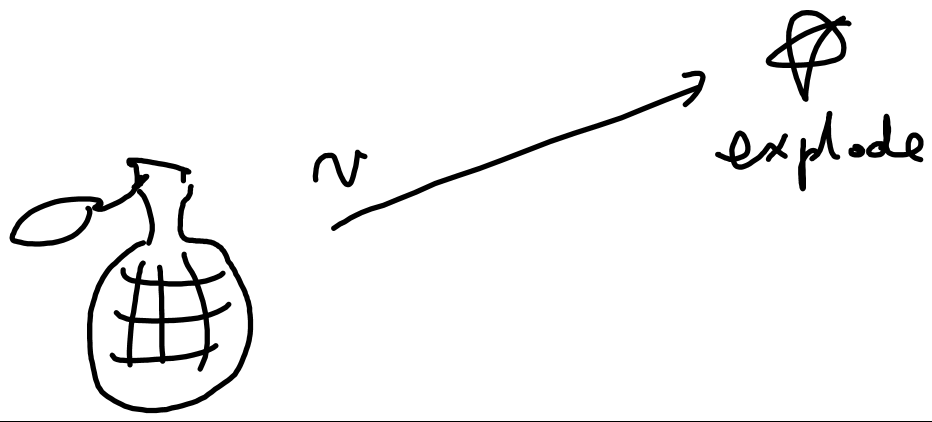
\includegraphics[width=0.3\textwidth, trim={0 2pt 2pt 0}, clip]{grenade}}
是一种在触发后一定时间爆炸的炸弹。 设手榴弹静止时触发到爆炸的时间间隔为$\Delta t$。 现在你以 $v$ 的速度扔手榴弹。 计算狭义相对论理论下手榴弹爆炸前运动的距离。 在计算中,地球重力和空气摩擦都可以忽略。
	
	\tcblower

	在解决这个问题之前,让我们讨论 3 种“思考”如何解决它的方法(\emph{不是} 三种解决方法)。

	\titem{
		\item \emph{配对}。 将问题配对(转换)为已解决的问题: "Bob" $\leftrightarrow$ "你"; "爱丽丝" $\leftrightarrow$ "手榴弹"; $\Delta t_A$ $\leftrightarrow$ $\Delta t$ 因此$v\Delta t_B = \gamma v \Delta t$ $\rightarrow$ $s$。
        \item \emph{反向推理}。 问距离,那么如何计算距离,速度给定,所以$s=v t$。 现在如何得到$t$? 哪个方程有 $t$? 这是一个关于相对论的问题,所以应该是 $\Delta t_B = \gamma \Delta t_A$(希望你得到 $\gamma$ 而不是 $1/\gamma$)。 因此,$s=\gamma v \Delta t$。
        \item \emph{实物图像}。 想象一下手榴弹飞出一段距离然后爆炸。 你看到了文字,但在你的脑海中播放了一段画面。 手榴弹的时间变慢了。 所以它必须比平时运行更长的时间,从而运行更长的距离。 飞行时间长了一个 $\gamma$ 因子,因此行进的距离长了一个 $\gamma$ 因子:$s = \gamma v \Delta t$。
	}
}

在准备考试时,我们可能主要使用第一种和第二种方法进行了大量培训。 但如果你想成为一名创新的物理学家,或者至少想成为一名物理学家,那么第三种思维方式是主要的方式。因为:

\itembox{为什么物理直觉和物理图像很重要}{}{
	\item 一张真实的图片可以将你学到的东西与现实世界联系起来,而其他两种方法不可以。在研究中,您需要了解该理论的可能应用,或者如何进行近似以简化分析。实物图片指导您做到这一点,而其他两个方法没有。 
\item 一张实物图片告诉你你的答案是否有意义。如果你在某个地方犯了错误,而你脑子里有一张实物图,那么你就有很好的机会尽早发现它。
\item 研究意味着模式匹配不会给你带来好的结果的新问题。 (但您确实必须使用模式匹配来确保您的想法是新的。)
\item 研究人员必须在解决问题之前定义问题(与已经明确定义的考试问题不同)。清晰的实物图片告诉您如何定义问题。反向搜索或模式匹配不能。
\item 作为一名研究人员,需要与人交谈。在大多数讨论中(尤其是那些没有黑板的讨论),你都是通过实物图片来说话的。
\item 计算机擅长模式匹配和反向搜索。人工智能的兴起更有可能降低你的模式匹配和逆向搜索工作的价值,但不太可能是基于直觉的工作。
}

我希望你现在确信:即使是物理学在现代也变得不那么直观了,你应该尝试通过建立物理图片来使其尽可能直观。这里有一些关于如何实现这一目标的建议。

\itembox{如何在现代物理学中建立物理图像/直觉?}{}{
\item 试着在你的脑海中“播放一部电影”来解决这个问题。在影片中包含尽可能多的相关物理细节。当你对某件事有新的理解时,把它加到“电影”中。
\item 当你发现一些不直观的东西时,请反复思考。你最终会对此感到更快乐。
\item 注意物理学中的悖论,以及它们是如何解决的。
\item 以不同的方式/角度思考同一个问题。
\item 与我们的日常生活经验进行比较。找出相似之处和/或关键差异。
\item 简化和模块化问题。建立对最简单问题的直觉作为更复杂问题的构建块。
\item 如果仍有部分无法使其直观,请暂时使用一些(尽可能少的)数学推导。稍后尝试用真实的直觉替换它。
}

\section{Length Contraction}\label{sec:length}

We
\marginnote{In fact, length contraction was hypothesized way before special relativity, by FitzGerald (1889) and Lorentz (1892) to explain the Michelson-Morley experiment. For this reason it is also known as Lorentz contraction. But it is special relativity that put length contraction into a solid and general context.}
have just witnessed the revolution of the concept of time -- time duration is relative depending on the motion of observers. Now is the turn of space. Is space interval still absolute, or it is similarly relative depending on observers?

In this section, we will arrive at the same conclusion of length contraction in 2 ways. You are expected to understand the first well. The other is optional but recommended as to understanding the same problem in different aspects.

\textbox{The grenade revisited}{
	Let's think about the grenade problem from a different angle. Recall wrt the ground, the grenade has flown a distance $s = \gamma v \Delta t$. Now, what the grenade ``thinks''? 

	\marginnote{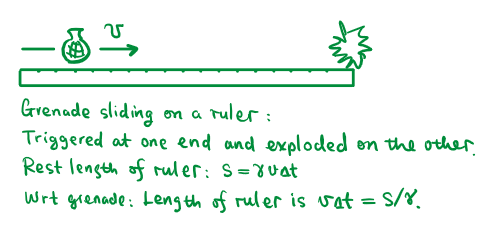
\includegraphics[width=0.35\textwidth]{grenade_length_contraction}}

	It still has lifetime $\Delta t$ (wrt itself). Though it would think that it has flown a distance $v \Delta t = s/\gamma$. But the observer standing on the ground thinks that it has flown a longer distance (wrt a static observer). How can it be?

	To make the situation clearer, let us put a ruler on the ground, and let the grenade slide over the ruler. The rest length of the ruler is $s = \gamma v \Delta t$.

	Wrt the grenade, the ruler (and ground) is moving with $v$ for time $\Delta t$. Thus the ruler has length $s/\gamma$ wrt the grenade. 

	\tcblower

	To conclude, a moving ruler is shorter by $1/\gamma$ if placed parallel to the motion direction. Also recall that if the ruler is perpendicular to the motion direction, then the length does not change.
}
	

We would have closed up the section here. But what happened during $\Delta t$ time in a grenade is opaque. Let us construct a light ruler to see what happens explicitly, which can also give insight on velocity addition. 

\textbox{(Optional) Length contraction from the light ruler (4-step reasoning)}{\index{length contraction from moving ruler}
	Although we have got the result, it is a good practice to derive it using another way. Let us construct a light ruler and study how it contracts. This will explicitly verify our promise: No matter how the ruler is defined, it should contract the same way. To see that, let us apply our familiar 4 steps:
	\tenum{
		\item In a static frame, the length of the ruler is $D = \frac{1}{2} c \Delta t$, where $\Delta t$ is the time interval between the emission and detection of light.

		\item Now we load the light ruler on Alice's car. The situation and the spacetime diagram that Bob finds are in the figures below. 

		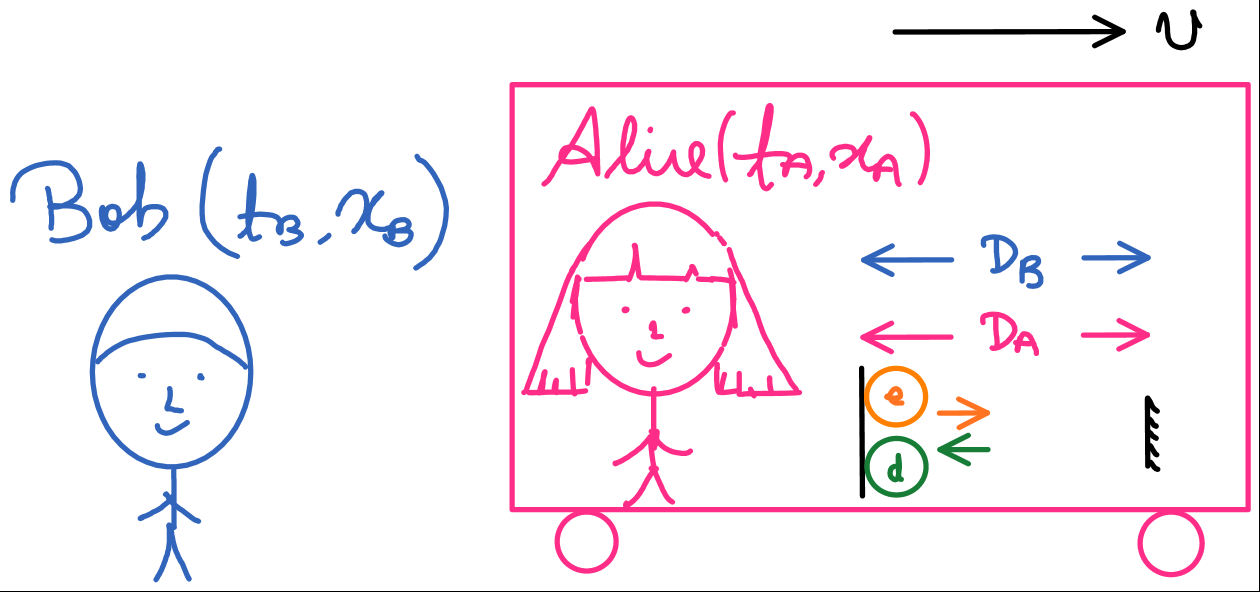
\includegraphics[width=0.5\textwidth, trim={0 3pt 3pt 0}, clip]{light_ruler}
		\hspace{0.1\textwidth}
		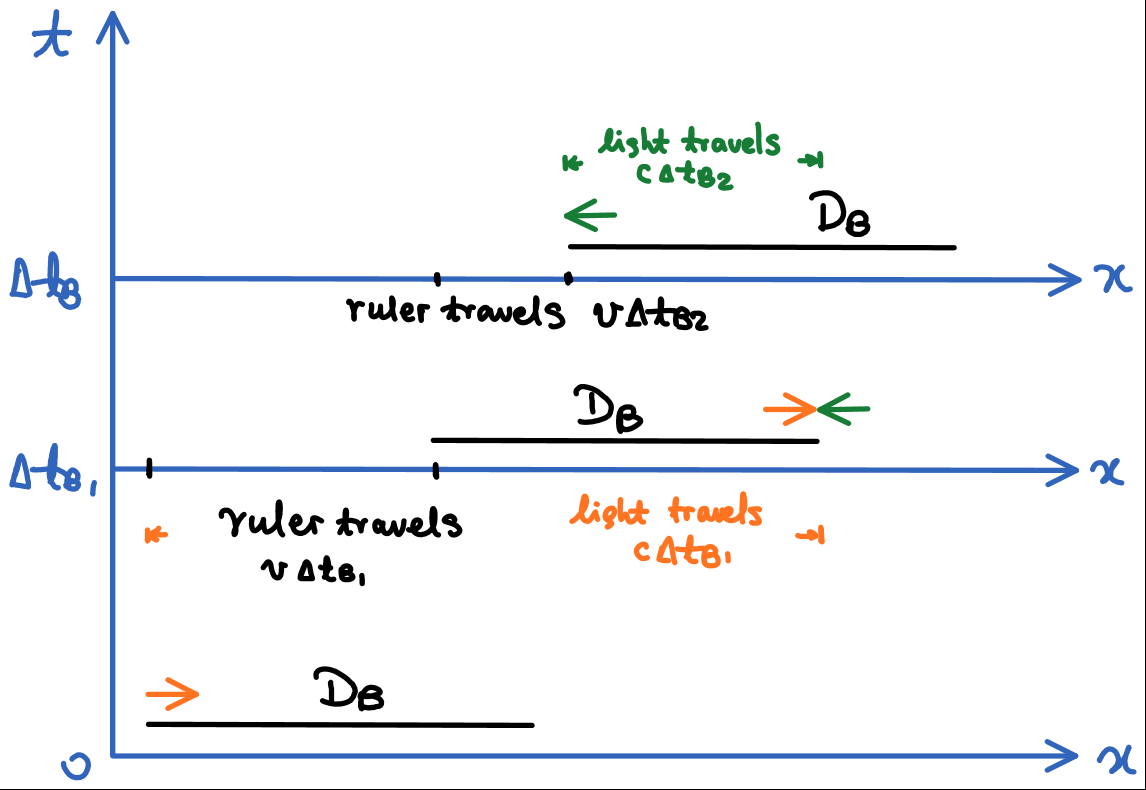
\includegraphics[width=0.6\textwidth, trim={0 2pt 2pt 0}, clip]{light_ruler_2}

		According to ($\mathbb{R}$), Alice consider the length of the ruler to be
		\begin{align}
		\label{eq:ruler_Alice}
		D_A = \frac{1}{2} c \Delta t_A~.
		\end{align}

		\item What length shall Bob get? We first divide the time interval $\Delta t_B$ into two parts: $\Delta t_{B1}$ and $\Delta t_{B2}$ for the time interval from the emitter to the mirror and from the mirror to the detector, respectively. From the above figure (right panel),
		\begin{align}
		\label{eq:bobx}
		c\Delta t_{B1} = D_B + v \Delta t_{B1}~, \qquad
		c\Delta t_{B2} = D_B - v \Delta t_{B2}~.
		\end{align}
		Thus
		\mtextbox{Meaning of $D_B$}{Be reminded that $D_B$ is NOT the length of Bob's ruler. But rather, it's the length of Alice's ruler (i.e. moving with Alice) in Bob's frame. So wrt Bob (static observer), Alice's ruler (moving ruler) contracts.}
		\begin{align}
		\label{eq:bobt}
		\Delta t_B \equiv \Delta t_{B1} + \Delta t_{B2} = \frac{D_B}{c-v} + \frac{D_B}{c+v} = \frac{2}{c} \frac{D_B}{1-\frac{v^2}{c^2} }
		= \frac{2}{c} \gamma^2 D_B~,
		\end{align}
		where as always, $\gamma\equiv \frac{1}{\sqrt{1-v^2/c^2}} $. Thus
		\begin{align}
		\label{eq:bobalice}
		D_B = \frac{c}{2} \frac{\Delta t_B}{\gamma^2} = \frac{c}{2} \frac{\gamma \Delta t_A}{\gamma^2} 
		= \frac{c}{2} \frac{\Delta t_A}{\gamma} = \frac{D_A}{\gamma}~.    
		\end{align}
		Again, we arrive at the conclusion that moving ruler contracts in the motion direction.

		\item For all rulers, one should get the same conclusion as the light ruler.
	}	
}

\mtextbox{(Optional) A speedmeter}{
	What's the motivation to replace $c$ with $v$ in one way? We can ask what this apparatus can do when it's at rest. From $\Delta t = D/u + D/c$, as we have defined $\Delta t$ and $D$, we can solve $u$. Thus, the apparatus is a speedmeter. No wonders that a speedmeter can tell you about speed addition.
}
\textbox{(Optional) A first look at velocity addition}{\index{velocity addition: first look}
	Let's slightly modify the light ruler: replace the light from emitter to mirror into a moving particle, with speed $u_A$ wrt Alice. After the ``mirror'' gets the particle, the ``mirror'' still sends back a beam of light (thus it shouldn't actually be called a mirror though). Then how the light ruler experiment get modified?
	\titem{
		\item Wrt Alice, for the particle forward, $u_A \Delta t_{A1} = D_A$; and for light moving back, $c \Delta t_{A2} = D_A$. Thus,
		\begin{align}\label{eq:fl-veladd1}
			\Delta t_A = \Delta t_{A1} + \Delta t_{A2} 
			= D_A \left( \frac{1}{u_A} + \frac{1}{c}  \right)~.
		\end{align}

		\item Wrt Bob, he will find the particle moving at a different velocity $u_B$. For the particle moving forward, $u_B \Delta t_{B1} = D_B + v \Delta t_{B1}$; and for light moving back, $c\Delta t_{B2} = D_B - v \Delta t_{B2}$. Thus,
		\mtextbox{(Optional) The additive rapidity}{Eq.~\eqref{eq:add-eg} looks ugly. Wouldn't nature be simpler? But who told us velocity is the best variable to describe motion? Let us define \emph{rapidity}:\label{rapidity} $\phi(v) \equiv \mathrm{arctanh} (v/c)$. Inserting this definition to Eq.~\eqref{eq:add-eg}, we simply get
		$$ \phi(u_B) = \phi(u_A) + \phi(v)~. $$
		Thus rapidity is the variable that is actually additive. 
		\tcblower
		Why hyperbolic functions arises here (they originally are functions to parameterize a hyperbolic curve $x^2-y^2=1$ with additive parameters, just as what trigonometric functions sin, cos, tan are functions to parameterize a circle $x^2+y^2=1$ with additive angles)? Do the hyperbolic functions imply a new underlying math structure? Why motion in such a formula looks not like division of space and time, but rather hyperbolic rotation of space and time? We will return to this question in section \ref{sec:geometry}.
		}
		\begin{align}\label{eq:fl-veladd2}
			\Delta t_B = \Delta t_{B1} + \Delta t_{B2}
			= D_B \left(  \frac{1}{u_B-v} + \frac{1}{c+v}  \right)~.
		\end{align}
		\item We already know that $\Delta t_B = \gamma \Delta t_A$ and $D_B = D_A/\gamma$. Now divide \eqref{eq:fl-veladd2} by \eqref{eq:fl-veladd1} (LHS and RHS, respectively), we get
		\begin{align} \label{eq:add-eg}
			u_B = \frac{u_A + v}{1+u_A v / c^2} ~. 
		\end{align}
	}
	When taking $u_A\rightarrow c$ limit, we find that $u_B\rightarrow c$, consistent with $(\mathbb{C})$. In section \ref{sec:lorentz}, you will learn a more general version of the velocity addition formula.
}

% \textbox{(Optional) Length contraction from two moving rods}{
% 	Alice and Bob carry rods and moves with relative speed $v$ towards each other. A light signal is emitted from the left end of the rods when the left ends coincide. The light signal reaches the right end of the rods when the right ends coincide.

% 	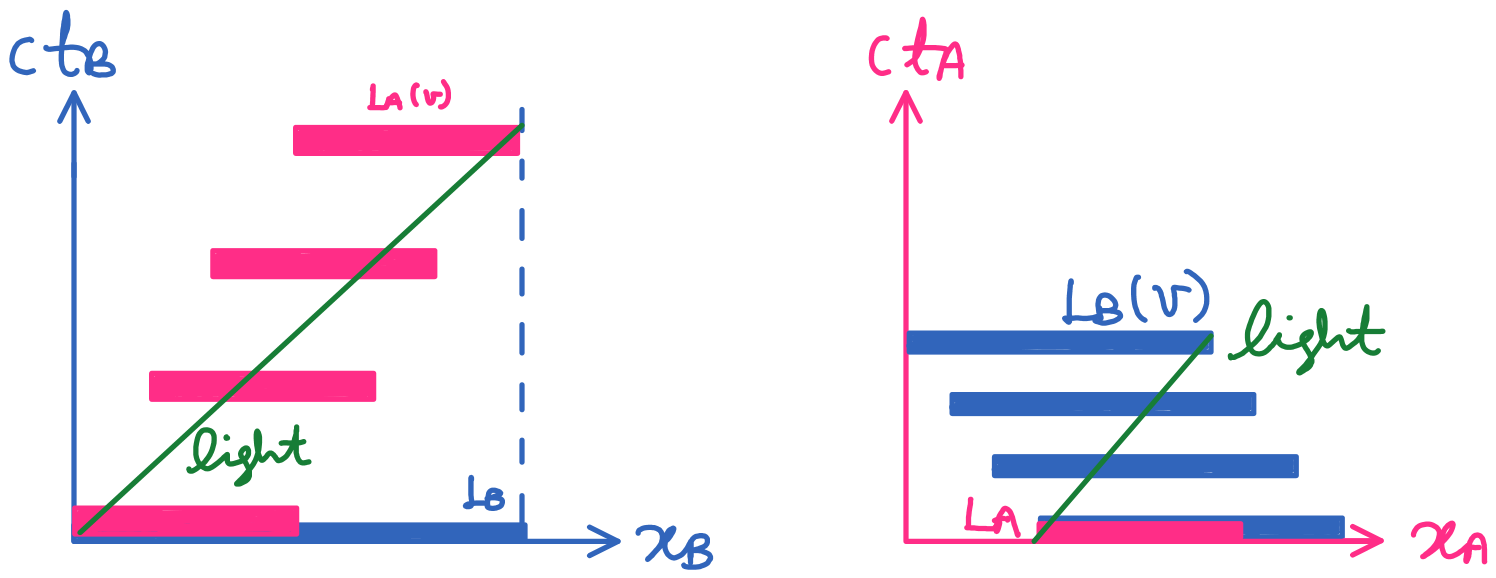
\includegraphics[width=\textwidth]{contraction3}

% 	For the situation of the above figure, According to Bob (left panel of the figure):
% 	\begin{align}
% 	\label{eq:c3bob}
% 	\frac{L_B-L_A(v)}{v} = \frac{L_B}{c}~,  \quad\rightarrow\quad
% 	\frac{L_A(v)}{L_B} = 1- \frac{v}{c} ~,  
% 	\end{align} 
% 	and according to Alice (right panel of the figure),
% 	\begin{align}
% 	\label{eq:c3alice}
% 	\frac{L_B(v)-L_A}{v} = \frac{L_A}{c}~,  \quad\rightarrow\quad
% 	\frac{L_B(v)}{L_A} = 1+ \frac{v}{c} ~.
% 	\end{align}
% 	Multiply the above two equations, 
% 	\begin{align}
% 	\label{eq:c3m}
% 	\frac{L_A(v)}{L_A} \frac{L_B(v)}{L_B} = 1- \frac{v^2}{c^2}~.   
% 	\end{align}
% 	This relation holds for all lengths \marginnote{Change $L_A$, the RHS does not change, so the RHS should not depend on $L_A$. For the same reason, the RHS does not depend on $L_B$}. As a result, we must have
% 	\begin{align}
% 	\label{eq:c3}
% 	\frac{L_A(v)}{L_A} = \frac{L_B(v)}{L_B} = \sqrt{1- \frac{v^2}{c^2}} = 1/\gamma~.
% 	\end{align}
% }

We have got two results from the light clock now: time dilation; and after time dilation have become known, we rotate the light clock to get length contraction. Now that length contraction have become known, can we get something else?

\section{Meaning of the ``Same Time'' (Simultaneity)} \label{sec:same-time}

Moving ruler contracts. Now, is there a twin ruler paradox? If Alice and Bob each holds a ruler along their motion direction, and when they meet, they compare the length of their ruler, can they find each other's ruler shorter? How can that happen?

The key observation is that, to be fair, they have to compare the two ends of the ruler at the same time. Wait, do they have the same concept of the same time?

\subsection{Simultaneity Depends on Which Observer}

\needspace{0.1\textwidth}
\mtextbox{Why introducing two objects?}{Actual objects $P$, $Q$ are needed to find an observer standing at the midpoint. Because a midpoint is defined for two points in space ($P$ and $Q$), not for two events ($E_P$ and $E_Q$) in spacetime.}
\textbox{The meaning of simultaneity wrt an observer}{\index{simultaneity}\index{same time}
	Consider two small objects $P$ and $Q$, not moving wrt each other.
	An observer is standing exactly at the midpoint of $PQ$, and not moving wrt $PQ$. This can be practically done with a static ruler: Let $P$ be at the 0m point, $Q$ be at the 1m point, and the observer at the 0.5m point.

	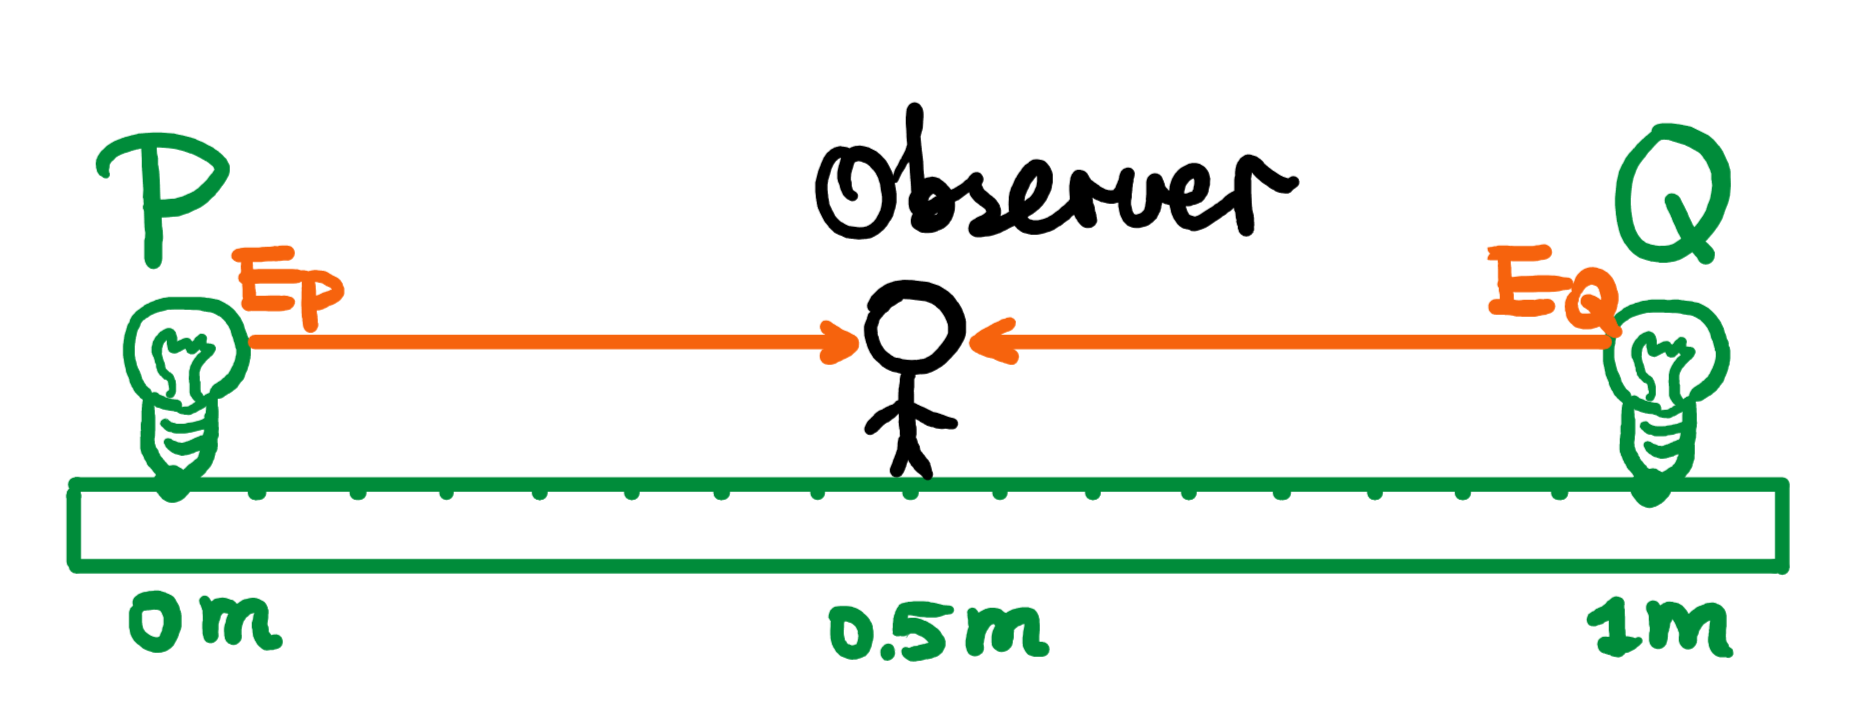
\includegraphics[width=0.4\textwidth]{st_ground}
	\mtextbox{Relating to the time of a frame}{Previously, we have introduced the time of a reference frame -- at different positions, time are synchronized using light signals, deducting the time used for light propagation. Here, the concept of simultaneity means that $E_P$ and $E_Q$ happens at the same coordinate time in this static frame.}

	Introduce two events: event $E_P$ happens to object $P$; and event $E_Q$ happens to object $Q$. For example, $E_P$ and $E_Q$ are the turn-on time of light bulbs at $P$ and $Q$, respectively. Recall that each event happens at a particular moment.

	Now we are ready to define whether $E_P$ and $E_Q$ happens at the same time, or one is earlier/later than the other, wrt the observer:
	
	If the light signal from $E_P$ and $E_Q$ reach the observer at the same time, then $E_P$ and $E_Q$ happens at the same time. Otherwise, whichever reaches the observer earlier happens earlier.
}

\mtextbox{Am I wasting your time?}{
	Oh, it looks that I am wasting your time by explaining something you already know since kindergarten. This is true. However, one little step further will need university education -- load the device into a car.
	\tcblower
	Einstein said with great modesty: 
	``How it happened that I in particular discovered the relativity theory, it seemed to lie in the following circumstance. The normal adult never bothers his head about space-time problems. Everything there is to be thought about it, in his opinion, has already been done in early childhood. I, on the contrary, developed so slowly that I only began to wonder about space and time when I was already grown up. In consequence I probed deeper into the problem than an ordinary child would have done.'' 
}
\textbox {A spacetime diagram of the above scenario}{
	Let us draw the events in a ``spacetime diagram''. Spacetime diagrams will turn out to be useful tools in studying relativity. On a spacetime diagram:

	\begin{minipage}
		{0.58\textwidth}
		\titem{
			\item An event is a point.
			\item Light travel $45^\circ$ lines.
			\item An object (or observer, except light) is a line (called world line) with $|$slope$| > 45^\circ$ everywhere.
			\item An inertial observer is a straight line.
			\item A static object is a line parallel to the $ct$ axis.
			\item Events at the same time are parallel to the $x$ axis.
		}
	\end{minipage}
	\hspace{0.02\textwidth}
	\begin{minipage}
		{0.4\textwidth}
		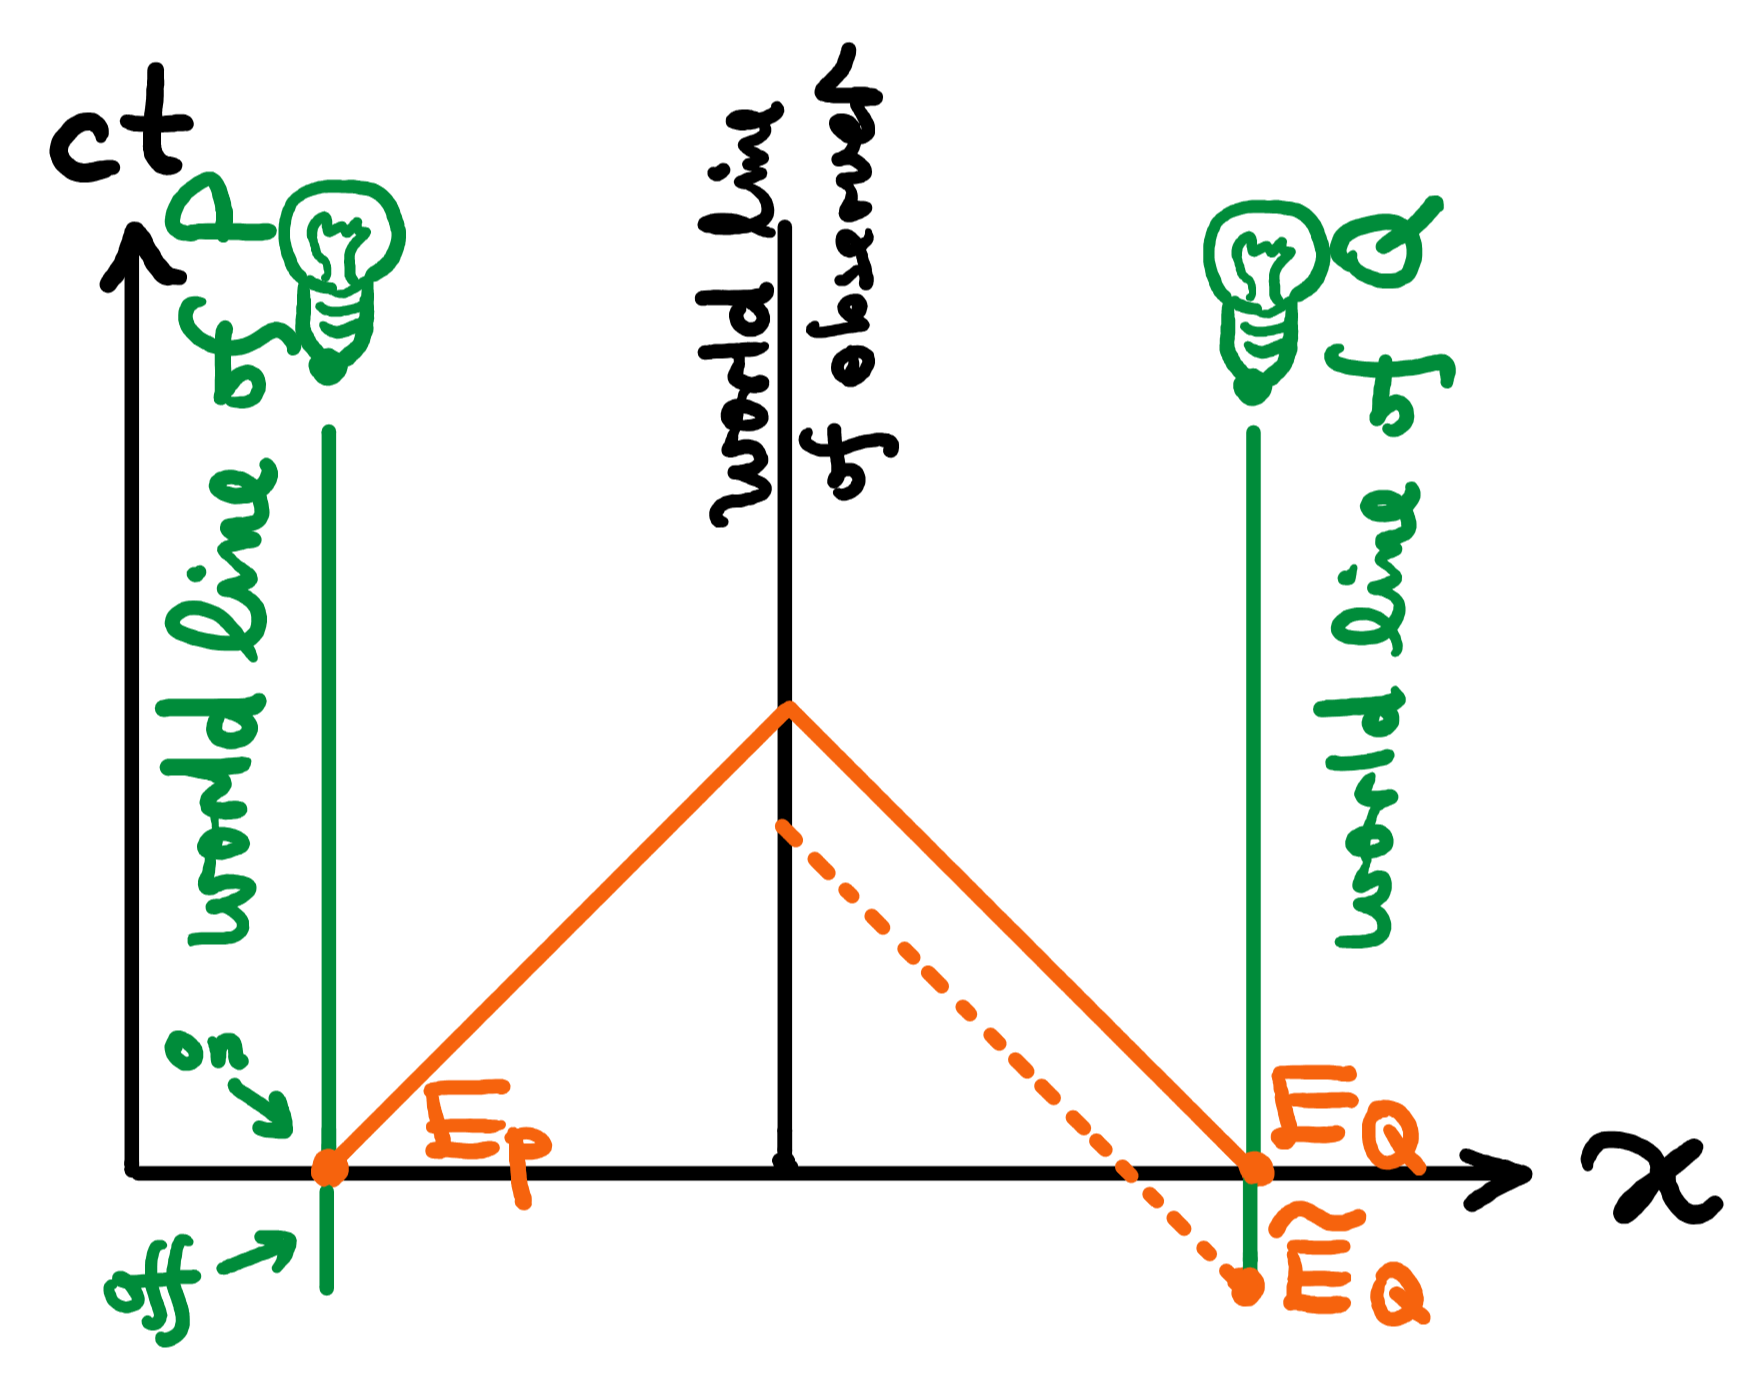
\includegraphics[width=\textwidth]{st_diag_ground}
	\end{minipage}

	If the light rays connecting $E_P$ and $E_Q$ reaches the world line of the observer at the same point, they happen at the same time wrt the observer. On the contrary, $\widetilde{E}_Q$ is considered earlier than $E_P$ wrt the observer as the light ray from $\widetilde{E}_Q$ arrives earlier at the observer.
}

\textbox{Simultaneity is a relative concept (4-step reasoning)}{\index{simultaneity is relative}
	\tenum{
		\item We have defined simultaneity for a static observer with the above $P$-observer-$Q$ system.
		\item Let us load the system into a car and let the moving observer be Alice. Let us study the events $E_P$ and $E_Q$, which happen at the same time wrt Alice. In our example, that corresponds to the light bulbs turning on at the same time at $P$ and $Q$ wrt Alice. See left panel of the below figure.

		\begin{minipage}
			{0.55\textwidth}
			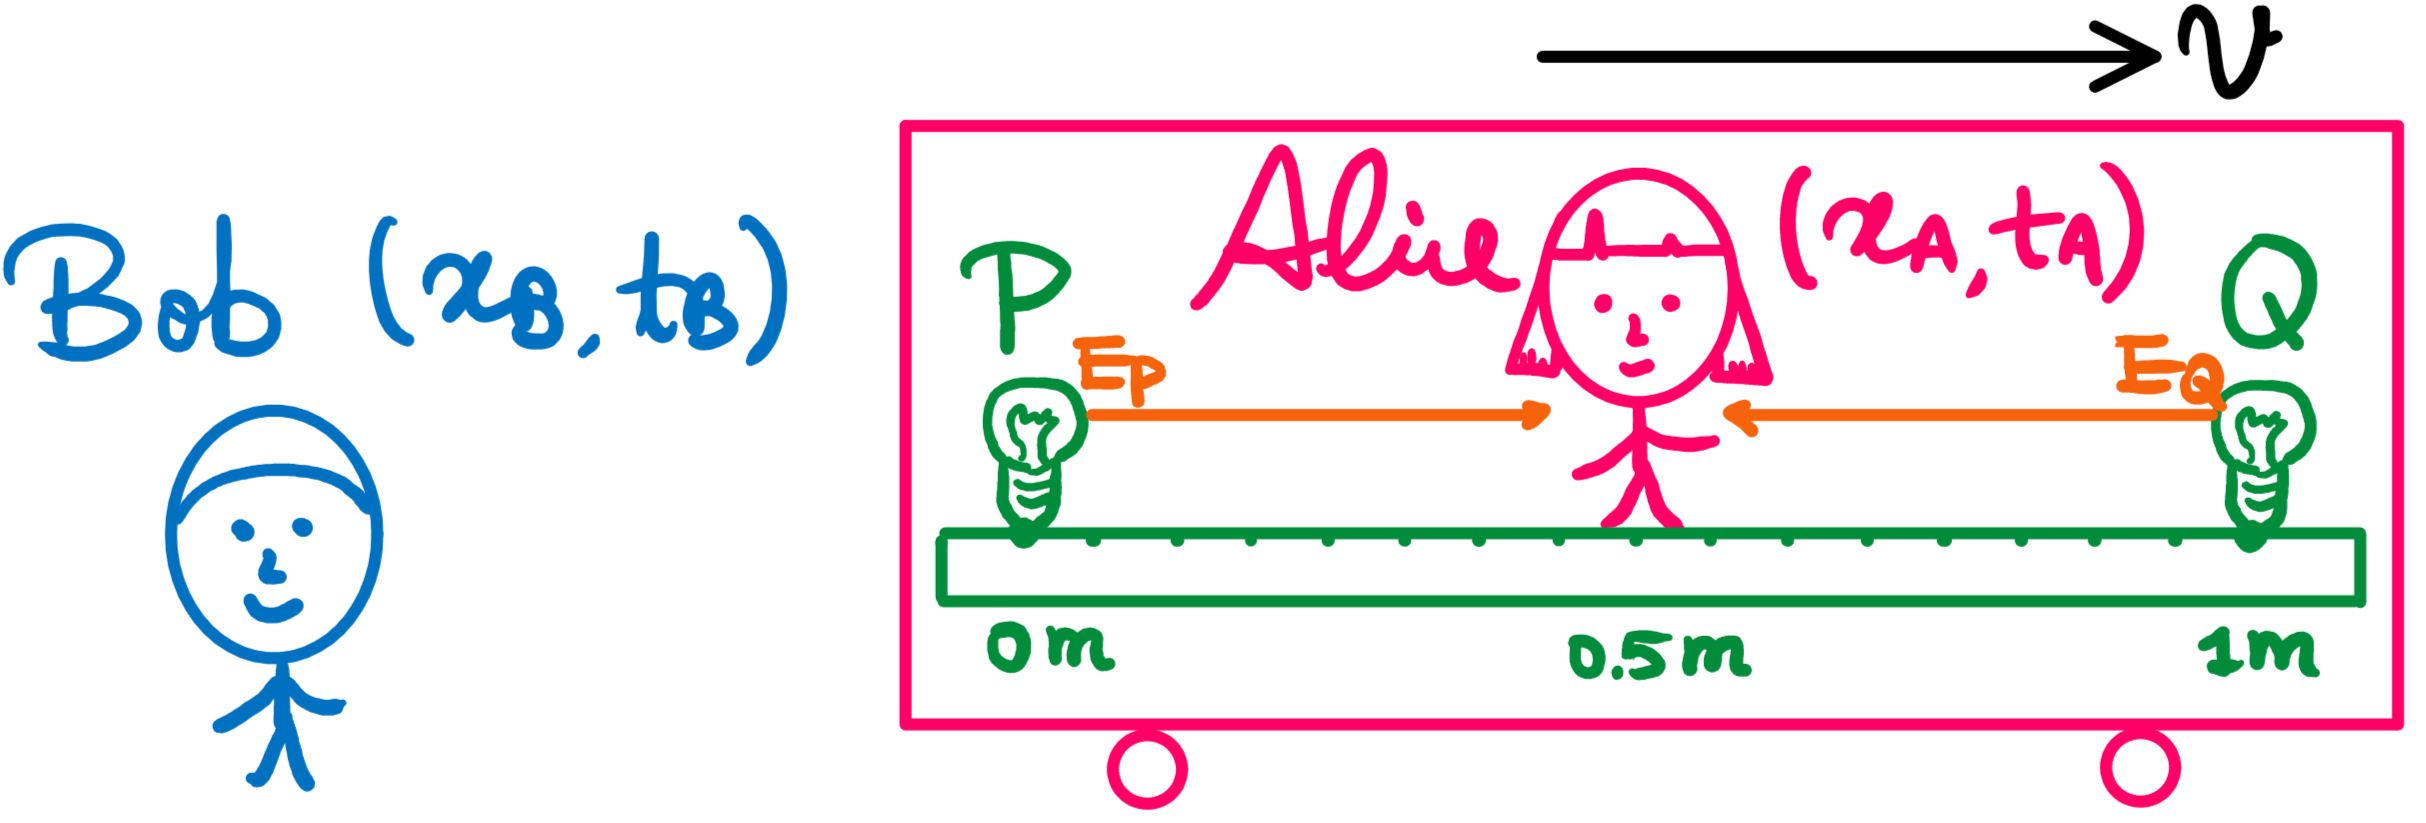
\includegraphics[width=\textwidth]{st_car}
		\end{minipage}\hspace{0.1\textwidth}
		\begin{minipage}
			{0.35\textwidth}
			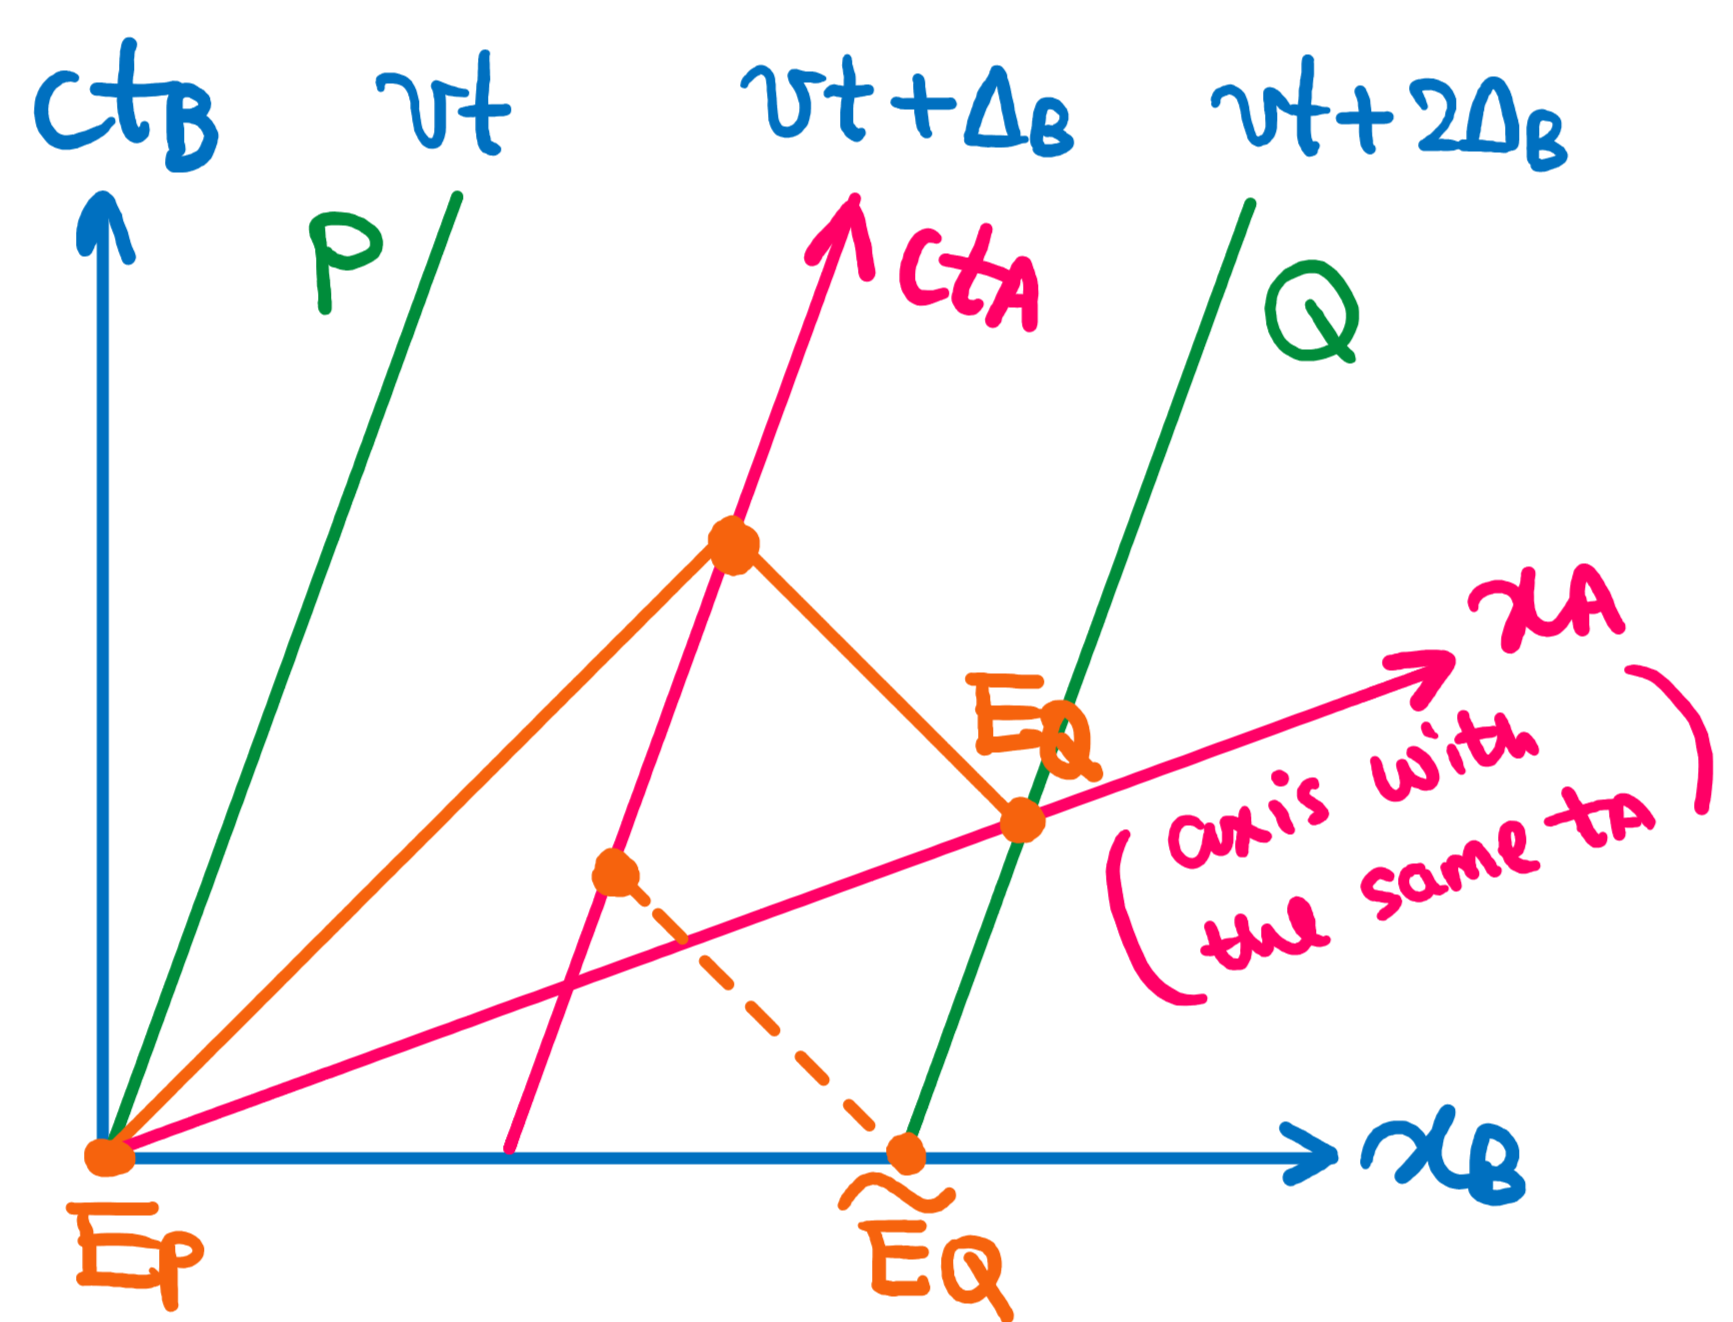
\includegraphics[width=\textwidth]{st_diag_car}
		\end{minipage}

		\mtextbox{Bob's spacetime diagram}{
			\mtitem{
				\item Draw Bob's axes and world lines $A$, $P$, $Q$.
				\item Draw the event that two beams of light meet Alice.
				\item Draw the history of these two beams of light as $45^\circ$ lines.
				\item The intersection of light and $P$, $Q$ are events $E_P$, $E_Q$.
				\item Compare the time of $E_P$ and $E_Q$ in Bob's frame.
				\item Draw the spacetime axes of Alice's frame in Bob's frame.
			}
		}
		\item Wrt Bob, do $E_P$ and $E_Q$ happen at the same time? In other words, do $E_P$ and $E_Q$ have the same time coordinates in Bob's frame? Making use of a spacetime diagram in Bob's frame (right panel of the above figure), we immediately find that $E_P$ is earlier than $E_Q$ wrt Bob. On the contrary, an event $\widetilde{E}_Q$ considered to be at the same time with $E_P$ wrt Bob, is considered earlier than $E_P$ wrt Alice.
		
		\item The relativity of simultaneity is not only true for the $P$-observer-$Q$ system, but for all consistent definitions of simultaneity ($\mathbb{R}$).
	}
}
Now you should be able to resolve the puzzle of ``who wrote the letter first''.

\textbox{Recap: equal time slices}{
	\begin{minipage}
		{0.55\textwidth}
		To condense the above analysis into one figure: When Alice is moving wrt Bob, the coordinate system of Alice drawn in Bob's coordinate system is as the figure to the right. It is similar to rotation, but both space and time axes oddly fold inwards. We will discuss this transformation (Lorentz transformation) in more details later. You should pay special attention on the equal time lines wrt Alice on this figure -- different from that wrt Bob.
	\end{minipage}
	\hspace{0.1\textwidth}
	\begin{minipage}
		{0.35\textwidth}
		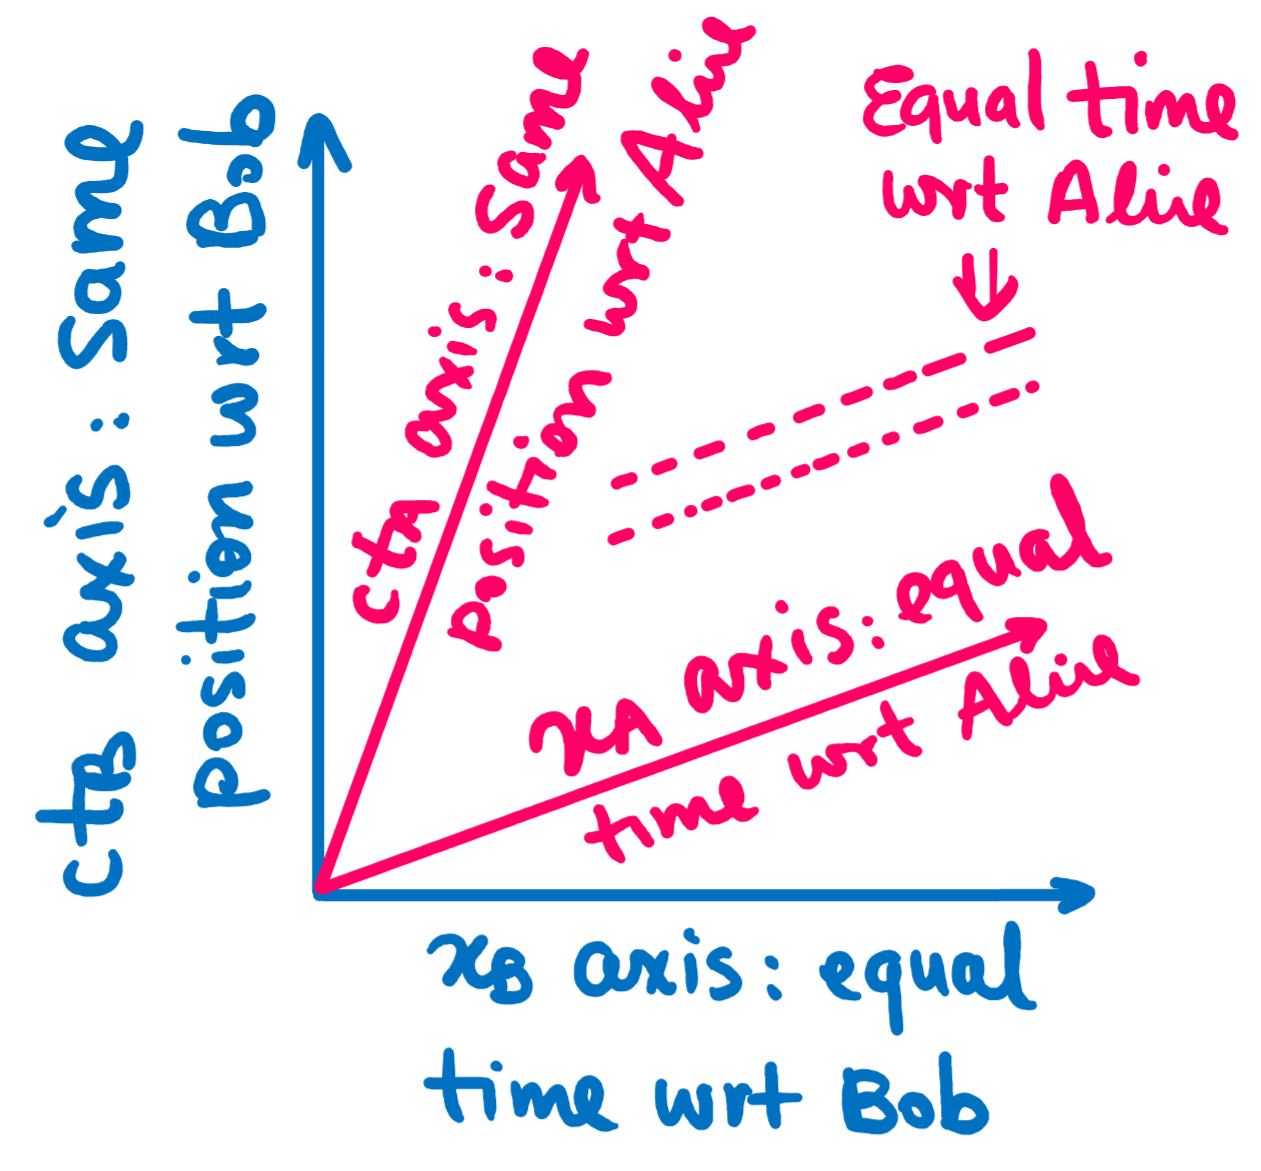
\includegraphics[width=\textwidth]{equal_time_simplified}
	\end{minipage}
}

\mtextbox{Can SR describe acceleration?}{There is a common misconception saying ``special relativity cannot describe the experience of an accelerating observer''. This is \emph{wrong}. The laws of special relativity (time dilation, length contraction, and more later) are expressed in inertial frames (just because the laws are mathematically simpler in inertial frames). Thus, we need to \emph{use an inertial frame} to apply these laws to our question. However, we can \emph{calculate in this inertial frame} what an accelerating observer sees (how light reach her eyes, for example). In this way, the experience of an accelerating observer is described \emph{with the help of an auxiliary inertial frame}.}
\textbox{Twin paradox revisited}{\index{twin paradox: revisited}
	\begin{minipage}
		{0.6\textwidth}
		In our twin paradox, Alice is not in an inertial observer at the turn around time. Thus she cannot use special relativity of an inertial observer to \emph{directly} explain her experience. However, Bob can help her to figure out what happens at the turn-around:

		Before and after the turn-around, Alice is in two \emph{different} inertial frames. Bob's age ``jumps'' when Alice switches from the before-turn-around frame to the after-turn-around frame. Thus in Alice's frames, there is a sudden change in Bob's age.

		As mentioned, to describe what Alice sees (light arrives in her eyes), light propagation time needs to be added. I will leave the details for your exercise.
	\end{minipage}
	\hspace{0.01\textwidth}
	\begin{minipage}
		{0.3\textwidth}
		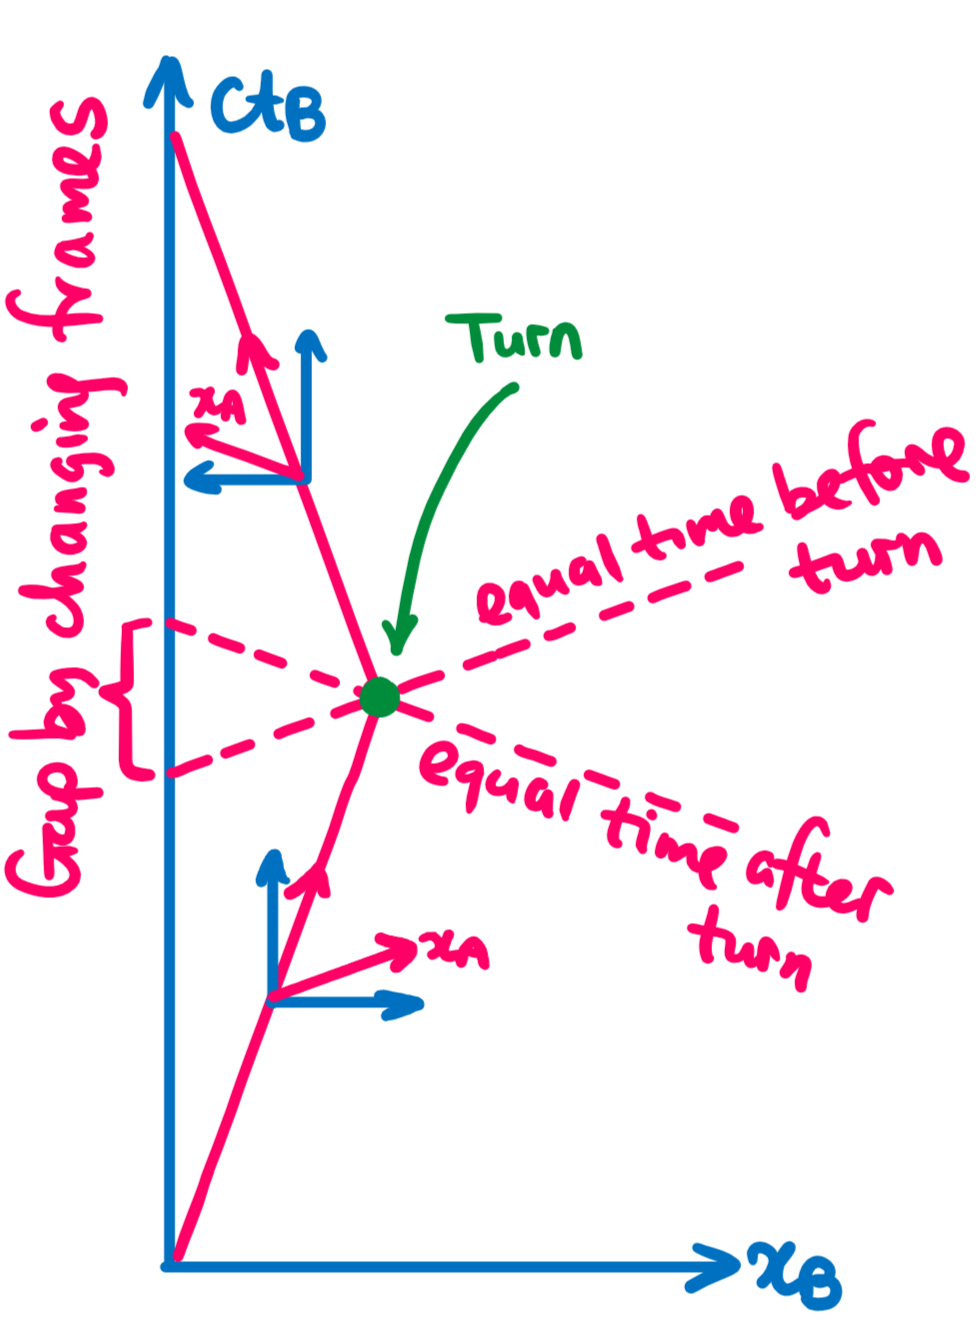
\includegraphics[width=\textwidth]{same_time_twin}
	\end{minipage}
}

\subsection{Causality and Types of Separations}

Now we have understood: the concept of simultaneity is relative to observers. For example, Alice and Bob may consider differently on who wrote the letter first. In other words, time orders of some events (here two events: Alice writes her letter; Bob writes his letter) are reversible. 

A natural question then is: Are all time orders between events reversible?

\textbox{Time order associated with cause and effect}{\index{causality}
	Consider an example: Lightning strikes on a tree, and then the tree dies. There are two events here:
	\marginnote{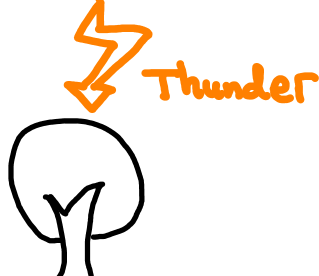
\includegraphics[width=0.15\textwidth]{thunder}}
	\tenum{
		\item Event E(strike): Lightning strikes on the tree.
		\item Event E(die): The tree dies. This is an \emph{effect}, \emph{caused} by E(strike).
	}
	May a moving observer Ms.~Bright observe that E(die) happens earlier than E(strike)?

	\mtextbox{Correlation}{Cause-effect is a special case of correlation (conditional probability). If events E1 and E2 have nontrivial correlation, maybe
	\mtitem{
		\item E1 causes E2
		\item E2 causes E1
		\item Both E1 and E2 are caused by something else
	}}
	\tcblower
	The cause-effect relation (known as causality) is at the heart of physics. Physics is about prediction of how an initial state evolves with time. In other words, the cause-effect relation is how questions get explained in physics -- ``Why (effect)? Because (cause).'' 
}

As causality is so important, we hope that it is preserved in special relativity. Happily, special relativity is indeed \emph{consistent} with causality. Having that said, causality is an independent postulate added to special relativity. In other words, special relativity itself does not \emph{derive} causality. Let us now see how causality and relativity work together.

\mtextbox{No superluminal lightning either}{
	For causal order to be respected, not only Ms. Bright is not supposed to travel faster-than-light; but also no lightning (or any information causing the death of the tree) can be superluminal either. Otherwise causality is violated even with subluminal Ms. Bright.
}
\textbox{Special relativity without superluminal motion is consistent with causality}{\index{causality and relativity}
	\begin{minipage}
		{0.5\textwidth}
		Spacetime diagram of subluminal Ms. Bright and superluminal Ms.~Bright. For any subluminal observer, the world line of the tree has slope greater than $45^\circ$. Then, as long as Ms.~Bright moves no faster than the speed of light, she cannot flip the order of E(strike) and E(die).
	\end{minipage}
	\hspace{0.05\textwidth}
	\begin{minipage}
		{0.4\textwidth}
		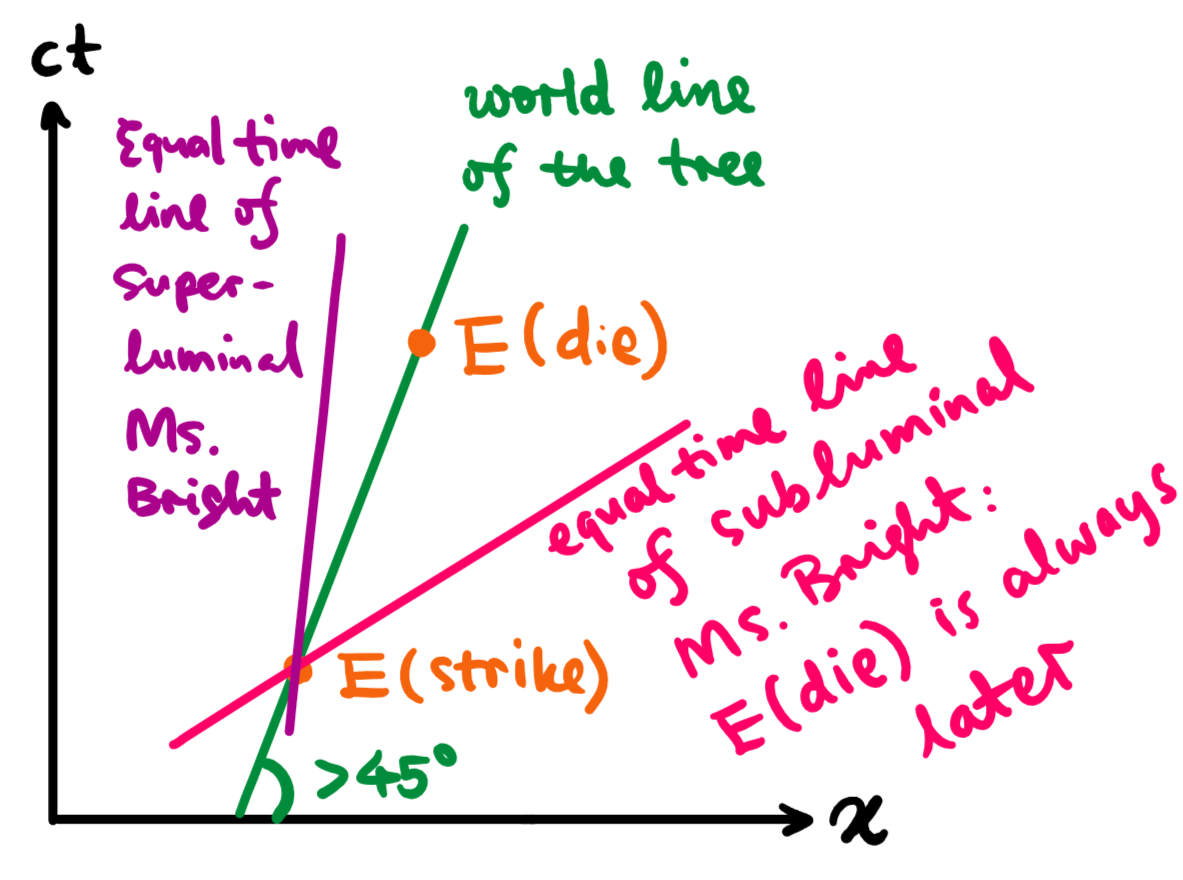
\includegraphics[width=\textwidth]{sr_consistent_causality}
	\end{minipage}

	\mtextbox{Buller's poem (1923)}{
	There was a young lady named Bright;\newline
	Whose speed was far faster than light;\newline
	She set out one day;
	In a relative way;\newline
	And returned on the previous night.	\mnewline
	We hope this to be forbidden. Otherwise, what if Ms.~Bright returned to the previous night, and locked herself in the room, how can her superluminal trip happen at all? \mnewline
	So far, the most convincing explanation is that, superluminal trip should be forbidden. Having that said, the possibility of a time machine is an open question for modern physics.
	}
	\tcblower

	Thus, if superluminal movers are forbidden, then the cause-effect order is preserved. In this course, we will assume that superluminal motion is indeed forbidden in special relativity. This is consistent with all known experiments.

	More generally, no information can be sent faster than the speed of light. Because information must be sent by matter after all. And from the consistency of the theory, information can bring causal connection between events. Thus if information can be sent faster than light, then the same problems of superluminal motion can arise. 

	You may have an excellent question at this point: What if we push Ms.~Bright so she accelerates from subluminal to superluminal? It is in fact impossible. We will come back to this point later.

	In general relativity, you may hear that things can go superluminal, for example, for cosmic expansion. This is right or wrong. One has to first define velocity precisely. We will come back this point at the end of this course, in the cosmology section.
}


\textbox{Causal structure of spacetime: past and future light cones\index{light cone}}{
	From separation of events, given a spacetime point (say, you at the present time), the spacetime is divided into three different regions according to the causal connection to the 
	\marginnote{\cg{0.3}{lightcones}}
	observer.

	\titem{
		\item Past light cone. This region contains all the causes of you up to now. You have not yet seen anything beyond this region.
		\item Future light cone. This region contains all the effects by you from now on. You can no longer change anything beyond this region.
		\item Outside both past and future light cones: there is no cause-effect relations between the present version of you and any point there. 
	}
}
\textbox{No perfectly rigid body in relativity}{\index{rigid body (non-existing)}
	Let's consider a thought experiment: Alice and Bob are separated by 5 light years. And they hold a 5-light-year-long rod, which is a perfect rigid body. Then can Alice and Bob send information faster than light by pushing the rod?

	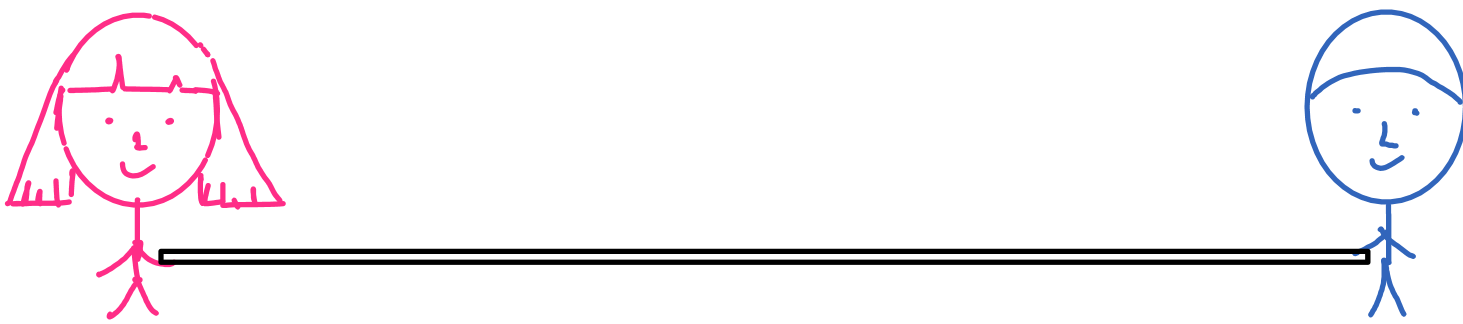
\includegraphics[width=0.8\textwidth]{ABrod}

	\tcblower

	The answer is a simple straight no. Because no information can be faster than light, perfectly rigid body does not exist in special relativity. 

	If this answer is too brute, we can also see dynamically what happens. The rod is (usually) made of atoms and the force propagating between atoms need at least speed of light to react a push. 
}

The speed of light limit classifies the intervals between two events into 3 classes.

\textbox{Space-like, null and time-like intervals}{\index{space-like}\index{time-like}\index{null}
	There
	\marginnote{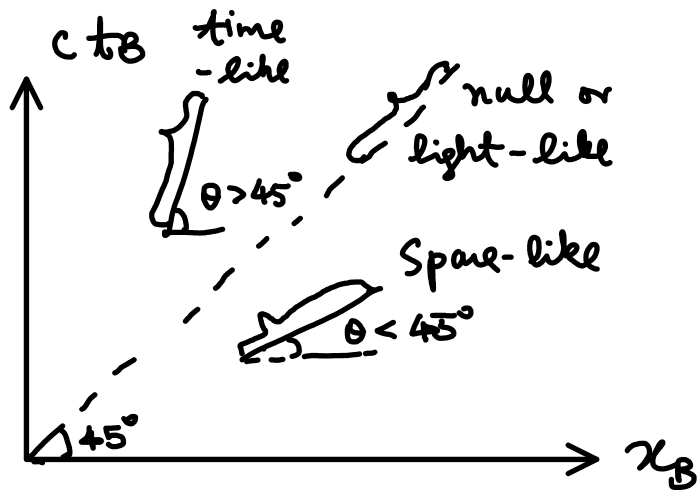
\includegraphics[width=0.35\textwidth]{space_time_null_like}}
	are three types of intervals between events.
	\titem{
		\item Space-like: with slope $<45^\circ$. There exists observer wrt whom two space-like separated events happen at the same time. The events are thus pure space separated wrt this observer. The time order of the events can be flipped for different observers.
		\item Time-like: with slope $>45^\circ$. There exists observer wrt whom two time-like events happen at the same position. The events are thus separated only in time wrt this observer. The time order of the events is absolute and has to be agreed on for all observers.
		\item Light-like (or called null): the boundary separating space-like and time-like intervals, with slope $45^\circ$. Light travels with light-like lines.
	}
}

\section{Example: The Ladder Paradox}\label{sec:ladder}

Let's apply what we have learned to get confused (or hopefully not).

\textbox{The ladder and the garage}{\index{ladder paradox: open garage}
	Consider a 15m long ladder (the ends are labeled P and Q). Alice holds it and moves it towards a garage, with speed 0.87c, i.e. $\gamma=2$. The garage is 10m long, and the front door and back door are labeled F and B, respectively. Bob sits static with the garage. 

	\cg{0.7}{ladder}

	\marginnote{\hfill 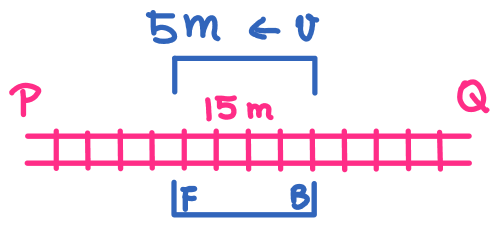
\includegraphics[width=0.25\textwidth]{ladderA}\hspace{0.02\textwidth}}
	
	What does Alice find? Alice finds that the garage moves, and thus the length of the garage is $10\mathrm{m}/2=5\mathrm{m}$. Thus the ladder does not fit in the garage. 

	What does Bob find? Bob finds that the ladder moves, and thus the length of the ladder is $15\mathrm{m}/2=7.5\mathrm{m}$. Thus the ladder fits in the garage.

	\marginnote{\hfill 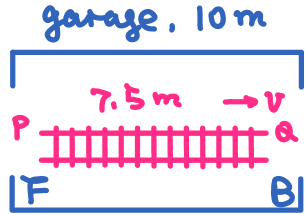
\includegraphics[width=0.2\textwidth]{ladderB}\hspace{0.02\textwidth}}

	Who is right?

	\tcblower

	\twocol{0.5}{0.01}{0.75}{
		Both are right. 
		
		Note that ``ladder fit in garage'' is not an event which localized at a spacetime point. Especially, there are two important events:

		\tenum{
			\item P enters front door F.
			\item Q exits back door B.
		}

		If \enumlabel{1} is earlier than \enumlabel{2}, then the ladder fits in the garage. If \enumlabel{2} is earlier than \enumlabel{1}, then the ladder does not fit in the garage.

		Wrt Alice, \enumlabel{2} is earlier than \enumlabel{1} (does not fit); Wrt Bob, \enumlabel{1} is earlier than \enumlabel{2} (fits). 
	}{
		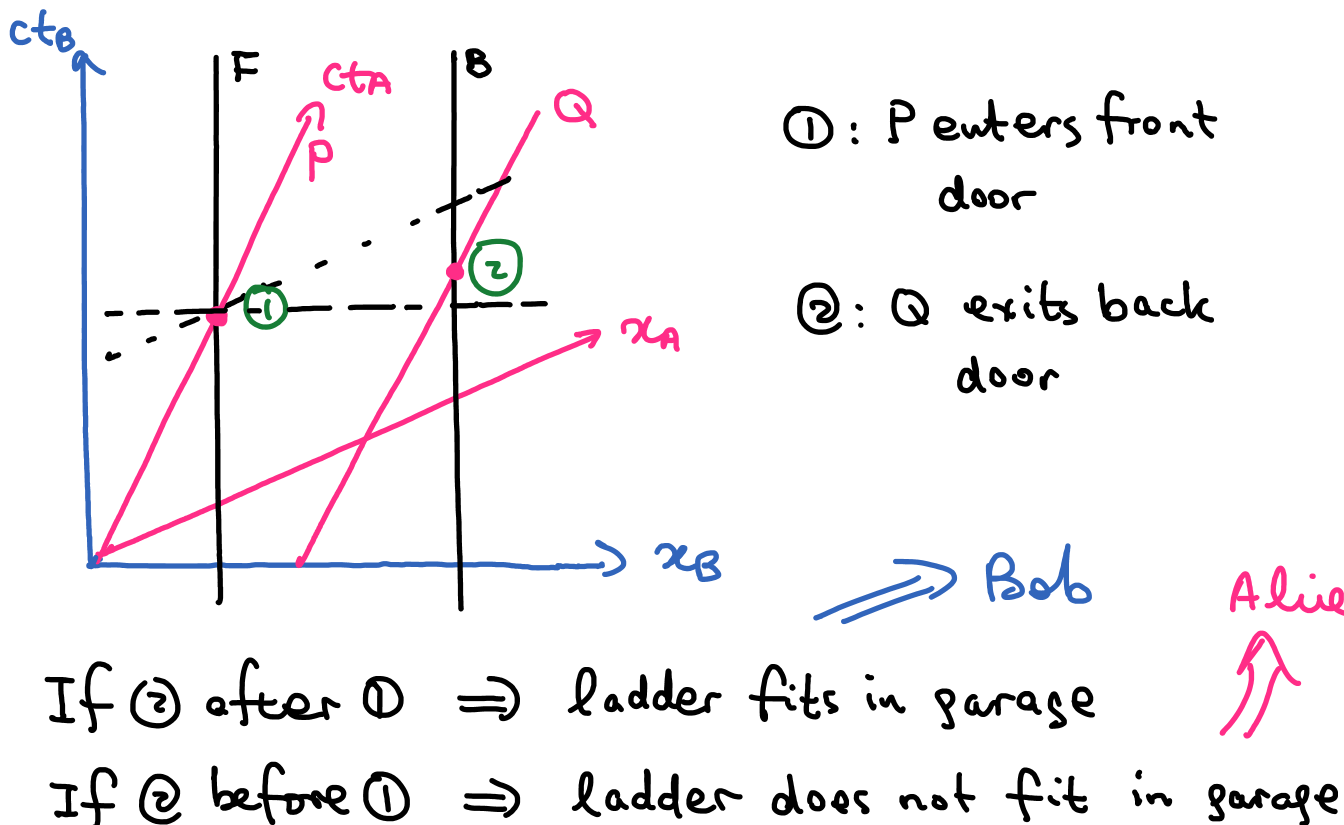
\includegraphics[width=\textwidth]{garage_st}
	}
}

\textbox{The ladder and the garage with doors}{\index{ladder paradox: closed garage}
\marginnote{Here we assume that Alice is still in an internal frame, no matter any part of the ladder may stop or not. }
Let's add a local event to sharpen what happens. Let the back door of the garage always be closed. Bob closes the front door once he finds the ladder moves in the garage.

	\cg{0.7}{garage_door}

	Now even Alice has to agree that the ladder is completely in the garage because the doors are closed. So the ``paradox'' becomes sharper: Alice thinks that the ladder is longer than the garage; but it is now completely in the garage!

	Resolution: Remember that in relativity, there is no perfectly rigid body. 

	Assuming that the door is relatively stronger and does not break, then the ladder must fall into parts. Wrt Alice: when Q stopped moving, the ``stop'' information has to be passed to P and it takes at least time $15\mathrm{m}/c$. During this time, the front door moved about $13$m. Thus $P$ is well inside $F$ by this time. Of course, it fits into the $5$m garage very well.

	On the other hand, if the ladder is relatively stronger and does not break, then the back door is broken and there is no difference from no back door.
}

\textbox{Replacing the garage by a trap}{\index{ladder paradox: trap}
	Let us further replace the binary doors by boundary of a trap.
	
	\cg{0.7}{trap}

	Bob' considers that Alice with the ladder start to fall in when the ladder is entirely in the trap. Thus Alice falls in. However, Alice considers herself still not yet fall-in before the Q point escapes. Who's right?
	\tcblower
	This really depends on how Alice holds the ladder. If Alice holds the ladder perfectly parallel to the ground and sliding on the ground, then Alice falls in. Because there is no perfect body. When $Q$ falls into the trap, $Q$ inevitably falls downwards. However, if Alice holds the ladder in the way a bit upwards, such that Q does not need ground support from the beginning, then Alice can escape.
}

\textbox{Replacing the garage by a circuit}{\index{ladder paradox: circuit}
	Let us stop destroying things and go electronic. Consider the situation below.

	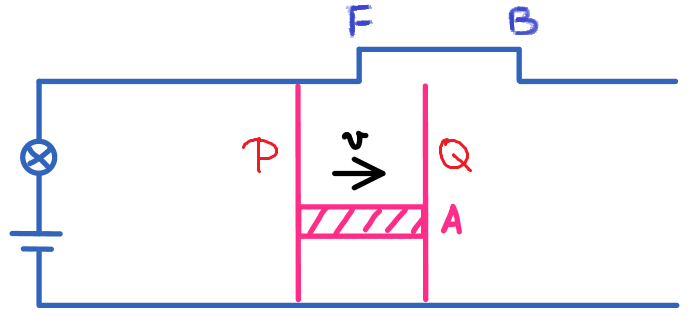
\includegraphics[width=0.6\textwidth]{light_paradox}

	Alice holds two moving conducting wires (they are isolated wrt each other). Both can close the circuit. Wrt Bob, there exists a time when neither of Alice's wires closes the circuit so the bulb shuts off for a moment. Wrt Alice, at least one wire touches the circuit all the time. So shall the bulb shut off?
	\tcblower
	The key to resolve the problem is that, electricity needs time to conduct. The speed of electricity is comparable to $c$, but still less than $c$. Thus wrt Alice, to keep the bulb on without a off-time gap, the electric current has to reach F before Q passes F. So there is an off-time wrt Alice, too.
}


\section{The Lorentz Transformation} \label{sec:lorentz}

\textbox{Alice and Bob need a rule for their coordinate transformations}{

	\twocol{0.55}{0.1}{0.3}{
		An event $P$ happened. Both the moving Alice and the standing Bob agree on the existence of the event. However, the same event has different coordinates in Alice's and Bob's frames.

		Given the coordinate of P: $(t_B, x_B)$ in Bob's frame, how to get the coordinate $(t_A, x_A)$ for the same event in Alice's frame?
	}{
		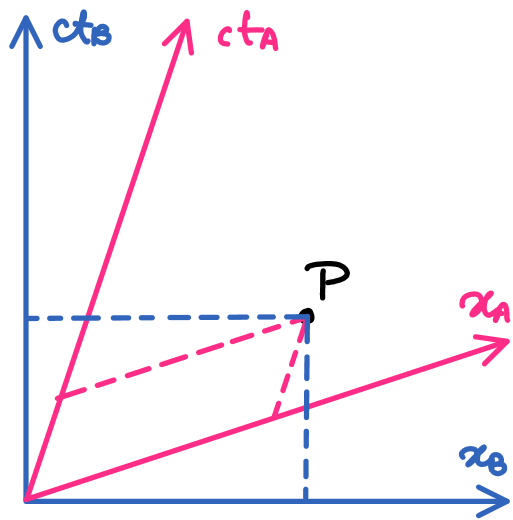
\includegraphics[width=\textwidth]{st_trans}
	}

	Recall that the transformation between inertial frames is called a boost. Thus the question can also be asked as: how does coordinates transform under a boost?

	\tcblower

	Before solving this problem, let us draw similarity between boost and rotation. 

	\twocol{0.5}{0.05}{0.45}{
		The case of rotation: Alice and Bob are not moving wrt each other, but facing different directions. Given Bob's coordinate of an object $(x_B, y_B)$, how to get Alice's coordinate for the same object $(x_A, y_A)$? Following relations of Euclidean geometry, we get: \index{rotation}
		\begin{equation}
			\label{eq:ss-rotation}
			\left\{
			\begin{aligned}
				x_A & = x_B \cos\theta + y_B \sin\theta \\
				y_A & = -x_B \sin\theta + y_B \cos\theta
			\end{aligned}
			\right.
		  \end{equation}
	}{
		  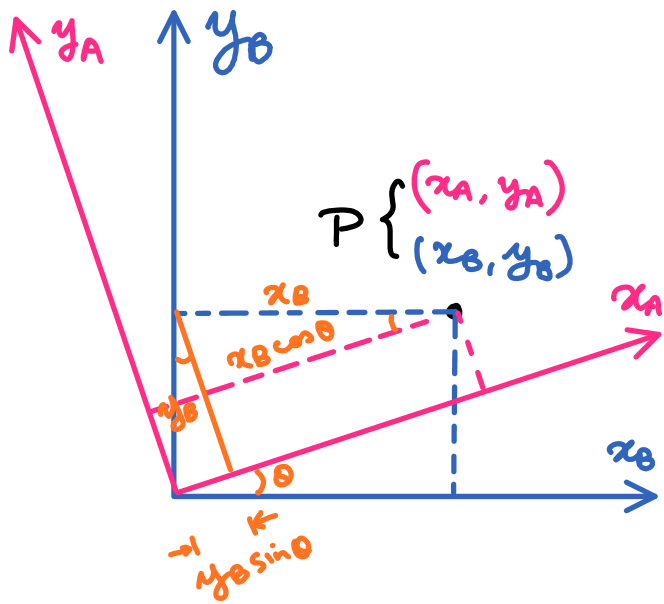
\includegraphics[width=\textwidth]{ss_trans}
	}
	I hope you get a better idea about the question by this analogue. Also, in the next section we will find a surprising similarity between these space-time and space-space transformations.
}

\mtextbox{Velocity in a general direction}{
	Be reminded that the relative velocity $v$ between frames is only along the $x$ direction (and positive for Bob). If you are dealing with velocities in a general direction $\mathbf{v} = (v_x, v_y, v_z)$, you can first do a rotation to rotate it to the $x$ direction before applying the transformation.
}
\textbox{Space transformation of a boost}{\index{Lorentz transformation: space}
	\twocol{0.55}{0.1}{0.35}{
		Given Bob's coordinate $(t_B, x_B)$, now we would like to solve $x_A$. How to do that? An equivalent question is that, how to physically describe $x_A$? Note that $x_A$ is Alice's spatial coordinate. Thus, if Alice carries a ruler (static wrt Alice) with length $x_A$, Alice holds one end, then the other end has coordinte $x_A$.
	}{
		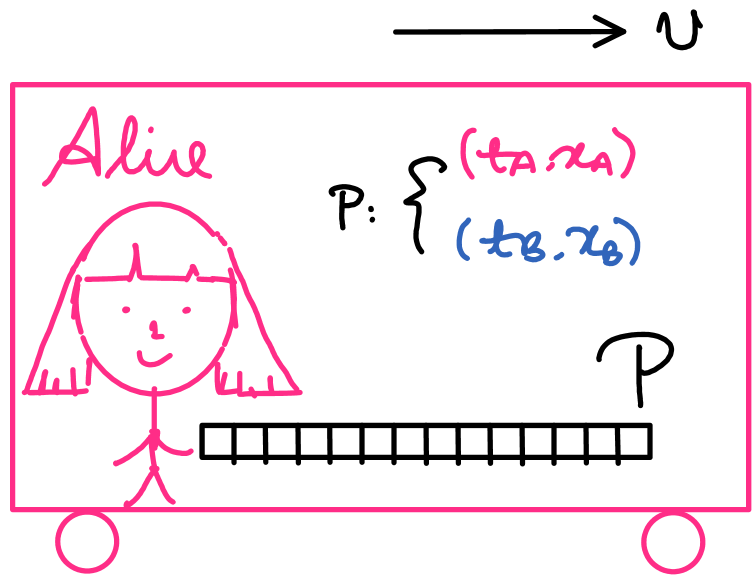
\includegraphics[width=\textwidth]{rr1_reduced}
	}

	\twocol{0.6}{0.05}{0.35}{
		For simplicity, we choose the same origin of coordinate for Bob and Alice. Given Bob's coordinate of P: $(t_B, x_B)$, how can we find the relation $x_A(t_B, x_B)$?
		
		Wrt Bob, the moving ruler has length $x_A/\gamma$. Thus at Bob's time $t_B=0$, the point P has $x_B=x_A / \gamma$. However, at $t_B\neq 0$, the end point P has also moved a distance $v t_B$. Thus for general $t_B$, $x_B = x_A/\gamma + v t_B$. In other words, we get $x_A(t_B, x_B)$ (i.e. $x_A$ as a function of $t_B$ and $x_B$) as
		\begin{align}
			\label{eq:st_space}
			x_A = \gamma \left ( x_B - v t_B \right )~.
		\end{align}
	}{
		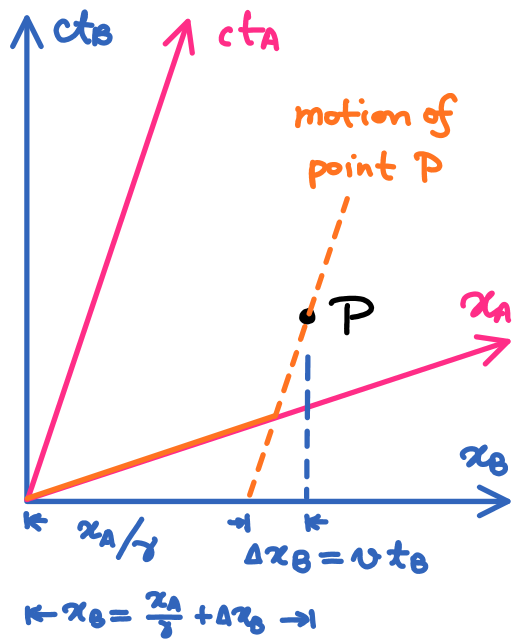
\includegraphics[width=\textwidth]{st_space_trans}
	}
	
	\tcblower

	How to get $t_B (t_A, x_A)$? We can flip Alice's and Bob's role and do the calculation again. But in fact we do not have to do it. Simply following $(\mathbb{R})$, we get
	\begin{align}
		\label{eq:st_space_r}
		x_B = \gamma \left ( x_A + v t_A \right )~.
	\end{align}
}

\mtextbox{Lorentz vs Einstein}{
	The Lorentz transformation is named after Lorentz for his work during 1892-1904. In other words, the Lorentz transformation is known before Einstein's special relativity (1905). It was discovered as mathematical symmetries behind the Maxwell equations and an phenomenological approach to explain the Michelson-Morley experiment. But it was Einstein who first understood the physics of such transformations.
}
\textbox{Time transformation of a boost}{\index{Lorentz transformation: time}
	The remaining question is: How to get $t_A(t_B, x_B)$ and $t_B(t_A, x_A)$? We do not have to do more thought experiments since we can solve them from equations \eqref{eq:st_space} and \eqref{eq:st_space_r}.

	Inserting \eqref{eq:st_space} into \eqref{eq:st_space_r} to eliminate $x_A$, 
	\begin{align}
	  \label{eq:stta}
	  x_B = \gamma \left [ \gamma \left ( x_B - v t_B \right ) + v t_A \right ]~.
	  \quad \rightarrow \quad
	  t_A = \gamma \left ( t_B - \frac{v}{c^2} x_B  \right )~.	  
	\end{align}
	Similarly, or simply using the principle of relativity, we get
	\begin{align}
	  \label{eq:stta_r}
	  t_B = \gamma \left ( t_A + \frac{v}{c^2} x_A  \right )~.  
	\end{align}
}

\mtextbox{The Lorentz symmetry}{
	Under the appearance of a transformation, a more physical name to refer to the equations \eqref{eq:ss-Lorentz} is the Lorentz symmetry: Alice and Bob are symmetric, in that though they use different coordinates to describe events, they observe the same laws of nature (for example, equations of motion for particles). Symmetry is now considered the first principle in fundamental physics. We will come back to the concept of symmetries in the part of action principle.
}
\textbox{Summary: the Lorentz transformation}{\index{Lorentz transformation}
	Let's summarize the transformation we have got, and add back the trivial $y$ and $z$ directions. These rules to transform between inertial frames is known as the Lorentz transformation. Here $\beta \equiv v/c$.
	\begin{equation}
		\label{eq:ss-Lorentz}
		\left\{
		\begin{aligned}
			c t_A & = \gamma ( c t_B - \beta x_B) \\
			x_A   & = \gamma ( x_B - \beta c t_B) \\
			y_A   & = y_B \\
			z_A   & = z_B
		\end{aligned}
		\right.
		\qquad\qquad\qquad
		\left\{
		\begin{aligned}
			c t_B & = \gamma ( c t_A + \beta x_A) \\
			x_B   & = \gamma ( x_A + \beta c t_A) \\
			y_B   & = y_A \\
			z_B   & = z_A
		\end{aligned}
		\right.
	\end{equation}
}

The Lorentz transformation describes the mathematical structure of special relativity. Thus our known results can be directly read-off from the formulas \eqref{eq:ss-Lorentz}.

\needspace{0.3\textheight}
\mtextbox{Why don't you tell us earlier?}{You may feel furious here: 
\mnewline
``I have spent great efforts in understanding time dilation, length contraction and simultaneity. But now they follow so simple equations. Why don't you start from telling us the Lorentz transformation and derive everything from there? That would have saved a lot of my time.''
\tcblower
I am in fact pretty careful in choosing the point to introduce Lorentz transformation. 
\mnewline
If I introduce it earlier, these effects will be just cold math formulas in your mind instead of living characters (i.e. with a physical picture). 
\mnewline
On the other hand, I can teach velocity addition, energy and momentum first and put the Lorentz transformation to the very end. But then the physical scenarios become too complicated to be helpful. I thus choose here to be the point to introduce this powerful tool.
}
\textbox{Time dilation, length contraction and simultaneity revisited}{
	\titem{
		\item Simultaneity: Consider two events $E_1$ and $E_2$, happened at the same time wrt Alice, i.e. $t^{E_1}_A=t^{E_2}_A$. Eq.~\eqref{eq:ss-Lorentz} gives $0=c(t^{E_1}_A-t^{E_2}_A) = \gamma [c (t^{E_1}_B-t^{E_2}_B)-\beta (x^{E_1}_B-x^{E_2}_B)]$. Clearly, if the two events happens at different locations and if $\beta\neq 0$, then the two events are not at the same time wrt Bob.

		\item Time dilation: A clock is moving wrt Alice with coordinate $(t_A, 0)$. Note that $x_A=0$ here since Alice carries the clock thus the clock is always located at the origin wrt Alice. From the first equation to the right panel of \eqref{eq:ss-Lorentz}, we get $t_B = \gamma t_A$.

		\item Length contraction: A ruler is moving together with Alice. How is Bob supposed to measure its length? Bob should measure his coordinates of both ends of the ruler \emph{at the same time}. The left end of the ruler is at $x_B=0$ when $t_B=0$. Thus the coordinate of the ruler at $t_B=0$ is the length of the ruler. From the second equation to the left panel of \eqref{eq:ss-Lorentz}, we get $x_B = x_A / \gamma$.
	}
}

Now we are ready to solve a problem: What's wrong with the Newtonian velocity addition rule $\mathbf{v}_B = \mathbf{v} + \mathbf{v}_A$ when $v_A\sim c$? In the optional material of the length contraction section, we studied a special case. Here we will derive general formulas.

\textbox{Addition of velocity}{\index{velocity addition}
	For simplicity, let us take the relative velocity $\mathbf{v}$ to be $(v, 0, 0)$, along the $x$-direction, as we have always assumed.

	Now Alice throw a ball with velocity
\begin{align}
  \label{eq:va}
  \mathbf{v}_A = (v_{Ax}, v_{Ay}, v_{Az}) 
  = \left( \frac{dx_A}{dt_A} , \frac{dy_A}{dt_A} , \frac{dz_A}{dt_A} \right)~.
\end{align}
and Bob finds
\begin{align}
  \mathbf{v}_B = (v_{Bx}, v_{By}, v_{Bz}) 
  = \left( \frac{dx_B}{dt_B} , \frac{dy_B}{dt_B} , \frac{dz_B}{dt_B} \right)~.
\end{align}
Now use the rule of Lorentz transformation, one can calculate
\begin{align}
  \label{eq:vbx}
  v_{Bx} = \frac{dx_B}{dt_B} 
  = \frac{\gamma d(x_A+v t_A)}{\gamma d\left(t_A + \frac{x_A v}{c^2} \right)}
  = \frac{dx_A+v dt_A}{dt_A + \frac{v}{c^2} dx_A} 
  = \frac{v_{Ax}+v}{1+\frac{v_{Ax}v}{c^2} }~.   
\end{align}
\begin{align}
  \label{eq:vby}
    v_{By} = \frac{dy_B}{dt_B} 
    = \frac{dy_A}{\gamma d \left ( t_A+\frac{v}{c^2} x_A \right )}
    = \frac{v_{Ay}}{\gamma \left(1+ \frac{v_{Ax} v}{c^2} \right)}~.  
\end{align}
Similarly,
\begin{align}
  \label{eq:vbz}
  v_{Bz} = \frac{v_{Az}}{\gamma \left(1+ \frac{v_{Ax} v}{c^2} \right)}~. 
\end{align}
}

\textbox{Example: velocity addition in perpendicular directions}{
	When $\mathbf{v}_A = (0, u, 0)$, perpendicular to the relative motion direction, we get
	\begin{align}
	  \label{eq:vex}
	  \mathbf{v}_B = \left ( v, u/\gamma, 0 \right )~.
	\end{align}
	Note that Alice and Bob measures different velocity even in the perpendicular direction, because their time intervals are different (while the length intervals are the same).
}

\section{The Geometry of Spacetime} \label{sec:geometry}

\textbox{Pythagoras theorem and modern geometry}{
	Since Gauss and Riemann, mathematicians realize that different types of geometry can be classified by how the Pythagoras theorem appears on those geometries. For example, on flat, spherical and hyperbolic surfaces, the Pythagoras theorem appears differently.
	\cg{0.7}{surf_geo}
	More careful studies on how the spherical and hyperbolic surfaces are curved, one can make the above expressions more precise and differentiate the relation twice to define spatial curvature.
	\tcblower
	Here we are not following this path to study pure spatial geometries in depth. Rather, we would like to ask the following question: Now that space and time are ``unified'' by Lorentz transformation, what does the spacetime geometry look like? Or what does the Pythagoras theorem look like for spacetime?
}

\marginnote{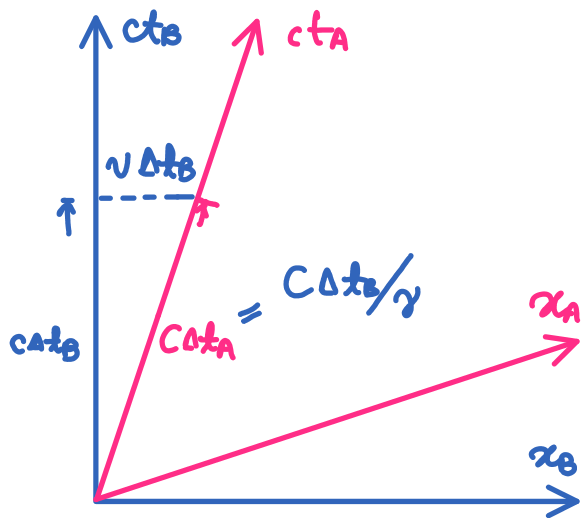
\includegraphics[width=0.3\textwidth]{st_geometry}}
\textbox{Our spacetime is NOT Euclidean}{
	Let us reconsider time dilation. Alice carries a clock and both Alice and Bob measure the tick-tock interval. 

	Wrt Bob, $\Delta t_B = \gamma \Delta t_A$. What does this imply on the spacetime diagram?

	Naively, from the geometry, we would have expected $c\Delta t_A > c\Delta t_B$, because $c\Delta t_A$ is the hypotenuse of the right triangle. However, from $\gamma>1$, we see  $c\Delta t_A < c\Delta t_B$. How is this possible?

	As we have discussed, we cannot take the Euclidean geometry for granted. 
	\marginnote{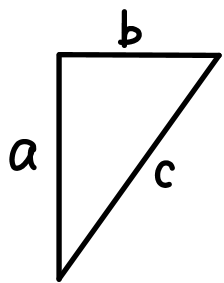
\includegraphics[width=0.1\textwidth]{st_right_tri}} 
	Especially, in the right figure, where $a$ and $c$ are time directions (of Alice or Bob), the Pythagorean theorem $a^2+b^2=c^2$ no longer holds. Instead, for time dilation,
	\begin{align}
	\label{eq:min_geo_tri}
	-a^2 + b^2 = -c^2 ~.
	\end{align}
	Extra minus sign emerges in front of the square of time, but not space. \marginnote{Note that minus sign in time squared indicates an extra factor of $i$ in front of time to match the Pythagoras theorem of flat space.} 

	Is it a coincidence, or is it in general a new type of geometry?
}

\mtextbox{Hyperbolic functions}{\index{hyperbolic functions}
	$\cosh x \equiv \frac{e^x+e^{-x}}{2}$ \mnewline
	$\sinh x \equiv \frac{e^x-e^{-x}}{2}$ \mnewline
	$\tanh x \equiv \sinh x / \cosh x$ \mnewline
	$\cosh^2 x - \sinh^2 x = 1$ \mnewline
	$\cosh(i\theta) = \cos\theta$ \mnewline
	$\sinh(i\theta) = i \sin\theta$
}
\textbox{Our spacetime is ALMOST Euclidean}{\index{Lorentz transformation and rotation}
	To see what has happened in another way, let us rewrite the Lorentz transformation using rapidity $\phi = \mathrm{arctanh}\beta$. Note that $\cosh \phi = \gamma$, and $\sinh \phi = \beta \gamma$. The Lorentz transformation is then
	\begin{equation}
		\left\{
		\begin{aligned}
			ct_B & =  ct_A \cosh\phi + x_A \sinh\phi \\
			x_B  & =  ct_A \sinh\phi + x_A \cosh\phi
		\end{aligned}
		\right.
	  \end{equation}
	Do you find it a bit similar to rotation?

	\tcblower

	Now let's apply a mathematical trick. Define
	\begin{align}
		\label{eq:theta}
		\phi \equiv i \theta ~, \qquad ct \equiv i w~.
	\end{align}
	We then get
	\marginnote{Do not ask me the ``physical meaning'' of the imaginarized time $w$ at the moment. Just consider it as a trick in math. In fact, there are profound implications of imaginary time in quantum field theory (zero temperature and finite temperature). But we are far not ready to introduce them here.}
	\begin{equation}
	\label{eq:ss-Lorentz-Euclidean}
	\left\{
	\begin{aligned}
		iw_B & = (iw_A)\cos\theta + x_A(i\sin\theta) \\
		x_B  & = (iw_A)(i\sin\theta) + x_A \cos\theta
	\end{aligned}
	\right.
	\quad\Rightarrow\quad
	\left\{
	\begin{aligned}
		w_B & = w_A\cos\theta + x_A\sin\theta \\
		x_B  & = -w_A\sin\theta + x_A \cos\theta
	\end{aligned}
	\right.
	\end{equation}
	This is \emph{exactly} a rotation of the $w$-$x$ plane, with $w$ considered as an extra spatial dimension!

	To summarize: A mathematical trick of redefining variables makes Lorentz transformation identical to rotation. 
}

\textbox{The symmetry of spacetime with imaginary time}{
	According to Pythagoras (570BC-495BC), sphere is the most beautiful and perfect object -- it is symmetric under 3 dimensional rotations.

	In this respect, our spacetime is even more beautiful than the most beautiful object. 
	\marginnote{We are not saying that spacetime is a sphere. Rather sphere is curved and our spacetime is flat in special relativity. However, its symmetry includes that of a sphere, and more (there are 4 additional spacetime translations).}
	This is because, now $w, x, y, z$ directions are no different from each other -- they are all related by rotation. Our spacetime is symmetric (i.e. laws of nature have the same form) under rotations in planes $w$-$x$, $w$-$y$, $w$-$z$, $x$-$y$, $x$-$z$, $y$-$z$, and all kinds of combinations of them. It is indeed more symmetric than a sphere because a sphere is only invariant under rotations in $x$-$y$, $x$-$z$, $y$-$z$ planes and their combinations.

	This further confirms that the difference between space and time is imaginary -- once you use imaginary time, time becomes no different from just another spatial direction, and the 3 boost along $x$, $y$ and $z$ directions just become three additional rotations.
}

\textbox{Natural units -- the units of nature}{
	In physics, some units are more natural than the others, because they use the same unit for the same things (or apparently different things, but with the same physical origin). 
	
	\marginnote{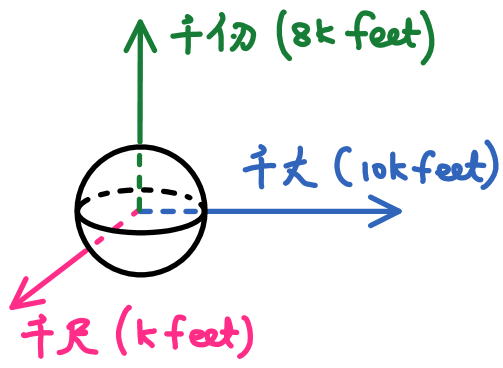
\includegraphics[width=0.3\textwidth]{natural_unit_rot}}
	Let's consider an example of a not-so-natural unit. In ancient China, sometimes people use a different unit for height of mountains. At that time, height seems different from other directions because of gravity. But now we see that the difference is due to the presence of the earth, which spontaneously break the symmetry of empty space. Fundamentally, height has no difference from the other two directions, and they can be related by rotation. Thus, we had better to use the same unit to measure height and the rest of the spatial dimensions.

	\mtextbox{Natural vs convenient}{
		The laws of nature are shorter in natural unit as unnecessary conversion of units are avoided. However, whether it is a convenient choice of unit depends on the physical context that we study. If we study explicit dynamics of systems with $v\ll c$, then we had better to keep $c$ explicit because otherwise we will deal with large/small numbers everywhere. For example, for $v=10^{-8}c \simeq 3$m/s, in natural unit the object only moves $10^{-8}$ unit of space in one unit of time.
	}

	\tcblower

	Now that we have seen space and time are not that different and can be related by Lorentz transformation, why we still give space and time different units? We don't have to.

	To use the same unit for space and time, we can just set $c=1$ and then speed is dimensionless. 

	This is known as the natural unit (together with $\hbar=k_B=1$). Natural unit is widely used in theoretical high energy physics.

	We shall not use natural units in this class and will always keep $c$ explicit.
}

\textbox{The invariant interval}{\index{invariant interval}\index{4-vector}\index{Minkowski space}

	In Euclidean space, 
	\begin{align}
	\label{eq:dse}
	ds^2 = dw^2 + dx^2 + dy^2 + dz^2~.
	\end{align}
	Recall that $w=-ict$. To bring us back to real time, we thus have
	\marginnote{In some books, the interval is defined as $ds^2 = d(ct)^2 - dx^2 - dy^2 - dz^2$. This is just a different convention without physical difference (corresponding to replacing all $ds^2$ here into $-ds^2$).}
	\begin{align}
	\label{eq:dsl}
	ds^2 = - d(ct)^2 + dx^2 + dy^2 + dz^2~.
	\end{align} 
	The importance of $ds^2$ is that, it is an invariant quantity under Lorentz transformation. To see that, one may first use $\{w, x, y, z\}$ and note that rotation keeps radius invariant. Or one can use the Lorentz transformation matrix to verify it explicitly. Just as $(\omega, x, y, z)$ forms a vector in 4d Euclidean space, $x^\mu = (ct, x, y, z)$ ($\mu=0,1,2,3$) also form a 4 dimensional vector (4-vector for short), which lives in the so called \emph{Minkowski space} -- which is just the mathematical name of our spacetime. \marginnote{In fact, our spacetime is more complicated than the Minkowski space -- in general relativity, you will see that our spacetime is curved instead of totally flat. This is considered to be more general spacetime but still with some Minkowski signature.}

	\tcblower 

	In fact, ``relativity'' is not a good name to the theory. By its name, it appears to emphasize that things are relative -- no longer as invariant as we thought. 
	
	But in fact, the essence of relativity is the other way round: Despite of being viewed from different perspectives (wrt different observers in different inertial frames), the events and their intrinsic relations are invariant.

	\marginnote{
		Recall the principles $(\mathbb{R})$, $(\mathbb{C})$ and $(\mathbb{E})$. Every each principle tell you a piece of invariance, instead of relativity.
		\mnewline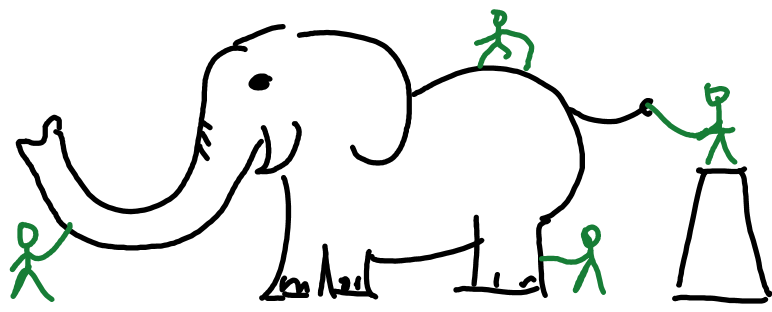
\includegraphics[width=0.42\textwidth]{touch_elephant}}
	Relativity is just the technology of study. But the spirit of the theory is the underlying invariance. 

	This is just like how you prove a theorem in Euclidean geometry -- it is not important if the figure is placed vertically or horizontally (i.e. wrt observers with different viewing angles). What's important is the intrinsic relation between the geometrical objects.  
	
	Another analogue is the story of blind men and an elephant. The goal of physics is to understand the elephant, instead of how different men feel differently by not being able to feel the whole thing.
}

\textbox{Time-like, space-like and null from the interval}{
	The sign of $ds^2$ corresponds to different types of separations of events:
	\begin{align}
		\label{eq:tsn}
		ds^2 < 0 &\quad\Leftrightarrow\quad \mbox{time-like} \nonumber\\
		ds^2 > 0 &\quad\Leftrightarrow\quad \mbox{space-like} \nonumber\\
		ds^2 = 0 &\quad\Leftrightarrow\quad \mbox{light-like, null}~.  
	\end{align}
	\tcblower
	And now you know why null is called null -- it is indeed null.  
}

\mtextbox{(Optional) Inner product of 4-vectors}{
	The invariant internal $ds^2$ can be considered as the inner product of 4-vector $dx^\mu$ with itself. In general, we can use the metric to measure the inner product to measure the inner product of any 4-vectors. For two 4-vectors $p^\mu$ and $k^\nu$, their inner product $\sum_{\mu\nu}g_{\mu\nu}p^\mu k^\nu$ is Lorentz invariant (i.e. invariant under Lorentz transformation).
}
\textbox{(Optional) A metric of spacetime}{\index{metric}
	A metric is a ``standard'' to measure coordinate distance. For our spacetime in special relativity, the metric $g_{\mu\nu}$ (as a symmetric $4\times 4$ matrix), infinitesimal coordinate distances and the invariant interval can be related as
	\begin{align}
		\label{eq:dsg}
		ds^2 = \sum_{\mu,\nu=0}^3 g_{\mu\nu} dx^\mu dx^\nu~,	  
	\end{align}
	where
	\begin{align}
	\label{eq:defg}
	x^\mu=\{ct, x, y, z\}~, \qquad g_{\mu\nu} = 
	\left( \begin{array}{cccc}
		-1 & 0 & 0 & 0 \\
		0 & 1 & 0 & 0 \\
		0 & 0 & 1 & 0 \\
		0 & 0 & 0 & 1
	\end{array} \right)~.
	\end{align}
	This seems to be a trivial rewriting of what we have obtained. However, here we have separated two different things:
	\begin{itemize}
		\item Coordinates $x^\mu$: What are the directions of spacetime?
		\item Geometry: What kind of geometry does spacetime satisfy?
	\end{itemize}

	Even if we use a different coordinate system, 
	\marginnote{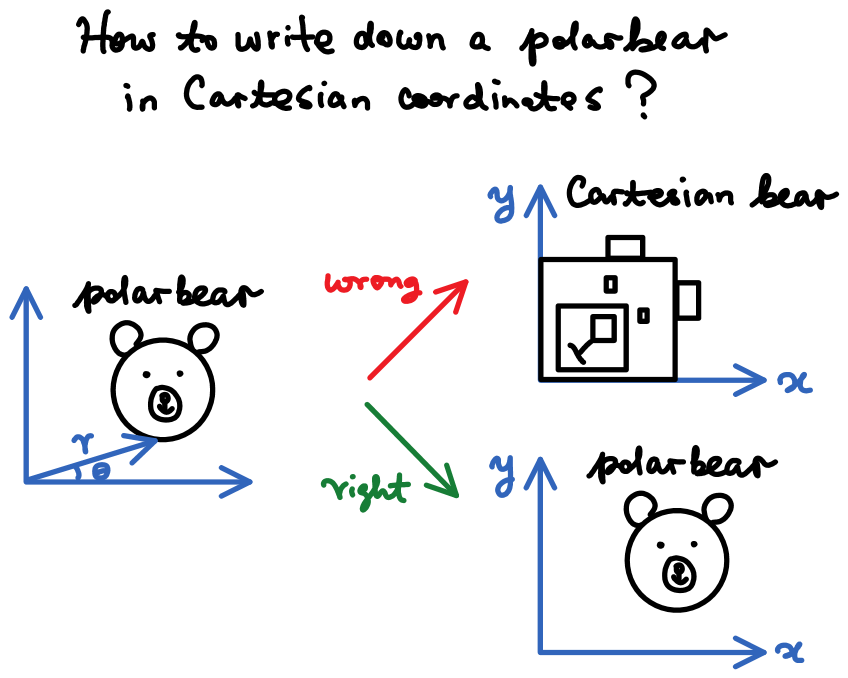
\includegraphics[width=0.3\textwidth]{polarbear}}
	for example, spherical coordinate for the spatial part, we can still choose a metric to keep $ds^2$ invariant:
	\begin{align}
		x^\mu=\{ct, r, \theta, \phi\}~, \qquad g_{\mu\nu} = 
		\left( \begin{array}{cccc}
			-1 & 0 & 0 & 0 \\
			0 & 1 & 0 & 0 \\
			0 & 0 & r^2 & 0 \\
			0 & 0 & 0 & r^2 \sin^2\theta
		\end{array} \right)~.
	\end{align}
	
	\tcblower

	In fact, the advantage brought about by a metric is not only the freedom to choose coordinates. Rather, it can describe the intrinsic curvature of spacetime which is not characterized by a different coordinate system. But this is beyond the scope of special relativity. You will see later that in general relativity, the metric $g_{\mu\nu}$ is the most important object to study. It can get curved by matter, and can guide matter how to move.
}

\section{Relativistic Momentum and Energy}\label{sec:momentum-energy}

Before
\mtextbox{Transforming Slimes}{
	Consider the following quiz: 
	\mnewline
	Suppose there are slimes of 3 shapes: $\triangle$, $\square$ and $\ocircle$. When slimes of differt shapes meet, they transform into the third shape. For example:
	$$
	\triangle + \square \rightarrow \ocircle \times 2 ~.
	$$
	Now that we have $\triangle\times 5$, $\square \times 7$ and $\ocircle \times 9$. Can you let them meet and transform them into $\triangle\times 6$, $\square \times 7$ and $\ocircle \times 9$ ?
	\mnewline
	Obviously not. Since the total number of slimes is conserved when they meet.
	\mnewline
	Fine. So, what about we have $\triangle\times 5$, $\square \times 7$ and $\ocircle \times 9$. Can you transform them into $\triangle\times 6$, $\square \times 9$ and $\ocircle \times 6$ ? 
	\mnewline
	Not either. Note that $(\#\triangle - \#\square) ~ \mathrm{mod} ~ 3$ is also conserved (where $\#$ denotes ``number of''). Which is violated.
	\tcblower
	Hope you get some feeling here that conserved quantities are helpful.
}
discussing energy and momentum in relativity, let us first recall why we need them at all. In Newtonian mechanics, it is nice to have energy and momentum because they are conserved. (See the below box for why conservation laws are good after all.) Thus in relativity, we should check if the Newtonian definition of energy and momentum are still conserved; and if not, how to generalize the definition of energy and momentum, to make them still conserved.

\textbox{What's good about conservation laws?}{\index{conservation laws: importance}
	\titem{
		\item Physically, conservation laws are the magic that we do not need to care what's happening in the middle. Given the initial state, we can immediately make a number of predictions (no greater than the number of conservation laws in the system).

		\item Mathematically, the equations of motion (like a set of $m \ddot x + V'=0$) are second order ordinary differential equations (ODEs) in $x$ which could be difficult. The conservation laws turns some of these into 1 or 0 order ODEs in $x$ which are much simpler (e.g. $\frac{1}{2} m\dot x^2 + V = E$, or charge conservation).

		\item Practically, in modern physics, the objects being studied are often extremely fast ($v\sim c$), small ($\Delta x\times \Delta p \sim \hbar$), heavy ($GM/(rc^2) \sim 1$), early (less than a second after the big bang), etc. It is often hard to directly build experiments to directly monitor exactly what is happening. Instead, one often needs conserved quantities to make useful observations. For examples, on modern colliders such as the Large Hadron Collider, the trajectories of particles (they are both small and fast in the above sense) are studied at a much later time compared to the time where interaction happened. If charge, energy or momentum were not conserved, it becomes much harder to study such particle physics processes (in fact, it will become not clear how to define observables even in principle without the help of energy and momentum conservation).
	}
	\tcblower
	That's cool. But why are we still lucky to have energy and momentum conservation in special relativity? In a later part ``From Action to Laws of Nature'', we will show you a positive answer -- the existence of these conservation laws are not a result of luck, but a result of the fact that no time moment or spatial location is special. This applies in special relativity as well as the Newtonian mechanics. Wait for that part if you are curious about the origin of these conservation laws.
}

\subsection{Relativistic Momentum}

\textbox{Can we still use Newtonian momentum conservation?}{\index{momentum: why not Newtonian}
	First, let us recall how the Newtonian momentum conservation are consistent with $(\mathbb{R})$ within Newtonian mechanics -- forget relativity for a moment here and assume $v\ll c$.

	For example, for Alice's momentum conservation for two particles:
	\begin{align}\label{eq:momentum_conservation}
		m_1 \mathbf{v}_1^A + m_2 \mathbf{v}_2^A = m_1 \mathbf{v}_1'{}^A + m_2 \mathbf{v}_2'{}^A~.
	\end{align}
	What will Bob find? In Newtonian mechanics, mass of the particles do not change. And velocity simply adds. Thus for Bob with a relative velocity $\mathbf{v}$, $\mathbf{v}_1^B = \mathbf{v}_1^A +\mathbf{v}$, etc. Thus, equation \eqref{eq:momentum_conservation} can be consistently written into the same form in Bob's frame:
	\begin{align}
		m_1 \mathbf{v}_1^B + m_2 \mathbf{v}_2^B = m_1 \mathbf{v}_1'{}^B + m_2 \mathbf{v}_2'{}^B~.
	\end{align}
	Happily, all the terms with $\mathbf{v}$ cancel in the above equation. So it takes the same form as \eqref{eq:momentum_conservation}. Thus, ($\mathbb{R}$) is indeed satisfied.
	  
	\tcblower

	Now, let us take relativity into account. For simplicity, let us assert that the mass of the particles still does not change with velocity. \emph{Assuming} that Alice still has the momentum conservation equation \eqref{eq:momentum_conservation}, then what will Bob find?

	\mtextbox{What if mass depends on velocity}{Indeed, we can assume that mass depends on velocity. We will get essentially the same relativistic momentum, just with a different definition of mass, the so called ``relativistic mass'': $m_{\mathrm{rel}} = \gamma m$. We will not use this notation.}

	Following the velocity addition rule, Bob finds (we only write the term for the first particle explicitly to emphasize the key points). Let the relative velocity between Alice and Bob be along the $x$ direction as usual. Then in the $x$ direction, we have:
	\begin{align}\label{eq:mom-wrong1}
		m_1 \frac{(v_{1Ax}+v)}{{\color{red}  (1 + \frac{v_{1Ax}v}{c^2} )}}  + \cdots
		=
		m_1 \frac{(v'_{1Ax}+v)}{{\color{red} (1 + \frac{v'_{1Ax}v}{c^2} )}} + \cdots ~.
	\end{align}
	In the $y$ direction (and $z$ direction has a similar equation), we have:
	\begin{align}\label{eq:mom-wrong2}
		m_1 \frac{v_{1Ay}}{{\color{red}\gamma (1+ \frac{v_{1Ax}v}{c^2} )}} + \cdots 
		= 
		m_1 \frac{v'_{1Ay}}{{\color{red}\gamma (1+ \frac{v'_{1Ax}v}{c^2} )}} + \cdots ~.
	\end{align}
	Unhappily, 
	\marginnote{The same argument applies to the Newtonian energy.}
	these equations \emph{do not} take the same form as \eqref{eq:momentum_conservation}, because of the red-colored factors. Thus, \eqref{eq:momentum_conservation} takes different form wrt Alice and Bob. It cannot be a piece of law of nature in special relativity.
}

\marginnote{In fact, we only need the energy and momentum \emph{differences} to return to Newtonian mechanics when $v\ll c$. You will find a surprise about energy in this respect soon.}
Now that we have seen the Newtonian energy and momentum are not conserved quantities (and the unexplained belief that there are still conserved energy and momentum after all), the best we can do is to search for new quantities in special relativity, where in the $v\ll c$ limit the quantity returns to energy and momentum in the Newtonian mechanics. 

\needspace{0.3\textwidth}
\mtextbox{Physical meaning of proper time}{
	Why a time variable can be defined \emph{independently of} an observer? Haven't we said that there is no absolute time? 
	\tcblower
	Because there exists a moving object (it moves, therefore it is). The moving object defines its own frame and thus defines its own time. In the own frame of the moving object, $d \mathbf{x}=0$. Thus indeed $d\tau = dt$. This verifies that the proper time is the time measured by the moving object itself. Imagine a clock moving together with the object. The proper time is the interval read from this clock.
}
\textbox{Using a proper time to fix momentum conservation}{\index{momentum}\index{proper time}
	How to fix the inconsistency of \eqref{eq:mom-wrong1} and \eqref{eq:mom-wrong2} with ($\mathbb{R}$)?

	If we can remove the red factor, we should be able to get a equation satisfying ($\mathbb{R}$). How? We recall that the red factor arises because
	\begin{align}
		dt_B = d \left[ \gamma \left( t_A + \frac{x_A v}{c^2} \right) \right] = \gamma (1+ \frac{v_{1Ax}v}{c^2} ) dt_A~.
	\end{align}
	
	In other words, every observer has their own time. Measuring motion with individual observer's own time ($d(\cdots) / dt_A$ and $d(\cdots)/dt_B$) is the root of evil.

	How can we get rid of the observer's own time in defining momentum? Or, is there an observer-independent way to measure a time-like interval?
	
	As I am trying to rephrase the question to approach the answer, now you should be able to figure it out: we have learned an observer-independent way to measure intervals using $ds^2$. To make a real number with correct time dimension, we define the \emph{proper time}:
	\begin{align}
		d\tau \equiv \sqrt{ - ds^2 /c^2} = \sqrt{dt^2 - \frac{dx^2}{c^2} } = \frac{dt}{\gamma}~. 
	\end{align}
	This is the time variable that we need. Thus, the momentum which gives a relativistic generalization of momentum conservation is
	\begin{align}
		\label{eq:ptau}
		\mathbf{p} = m \frac{d \mathbf{x}}{d\tau} 
		= \gamma m \mathbf{v}~. 	  
	\end{align}
	\tcblower
	From the first equal sign of equation \eqref{eq:ptau}, one observes that $\mathbf{p}$ transforms in the same way as $\mathbf{x}$ under Lorentz transformation. This is as promised that momentum conservation takes the same form in different frames. 
	
	However, this is confusing from another aspect: we know that space ($\mathbf{x}$) and time ($ct$) has combined into spacetime $(ct, \mathbf{x})$ in relativity as one entity. Now that momentum transform the same as space, is there a counterpart comes together which transform the same as time ($ct$)? What do we get if we naively replace $\mathbf{x}$ with $ct$ in \eqref{eq:ptau}? We get
	\begin{align}
		\label{eq:p0tau}
		\mbox{(the naive time-like counterpart of }\mathbf{p})
		= m \frac{d(ct)}{d\tau} = \gamma m c~. 
	\end{align}
	What's this? The nature should not leave it unexplained! We will return to this question in the next subsection.
}

Caution: Here we have only showed that the definition \eqref{eq:ptau} is consistent with $(\mathbb{R})$. We have not proved for you the actual conservation. In Newtonian mechanics, momentum conservation is derived from the 3rd law (which is an independent assumption from the Newtonian 1st and 2nd laws). Here we did not impose a 3rd law (although we can do so) and thus we do not have the right tool to derive momentum conservation. In fact, given an action, the relativistic momentum conservation can be derived from an action principle. We will not expand this point here.

\textbox{The relativistic force}{\index{force}
	Now that there is momentum, it is straightforward\marginnote{Here we use $dt$ instead of $d\tau$. This definition is convenient, because it is intuitive to think of force as one static observer pushes an object and see its acceleration -- how much additional efforts the static observer has to consume to push the rocket further.} to define force:
	\begin{align}
	\label{eq:force}
	\mathbf{F} \equiv \frac{d \mathbf{p}}{dt} = \frac{d (\gamma m \mathbf{v})}{dt} = \gamma m \dot{\mathbf{v}} + \gamma^3 m \mathbf{v} (\mathbf{v} \cdot \dot {\mathbf{v}}) / c^2~. 
	\end{align}

	Note that when $v\rightarrow c$, it takes $F\rightarrow \infty$ to change $v$. As a result, one can never accelerate a subluminal object to speed of light (or beyond). Thus $c$ is indeed the speed limit.
	\mtextbox{Chasing the light?}{When Einstein was 16 years old, he started to dream what would happen if he can run as fast as light. Would light stop oscillating and would that contradict Maxwell's theory of E\&M?
	\tcblower
	Now his dream has came to an end. No one can be accelerated to the speed of light and thus this seemingly contraditive thought experiment would never happen.}
}

\subsection{Relativistic Energy}

\textbox{The relativistic kinetic energy}{
	The relativistic force implies work to accelerate objects, and thus the kinetic energy. Consider an object initially at rest at location $x=0$, and is accelerated by a force in the $x$-direction, into a state with position $x$ and speed $v$. The work that the force has done turns into the kinetic energy of the object:
	\begin{align} \label{eq:ek}
		K = \int_0^x F ~ dx = \int_0^x \frac{d(\gamma m v)}{dt} ~ dx = \int_0^v v ~ d(\gamma m v) = (\gamma-1)mc^2~.
	\end{align}  
	In the second-to-last step we have converted the integration variable to $v$, and at the final step, we have performed integration by parts. The detail is left as an exercise.
	\tcblower
	A few comments in order before to proceed:
	\titem{
		\item When $v\ll c$ (so that we can do a Taylor expansion around $v\rightarrow 0$), the relativistic kinetic energy returns to our familiar Newtonian form as expected: $K\rightarrow \frac{1}{2} mv^2$.
		\item We have discussed kinetic energy following an acceleration process in the $x$-direction from rest. Is it general enough? Since kinetic energy is a label of a state, it should not care how it is obtained in the history of the object. Thus the kinetic energy is general enough no matter the force is not in the $x$-direction, or the object has an initial velocity.
	}


}

Now that we have the kinetic energy, what's the total energy? Before that, let us first study mass. In Newtonian mechanics (and chemistry), mass is conserved --  the total mass before and after a reaction is the same. What about in relativity?

\needspace{0.2\textheight}
\mtextbox{Does $v_y$ change?}{	
	No. Because we can view the event in another frame with $v_y=0$ at the beginning. Then in this frame $v_y=0$ at the end. Now switch to a frame with a small $v_y\ll c$. Using the velocity addition rule, $v_y$ does not change. (And the in $x$ direction $v_x$ only get a small correction of order $1/\sqrt{1-v_y^2/c^2}-1 = \mathcal{O}(v_y^2/c^2)$.)
}
\textbox{Mass is no longer conserved}{\index{mass: not conserved}
	We study a system split into two objects. Consider two objects connected by a spring. The spring is compressed and stores some potential energy. Initially the objects are at rest. The initial mass of the whole system is $M$. After releasing the spring, the two objects move apart, each has mass $m$ and moving apart with speed $v$.

	\cg{0.5}{e-split} 
	
	In Newtonian mechanics, 
	there is no doubt that $M=2m$. But is it true when $v\sim c$?

	\tcblower

	To study the property of the system, 
	we add a small probe velocity in the $y$ direction $v_y \ll v$ (One can comfortably take $v_y$ to be infinitesimal). Then interestingly, momentum conservation in the $y$ direction can calculate $M$ for us.

	\titem{
		\item Before the split: $p_y = M v_y$.
		\item After the split: $p_y = 2\gamma m v_y$ for the same $p_y$ (momentum conservation), where $\gamma = 1/\sqrt{1-v^2/c^2}$ accounts not only velocity in the $y$ direction, but the the total velocity.
	}

	Thus, $M=2\gamma m > 2m$! The good old mass conservation breaks down.
}

\textbox{The relativistic rest energy}{
	Consider the above $M\rightarrow 2m$ split process. Let's consider the limit $\gamma \gg 1$, i.e. the final objects are flying very close to the speed of light. In this limit, the kinetic energy of the final objects are $K\simeq 2\gamma m c^2$. 
	\marginnote{The two final objects also has their rest energies, $mc^2$ each. In our $\gamma\gg 1$ limit, these rest energies can be neglected. In fact, initially Einstein used light to derive the relativistic energy, corresponding to no rest mass. But the derivation needs more understanding of E\&M than assumed in this course. We thus follow another route here.}
	
	From energy conservation, the kinetic energy of the final objects is contained in the initial object. Thus, the energy of the initial object is
	\begin{align} 
		E = 2\gamma m c^2 = M c^2. 
	\end{align}
	Recall that the initial object is at rest. Thus, the energy here is the rest energy of an object.
	\tcblower
	\index{rest energy}
	\mtextbox{Daily energy usage of Hong Kong}{To see the huge rest energy of matter, for example, the daily energy consumption of Hong Kong is of order $10^{15}$J. That corresponds to about $10$ grams of matter -- about the weight of one AAA battery. To compare, the chemical energy that an AAA battery can provide is a few thousand joules.}
	The rest energy
	\begin{align} \label{eq:e0}
		E_\mathrm{rest} = mc^2	
	\end{align}
	is the part of energy that an object has, even if it is not moving at all. This energy is huge in our daily standard since $c$ is a huge number in our daily life (and we have $c\times c$). 
	
	In Newtonian mechanics, due to mass conservation, this energy is not noticed in energy conservation. However, in relativistic situations this energy can be released. For example,

	\mtextbox{Why do stars shine?}{Before relativity was understood, there was a big mystery that how stars can shine for longer than the human history, if the stars are powered by chemical energy. Instead, the nuclear fusion in the star can power the stars for billions of years.}
	\titem{
		\item We have already encountered a non-trivial case of rest energy above -- the two final objects after the split having $E=M c^2 > 2mc^2$. 
		\item In more realistic situations, the usage of nuclear energy makes use of the rest energy of matter. In nuclear fissions and fusions, a much greater amount of energy can be released compared to usual chemical or mechanical reactions. 
		\item In labs, one can collide particles and anti-particles. The particles disappear after they meet and the rest energy can be completely released in the form of light. 
		 
	}	
}

\mtextbox{The zero-point of rest energy}{The particle-anti-particle annihilation phenomenon is a very important check about the concept of rest energy. Because the zero point of energy makes no physical sense unless all the energy can be released.}
\textbox{The relativistic energy}{\index{energy}
	In general, for an object with mass $m$ and speed $v$, combining the kinetic energy \eqref{eq:ek} and the rest energy \eqref{eq:e0}, the total energy of the object is
	\begin{align} \label{eq:relei}
		E = \gamma m c^2 ~.
	\end{align}
	\tcblower
	This sounds a bit different from what you heard: $E=mc^2$. This more famous formula (famous because without having to explain $\gamma$ in popular science) may stand for one of the two meanings:
	\titem{
		\item The rest energy of an object.
		\item The total energy of an object, with the mass defined as the velocity-dependent ``relativistic mass'' $m_\mathrm{rel} \equiv \gamma m$ and thus $E=m_\mathrm{rel} c^2$. Nowadays we understand mass as a Lorentz invariant label of a particle; the convention of $m_\mathrm{rel}$ is seldomly used and thus we will not use $m_\mathrm{rel}$ further here.
	}
}

\needspace{0.2\textheight}
\mtextbox{Light is light}{
	Applying \eqref{eq:mep} to light, we have $v=c$. Thus, $m=0$. In other words, if we view light as particles (see the quantum mechanics part for more information), their mass has to vanish.
	\tcblower
	The 4-vector of the momentum of light has the form $p^\mu = (E/c, \mathbf{p})$, where the energy of light $E = c |\mathbf{p}|$. This 4-vector has vanishing Lorentz norm. In the notation of the metric (optional material), we have $\sum_{\mu, \nu} g_{\mu\nu}p^\mu p^\nu=0$.
}
\textbox{The 4-dimensional momentum vector}{\index{4-momentum}\index{invariant mass}
	Remember the question we asked at \eqref{eq:p0tau}? Happily, up to a factor of $c$ (which is nothing more than a conversion of unit as we have explained natural unit), the energy we have got in \eqref{eq:relei} is exactly the missing ``naive time-like counterpart of momentum'' in \eqref{eq:p0tau}. The 4 dimensional momentum is then $p^\mu = (E/c, \mathbf{p}) = (\gamma mc, \gamma m\mathbf{v}) = \gamma m \dot x^\mu$.

	Recall that for the spacetime coordinate 4-vector, we have an invariant quantity $c^2 \Delta t^2 - \Delta x^2$. Is there a counterpart for the momentum 4-vector? Yes. Squaring equation~\eqref{eq:relei}, we get
	\begin{align}\label{eq:mep}
		m^2 c^4 = E^2 - \frac{v^2}{c^2} E^2	= 
		\xlongequal{\mbox{using ratio of \eqref{eq:relei} and \eqref{eq:ptau}}}
		E^2 - p^2 c^2~.
	\end{align}
	Thus, though $E$ and $\mathbf{p}$ are dependent on observers, the combination on the RHS is independent of observers, but is just the invariant mass squared of the particle. This is not surprising. Because the momentum and coordinate 4-vectors lives in the same space and is measured by the same metric. (Just as it is not surprising that both the magnitude of 3d coordinate vector and 3d momentum are rotational invariant.)
}

\textbox{(Optional) The relativistic Doppler effect of light}{
	Alice is moving with 3-velocity $\mathbf{v}$ wrt Bob. If Bob observes that the energy of light is $E_B$, what's the corresponding energy $E_A$ of the same beam of light in Alice's frame?

	We can solve this problem by the Lorentz invariance of inner products of 4-vectors. The inner product $\sum_{\mu\nu}g_{\mu\nu}k^\mu p^\nu$ is invariant under Lorentz transformations, where $k^\mu$ and $p^\nu$ are the 4-vector of Alice's momentum and the momentum of the beam of light.

	In Bob's frame: $k^\mu = (\gamma m c, \gamma m \mathbf{v})$, $p^\nu = (E_B/c, \mathbf{p})$. The Lorentz invariant inner product is $\sum_{\mu\nu}g_{\mu\nu}k^\mu p^\nu = -\gamma m (E_B-\mathbf{v}\cdot\mathbf{p})=-\gamma m E_B (1 - (v/c) \cos\theta)$, where $\theta$ is the angle between $\mathbf{v}$ and $\mathbf{p}$ in Bob's frame.

	In Alice's frame: $k^\mu = (mc, \mathbf{0})$, $p^\nu = (E_A/c, \mathbf{p'})$. The Lorentz invariant inner product is $\sum_{\mu\nu}g_{\mu\nu}k^\mu p^\nu = - m E_A$. It must be equal to the Lorentz invariant in Bob's frame. Thus, $E_A = \gamma E_B (1 - (v/c) \cos\theta)$. 
	\tcblower
	From 
	\marginnote{Here the purpose of this optional box is not only to tell you the formula of the relativistic Doppler effect, but also to show the power of Lorentz invariance for the inner product. The Doppler effect can also be derived just by considering the effect of time dilation and space contraction. But the calculation is much more complicated for a general direction $\theta$.}
	either classical E\&M or quantum mechanics, we will find that the frequency of light is $\omega \propto E$. Thus the frequency of light wrt Alice and Bob has a similar relation $\omega_A = \gamma \omega_B (1 - (u/c) \cos\theta)$.
}

\section{Epilogue: Summary and What's Next}

The below diagram is a recap of what we have learned. The green color denote external contents (you may ignore) and the blue denote alternative logic.

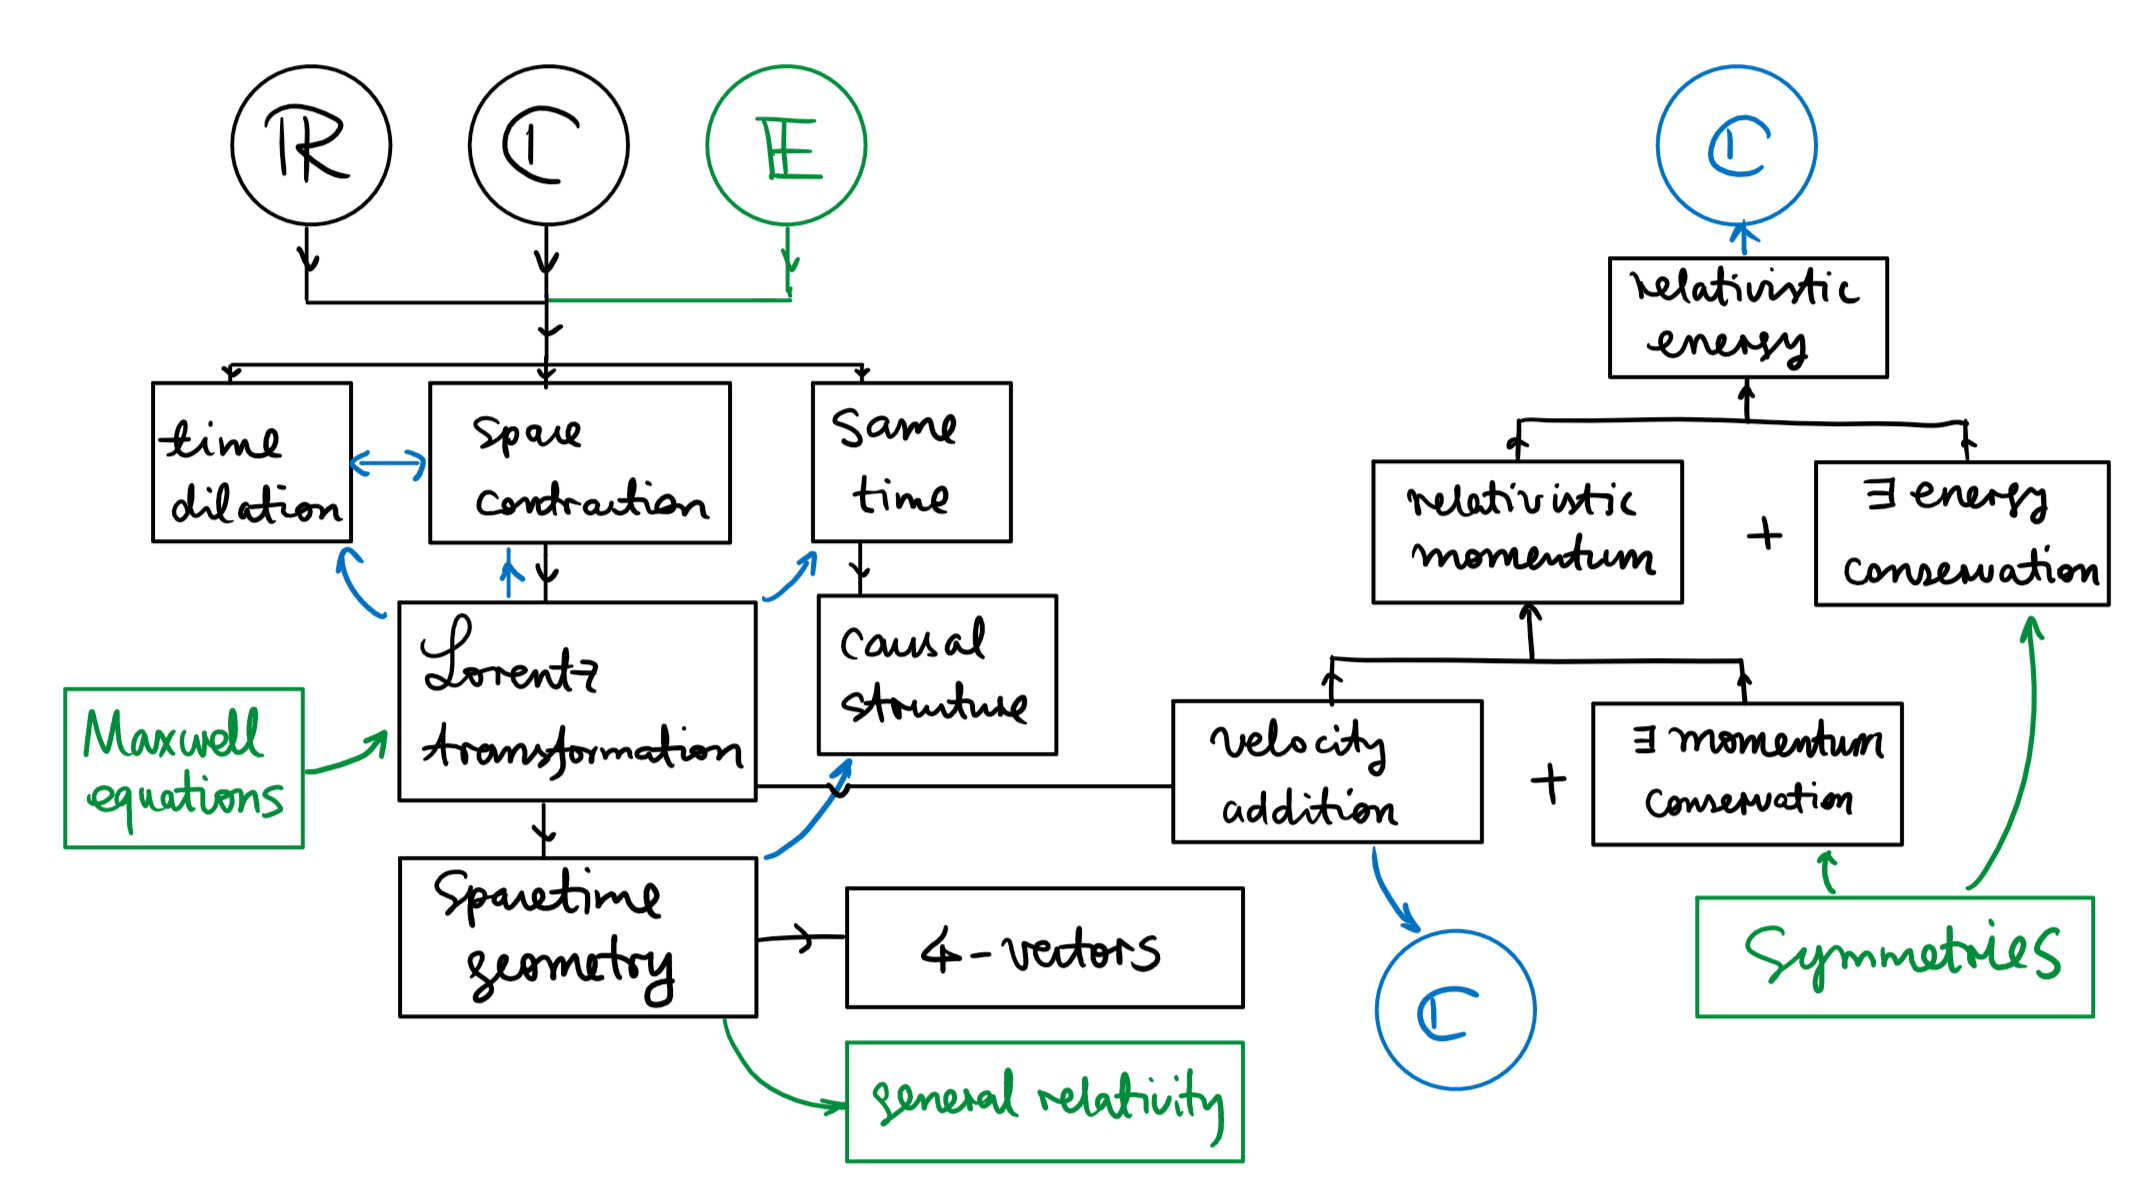
\includegraphics[width=1.3\textwidth]{summary_relativity}

\textbox{Further reading about the content}{
	\titem{
		\item If you are interested to explore more about the geometry of spacetime and formulate special relativity with geometrical emphasize, read \href{https://www.amazon.com/Spacetime-Physics-Edwin-F-Taylor/dp/0716723271}{``Spacetime Physics''} by Taylor and Wheeler (and the a few general relativity books below).
		\item If you are not happy about our guess of relativistic energy and momentum, but rather want to derive them, wait and we will do it in the part ``From Action to Laws of Nature''. See also \href{
			http://theoreticalminimum.com/}{``Theoretical Minimum'' (Video Lectures)} by Susskind.
		\item If you consider the math used this text too sloppy, read \href{https://www.amazon.com/Relativity-Special-Cosmological-Wolfgang-Rindler/dp/0198567324}{``Relativity: Special, General, and Cosmological''} by Rindler.
		\item If you like to learn more about the relation between electrodynamics and relativity before getting to the full details of electrodynamics, read \href{
			http://www.damtp.cam.ac.uk/user/db275/concepts/Concepts.pdf}{Lecture Notes on Modern Physics} by Baumann.
		\item Many good books on general relativity also starts with a dense and high-level introduction of special relativity, for example \href{https://www.amazon.com/Gravity-Introduction-Einsteins-General-Relativity/dp/0805386629}{Gravity: An Introduction to Einstein's General Relativity} by Hartle, \href{https://www.amazon.com/Gravitation-Charles-Misner/dp/0691177791}{Gravitation} by Misner, Thorne and Wheeler and \href{https://www.amazon.com/Gravitation-Cosmology-Principles-Applications-Relativity/dp/8126517557}{Gravitation And Cosmology} by Weinberg.
	}
}

\textbox{What happens next in a university physics program?}{
	\titem{
		\item Electrodynamics as a deeper study of E\&M.
		
		When Einstein was young, he was deeply puzzled by two observations. Both has roots in E\&M. One is light cheasing, which you have understood by now. The other was the magnet-conductor paradox, as he emphasized in the first paragraph of his 1905 paper. The paradox is shown in the below figure:

		\cg{1}{magnet-conductor-paradox}
		
		Before special relativity, the Coulomb law and the Lorentz law are considered as two independent fundamental laws of nature. However, by a change of frame, in the moving-magnet frame, the induct current is explained using the Coulomb law and in the moving-conductor frame the induced current is explained using the Lorentz law. This indicates that one should not consider them both fundamental -- one same thing shouldn't be explained by two fundamental principles in physics! If the Coulomb law is more fundamental (at least it is more familiar), we should be able to derive the Lorentz law from it.

		How relativity helps? Roughly speaking, 3-dimensional vectors such as $\mathbf{E}$ and $\mathbf{B}$ should be extended into 4-dimension vectors. Thus, the Coulomb and Lorentz laws, depending only on $\mathbf{E}$ and $\mathbf{B}$, respectively, should be combined into one law using the form of 4-velocity and 4-electric-magnetic vector.

		Without getting into the math, let us use a thought experiment to intuitively understand how to ``derive'' Lorentz force from Coulomb force by a change of frame. 

		Consider a wire conducing electric current, and a charge. The wire and the charge has relative motion between each other. 
		
		\cg{1}{e_and_m}

		Here the Lorentz force is derived by the different amount of length contraction effect of moving charges. 
		
		In electrodynamics, you will explore the full connection between E\&M and relativity.

		\item You may learn how special relativity works with gravity in ``general relativity''. We will also have a part to mention it briefly.
		\item Symmetry, transformation and group. Einstein's postulates (to be more precise, the Lorentz transformation) has the mathematical structures of a group (Lorentz group). ``Group theory'' is widely used in physics, including relativity, particle physics and solid state physics. And they are of their own importance in math as well. 
		\item You may learn how special relativity works with quantum mechanics in ``quantum field theory''. 
	}
}

\section{Exercises}

% Sec 1

\textbox{E\wref{sec:principles-relativity}.1 Plain waves}{
	Consider ``plain wave'' $e^{ik(x-ct)}$. Interpret the real part of $e^{ik(x-ct)}$ as the amplitude of the wave. 
	\tenum{
		\item For fixed $t$, show the plain wave indeed looks like a wave.
		\item Figure out the moving direction and speed of the wave.
	}
}

% Sec 2

\needspace{0.2\textwidth}
\marginnote{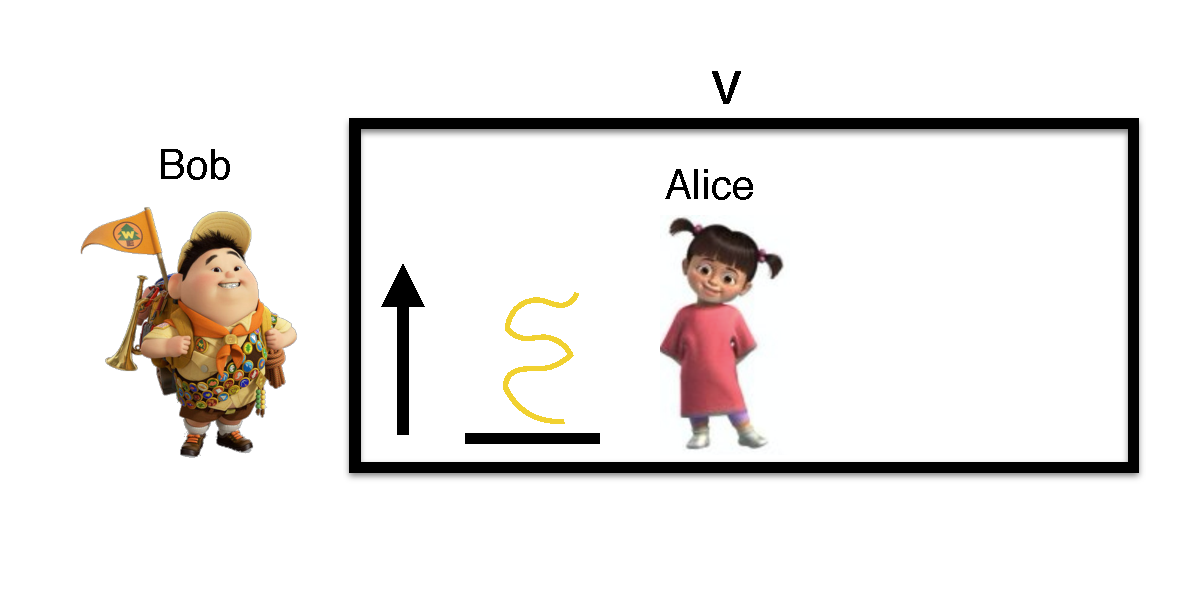
\includegraphics[width=0.25\textwidth, trim={0 0 200pt 0}, clip]{E1.pdf}}
\textbox{E\wref{sec:time-dilation}.1 Light travel and time dilation}{
	Consider Alice and Bob have relative motion against each other, with velocity $v$. Alice carries a candle, which emits light (speed of light is $c$) perpendicular to the motion direction (wrt Alice). 
	\tenum{
		\item What's the speed of this light ray wrt Bob? 
		\item What's the travel direction of this light ray wrt Bob? 
		\item Wrt Bob, the time of Alice slows down. Why doesn't the speed of this light ray slow down? Explain the relation between slower time and speed of light.
	}
}

% Sec 5

\marginnote{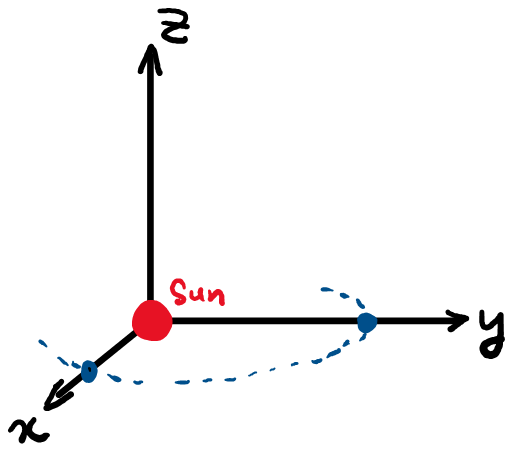
\includegraphics[width=0.25\textwidth, trim={0 2pt 2pt 0}, clip]{earth-sun}} 
\textbox{E\wref{sec:same-time}.1 Spacetime diagram of the sun-earth system}{
	Use the frame that the sun is static, draw a spacetime diagram of the sun's and the earth's motion in $x$-direction (a direction in the earth's orbit plane). Show on this diagram how the sunlight (emitted in the $x$-direction) reaches the earth. The vertical axis is $ct$.
}

\textbox{E\wref{sec:same-time}.2 Spacetime diagram with constant proper acceleration}{
	Alice is moving with constant ``proper acceleration'' in the $x$-direction: $x^2 - t^2=$constant (to simplify the discussion, let's work in one spatial dimension only). Not all light towards the observer can reach Alice. The region where light cannot reach Alice is called the ``Rindler horizon''. Draw a spacetime diagram of Alice's motion and find where the Rindler horizon is.
}

\textbox{E\wref{sec:same-time}.3 What the twin actually sees}{
	Draw the spacetime diagram of the twin paradox and show what the static twin actually sees (i.e. in the order that light reaches his eyes) about the aging of the moving twin (when she was moving outwards and when she was moving back).
}

\textbox{E\wref{sec:same-time}.4 Distance between spaceships.}{
	An observer A is considered at rest in the whole setup of this question. Two spaceships B and C are equidistant to A and are initially also at rest, and the distance between them is $L$. Now A sends a light signal. After receiving the light signal, B and C immediately start to move at a velocity $v$ in the same direction (neglect the period of acceleration). What is the distance between B and C after they are moving? Give your answer wrt A and wrt B, respectively. Hint: draw a spacetime diagram to find out what happened.
}

% Sec 6

\textbox{E\wref{sec:lorentz}.1 Use Lorentz transformation in calculations}{
	Use Lorentz transformation to calculate:
	\tenum{
		\item Time dilation.
		\item Rule contraction.
		\item For two events which happened at the same time wrt Alice, calculate the time difference wrt Bob, given Bob's speed $v$, and the distance between the two events being $L$ wrt Alice. % Lv/c^2
	}
}

\textbox{E\wref{sec:lorentz}.2 Examples of velocity addition}{
	Alice is moving away from Bob with velocity $\vec v =(v,0,0)$, and sending out light rays.
	\tenum{
		\item If the light ray is along $x_A$ direction ($x$ direction wrt Alice), calculate the velocity of the light ray $\vec v_B = (v_{Bx},v_{By},v_{Bz}) $ wrt Bob.
		\item If the light ray is along $y_A$ direction ($y$ direction wrt Alice), calculate the velocity of the light ray $\vec v_B = (v_{Bx},v_{By},v_{Bz}) $ wrt Bob.
	}
}

\textbox{E\wref{sec:lorentz}.3 Speed of light in the media}{
	Consider the speed of light in static air (refractive index $n=1.0003$). How does the speed of light in the air change wrt moving observers moving with speed $v$? How does the speed of light in the air change when there is a wind with speed $v$?
}

% Sec 7

\textbox{E\wref{sec:geometry}.1 The spacetime interval is Lorentz invariant}{
	Show that under Lorentz transformation, the spacetime interval $ds^2$ is unchanged (although $t$ and $x$ change). For simplicity, work in two dimensions $t$ and $x$ only (i.e. no motion or rotation in $y$ and $z$ directions).
}

\textbox{E\wref{sec:geometry}.2 Our motion in spacetime}{
	Show that using proper time, everyone is moving in spacetime (not space) with the same 4-speed (i.e. the size of the 4-velocity $dx^\mu / d\tau$).
}

\textbox{E\wref{sec:momentum-energy}.1 Integrate momentum to get energy}{
	Let us use the relativistic momentum $p=\gamma mv$ to derive the expression of the kinetic energy, in a different way from what we did in class. 

	Consider a ball at rest at $x=0$ with mass m, and act a constant force $F$ on this ball toward the $x$ direction. The ball then accelerates because of the force.

	Note that $F=dp/dt$, and the kinetic energy can be calculated from the work done by the force: 
	\begin{align}
	K= \int_0^{x_1}F~dx= \int_0^{x_1} \left(\frac{dp}{dt}\right)dx=\int_0^{p_1}v~dp=\int_0^{v_1}v~d(\gamma mv)~,
	\end{align}
	where $x_1$, $p_1$ and $v_1$ are the distance, momentum and velocity at a later time $t_1$.

	Continue the calculation and derive the kinetic energy of the ball at time $t_1$.	
}

\textbox{Read Einstein's original papers on relativity}{
	Nowadays Einstein's original papers can be easily found online. For example, \href{https://www.fourmilab.ch/etexts/einstein/specrel/www/}{his first paper}. You will find most parts the paper accessible except that in electrodynamics he used different notations from modern convention. 
}

\printindex

\end{document}
